\documentclass[
12pt, % The default document font size, options: 10pt, 11pt, 12pt
%oneside, % Two side (alternating margins) for binding by default, uncomment to switch to one side
english, % ngerman for German
doublespacing, % Single line spacing (singlespacing), alternatives: onehalfspacing or doublespacing
%draft, % Uncomment to enable draft mode (no pictures, no links, overfull hboxes indicated)
%nolistspacing, % If the document is onehalfspacing or doublespacing, uncomment this to set spacing in lists to single
liststotoc, % Uncomment to add the list of figures/tables/etc to the table of contents
%toctotoc, % Uncomment to add the main table of contents to the table of contents
%parskip, % Uncomment to add space between paragraphs
%nohyperref, % Uncomment to not load the hyperref package
headsepline, % Uncomment to get a line under the header
chapterinoneline, % Uncomment to place the chapter title next to the number on one line
%consistentlayout, % Uncomment to change the layout of the declaration, abstract and acknowledgements pages to match the default layout
openany, % eliminates all extra blank pages from entire document
]{DoctoralThesis}



\usepackage[table]{xcolor}

\usepackage{array} 
\usepackage{comment}
\usepackage{graphicx}
\usepackage[T1]{fontenc}
\usepackage{csquotes}
\usepackage{balance}
\usepackage{setspace}

\usepackage{lstautogobble}
\usepackage{subcaption}

\usepackage{standalone}
\usepackage{algorithmicx}

\usepackage{amsmath}
\usepackage{amssymb}

\usepackage{tikz}
\usepackage{soul}
\newcounter{row}
\newcounter{col}
\newcommand\setrow[6]{
  \setcounter{col}{1}
  \foreach{} \n in {#1, #2, #3, #4, #5, #6} {
    \edef\x{\value{col}-0.5}
    \edef\y{6.5-\value{row}}
    \node[anchor=center] at (\x, \y) {\n};
    \stepcounter{col}
  }
  \stepcounter{row}
}

\newcommand{\chapterabstract}[1]{
    \begin{quote}
        \singlespacing\small
        \rule{13cm}{1pt}

        #1
        \vskip-4mm
        \rule{13cm}{1pt}
\end{quote}}

\usepackage{lineno}
\linenumbers{}

\usepackage[normalem]{ulem}

\usepackage{hyperref}
\hypersetup{hidelinks}

\usepackage{listings}
\lstset{ %
language=C++,                % choose the language of the code
basicstyle=\ttfamily\footnotesize,       % the size of the fonts that are used for the code
commentstyle = \color{ForestGreen},
columns=fullflexible,
numbers=left,                   % where to put the line-numbers
numberstyle=\footnotesize,      % the size of the fonts that are used for the line-numbers
stepnumber=1,                   % the step between two line-numbers. If it is 1 each line will be numbered
numbersep=5pt,                  % how far the line-numbers are from the code
%backgroundcolor=\color{codeBG3},  % choose the background color. You must add \usepackage{color}
showspaces=false,               % show spaces adding particular underscores
showstringspaces=false,         % underline spaces within strings
showtabs=false,                 % show tabs within strings adding particular underscores
frame=single,           % adds a frame around the code
tabsize=2,          % sets default tabsize to 2 spaces
captionpos=b           % sets the caption-position to bottom
breaklines=true,        % sets automatic line breaking
breakatwhitespace=false,    % sets if automatic breaks should only happen at whitespace
keywordstyle=\color{blue},       % keyword style
  %language=Octave,                 % the language of the code
  otherkeywords={SearchVar,MV,TSS,tileExpr,Search},           % if you want to add more keywords to the set
  numberstyle=\tiny\color{black}, % the style that is used for the line-numbers
  rulecolor=\color{black},
escapeinside={<@}{@>}
} 
\definecolor{ForestGreen}{RGB}{34,139,34}
\newcommand{\todo}[1]{{\textcolor{red}{{\tt{TODO:}}\,\,#1 }}}
\newcommand{\nc}[0]{\todo{cite}}
\newcommand{\an}[1]{{\textcolor{blue}{Author's Note: #1}}}
\newcommand{\ttt}[1]{{\texttt{#1}}}
\usepackage{xspace}
\newcommand{\FormatDecisions}[0]{{\textsc{FormatDecisions}}}
\newcommand{\su}[1]{{#1$\times$}}
\graphicspath{{./graphics/}{.}{./graphics/FormatDecisions}{./graphics/RAJALC}{../sparseEval}{./graphics/SparseRAJA}}

\usepackage[subtle]{savetrees}
\vbadness=18000


\newcommand{\dense}[0]{{\textsc{dense}}}
\newcommand{\specialized}[0]{{\textsc{specialized}}}
\newcommand{\sparseraja}[0]{{\textsc{sparseraja}}}
\newcommand{\SpMV}[0]{{SpMV}}
\newcommand{\GauSei}[0]{{GauSei}}
\newcommand{\InCholFact}[0]{{InCholFact}}

\usepackage{makecell}

\thesistitle{Type the title of your thesis here} % Your thesis title, this is used in the title, committee approval and abstract pages, print it elsewhere with \ttitle

\chair{Michelle Mills Strout} % Your dissertation chair's name, this is used in the title, abstract and committee approval pages, print it elsewhere with \chairname

\cochair{David Lowenthal} % Your dissertation co-chair's name, this is not currently used anywhere in the template, but would be used in the title and committee approval page, print it elsewhere with \cochairname

\examiner{Type the name of your examiner here} % Your examiner's name, this is not currently used anywhere in the template, print it elsewhere with \examname

\degree{Type the name of your degree here} % Your degree name, this is used in the title page and abstract, print it elsewhere with \degreename

\author{Brandon Neth} % Your name, this is used in the title page and abstract, print it elsewhere with \authorname

\addresses{Type your address here} % Your address, this is not currently used anywhere in the template, print it elsewhere with \addressname

\subject{Type your subject area here} % Your subject area, this is not currently used anywhere in the template, print it elsewhere with \subjectname

\keywords{Type keywords here} % Keywords for your thesis, this is not currently used anywhere in the template. However, you may want to use it following your abstract, print it elsewhere with \keywordnames

\university{University of Arizona} % Your university's name and URL, this is used in the title page and abstract, print it elsewhere with \univname

\department{Department of Computer Science} % Your department's name and URL, this is used in the title page and abstract, print it elsewhere with \deptname

\facultyA{Type the name of your committee member here} % Your first faculty member's name and URL(can be added between green curly brackets before the member's name. Do not use this for your COMMITTEE CHAIR This is used in the committee approval page, print it elsewhere with \facnameA

\facultyB{Type the name of your committee member here} % Your first faculty member's name and URL(can be added between green curly brackets before the member's name. This is used in the committee approval page, print it elsewhere with \facnameB

\facultyC{Type the name of your committee member here} % Your first faculty member's name and URL(can be added between green curly brackets before the member's name. This may optionally be added to the committee approval page when number of committee members requires it, print it elsewhere with \facnameC

\facultyD{Type the name of your committee member here} % Your first faculty member's name and URL(can be added between green curly brackets before the member's name. This may optionally be added to the committee approval page when number of committee members requires it, print it elsewhere with \facnameD

\defense{Type defense date here} % This should have the long date format of your scheduled defense, print it elsewhere with \defensedate

\AtBeginDocument{
\hypersetup{pdftitle=\ttitle} % Set the PDF's title to your title
\hypersetup{pdfauthor=\authorname} % Set the PDF's author to your name
\hypersetup{pdfkeywords=\keywordnames} % Set the PDF's keywords to your keywords
\hypersetup{hidelinks} % Set all hyperlinks standard color text
}


\begin{document}

%
%\frontmatter % Uncomment to use roman page numbering style (i, ii, iii, iv...) for the pre-content pages

\pagestyle{plain} % Default to the plain heading style until the thesis style is called for the body content


%-------------------------------------------------------------------------------------------------------------------------------
%	Pre-Thesis Content
%-------------------------------------------------------------------------------------------------------------------------------

%----------------------------------------------------------------------------------------
%	TITLE PAGE
%----------------------------------------------------------------------------------------
%
% All requirements of the graduate college as of 2019-01-30
% The title page must be the first page of your document (All pages must be numbered and match 
% the numbers listed in Table of Contents. However, a page number is not required to be printed
% on the actual title page).
% The title page must meet the following requirements:
% Title is set in ALL CAPS
% Student name matches official name in UAccess
% Rule line appears
% Official Department Name is Used
% Degree is indicated correctly
% Copyright year matches year of graduation on page

\begin{titlepage}
\begin{singlespacing} % needed for documents set to 1.5 or 2.0 spacing, Comment out otherwise
\begin{center}

\vfill

\MakeUppercase{\ttitle}\\ %Thesis Title in ALL CAPS
\vspace{0.4in}
by\\ \vspace{0.4in}
{\authorname}\\ % Places author name as specified in preamble
\vspace{0.6in}
\HRule \\[0.1cm] % Horizontal line
Copyright \textcopyright\space\authorname\space{\the\year}\\ % Copyright Date

\vspace{0.4in}

A Dissertation Submitted to the Faculty of the\\ % University required text
\vspace{0.4in}
\MakeUppercase{\deptname} \\  % Department name in Small Caps
\vspace{0.4in}
In Partial Fulfillment of the Requirements \\ \medskip % University required text
For the Degree of \\  % University required text
\vspace{0.4in}
\MakeUppercase{\degreename} \\ % Thesis type
\vspace{0.4in} 
In the Graduate College \\  % University required text
\vspace{0.4in}
\MakeUppercase{The \univname} \\ % University name in Small Caps
\vspace{0.6in}
%\normalsize
{\the\year}\\[4cm] % date
%\includegraphics{Logo} % University/department logo - uncomment to place it

\vfill
\end{center}
\end{singlespacing}% needed for documents set to 1.5 or 2.0 spacing, Comment out otherwise
\end{titlepage}

%\cleardoublepage %Uncomment to add blank page after Title page.


\setcounter{page}{2} % Starts pagination at 2 on the Committee Approval Form with no page number displayed on Title page.

%----------------------------------------------------------------------------------------
%	COMMITTEE APPROVAL PAGE
%----------------------------------------------------------------------------------------
%
% All requirements of the graduate college as of 2019-01-30
% The committee approval page must be the second page of your document
% The committee approval page must meet the following requirements:
% Title on approval page matches title on page 1 (Title Page)
% Dissertation chair (or co-chair) is indicated
% All members and chair (or co-chairs) have signed the approval page
% Date of defense is listed

%\addchaptertocentry{Committee Approval Page} % Add the committee approval page to the table of contents
\begin{singlespacing} % needed for documents set to 1.5 or 2.0 spacing, Comment out otherwise
\begin{center}
%\large

THE \MakeUppercase{\univname} \\
GRADUATE COLLEGE
\end{center}

\vspace*{0.3in}

\noindent As members of the Dissertation Committee, we certify that we have read the dissertation prepared by \authorname \space entitled "\ttitle "\space and recommend that it be accepted as fulfilling the dissertation requirement for the Degree of \degreename.

\vspace*{0.3in}

\noindent\underline{\makebox[4.0in][r]{}} \hspace{0.4in} Date: \defensedate \\
{\bfseries\chairname}\\
\emph{(Chair)} %This line can be commented out if necessary
\vspace*{0.3in}

\noindent\underline{\makebox[4.0in][r]{}} \hspace{0.4in} Date: \defensedate \\
{\bfseries\facnameA}\\
\emph{(Member)} %This line can be commented out if necessary
\vspace*{0.3in}

\noindent\underline{\makebox[4.0in][r]{}} \hspace{0.4in} Date: \defensedate \\
{\bfseries\facnameB}\\
\emph{(Member)} %This line can be commented out if necessary
\vspace*{0.3in}

\noindent\underline{\makebox[4.0in][r]{}} \hspace{0.4in} Date: \defensedate \\
{\bfseries\facnameC}\\
\emph{(Member)} %This line can be commented out if necessary
\vspace*{0.5in}

% If 4th committee member is needed, copy the preceding 4 lines, change to facnameD in copied lines
% You will then need to adjust vertical spacing to keep committee approval page to 1 page length

\noindent Final approval and acceptance of this dissertation is contingent upon the candidate's submission of the final copies of the dissertation to the Graduate College.

\vspace*{0.2in}

\noindent I hereby certify that I have read this dissertation prepared under my direction and recommend that it be accepted as fulfilling the dissertation requirement.
\vspace*{0.5in}

\noindent\underline{\makebox[4.0in][r]{}} \hspace{0.4in} Date: \defensedate \\
Dissertation Director: \chairname \\
%{\bfseries \emph{Instructor \\ Hispanic Linguistics}} % Update hard-coded to job title and department
\vfill
\end{singlespacing}% needed for documents set to 1.5 or 2.0 spacing, Comment out otherwise



%----------------------------------------------------------------------------------------
%	STATEMENT BY AUTHOR
%----------------------------------------------------------------------------------------
%
% No longer required for the graduate college as of 2019-01-30
% Uncomment all lines in this section  with "%%" at the beginning if your document requires it

%%\begin{statement}
%%\begin{singlespacing} % needed for documents set to 1.5 or 2.0 spacing, Comment out otherwise
%%\addchaptertocentry{\authorshipname} % Add the declaration to the table of contents

%The following block of text was the required text of the Graduate College (2019-02-01)
%%This dissertation has been submitted in partial fulfillment of the requirements for an advanced degree at the \univname\space and is deposited in the University Library to be made available to borrowers under rules of the Library. \\ \smallskip 

%%Brief quotations from this dissertation are allowable without special permission, provided that an accurate acknowledgement of the source is made. Requests for permission for extended quotation from or reproduction of this manuscript in whole or in part may be granted by the copyright holder.

%%\vspace*{0.3in}
%%\begin{center} 
%%SIGNED: \authorname
%%\end{center}
%%\end{singlespacing}% needed for documents set to 1.5 or 2.0 spacing, Comment out otherwise
%%\end{statement}


%----------------------------------------------------------------------------------------
%	ACKNOWLEDGEMENTS
%----------------------------------------------------------------------------------------
%
% Acknowledgements are not a necessary item. Comment out if not being used 
%\include{FrontBackMatter/Acknowledgements} % This calls the Acknowledgements.tex 


%----------------------------------------------------------------------------------------
%	DEDICATION
%----------------------------------------------------------------------------------------
%
% Dedications are not a necessary item. Comment out to remove from document
\dedicatory{For my \ldots \\\bigskip Dedicated to my \ldots.} 


%----------------------------------------------------------------------------------------
%	Quotation
%----------------------------------------------------------------------------------------
%
% This page is not really necessary, but if you feel the need to include some quote here is your
% chance. 
%
% Comment out if not being used 
%\include{FrontBackMatter/Quotation} % This calls the Quotation.tex


%----------------------------------------------------------------------------------------
%	LIST OF CONTENTS/FIGURES/TABLES PAGES
%----------------------------------------------------------------------------------------
%
% Table of Contents (TOC) must include:
% a: all major sections with the document in a consistent manner
% b: section headings in document must match their listings (exact words) in TOC
%
\tableofcontents % Prints the main table of contents
%
% Lists of figures and tables must include accurate page numbers
\listoffigures % Prints the list of figures

\listoftables % Prints the list of tables


%----------------------------------------------------------------------------------------
%	ABBREVIATIONS
%----------------------------------------------------------------------------------------
%
% Abbreviations are not a necessary item. Comment out the line below to remove from document
%
%


%----------------------------------------------------------------------------------------
%	PHYSICAL CONSTANTS/OTHER DEFINITIONS
%----------------------------------------------------------------------------------------
%
% Constants are not a necessary item. Comment out the line below to remove from document
%
%\include{FrontBackMatter/Constants} % This calls the Constants.tex Uncomment to include


%----------------------------------------------------------------------------------------
%	SYMBOLS
%----------------------------------------------------------------------------------------
%
% Symbols are not a necessary item. 
%
% Comment out if not being used 
%
%\include{FrontBackMatter/Symbols} % This calls the Symbols.tex Uncomment to include


%----------------------------------------------------------------------------------------
%	Abstract
%----------------------------------------------------------------------------------------
% This is required to appear before the first chapter of the dissertation

%\include{FrontBackMatter/Abstract} % This calls the Abstract.tex


%\chapter{Introduction}

High performance computer simulation plays a foundational role in modern science and engineering.
For example, considering the nine-figure cost of a utility-scale wind farm~\cite{wiser2022land}, there is significant interest in ensuring the farm will behave as expected. 
Computer simulation can help provide this confidence.

When developing these types of applications, three competing concerns need balanced. 
First is developer productivity.
From the earliest days of electronic computing~\cite{backus1957fortran} to today, code has been expensive to write.
High-productivity languages like Python excel in the realm of developer productivity.
While the actual execution of the code is slow, the ease of writing, maintaining, and updating the code can make up for the slow performance.
However, in many situations, such as HPC, the code also needs to run quickly.
The second competing concern is exactly this: application performance.
There are often real-world constraints on how long code execution can take.
Consider the automatic braking system in many modern vehicles.
These systems do not have the luxury of running slowly, else they risk the safety of their passengers.
On the other end, large simulation codes need to make the most out of the limited time they are allotted on HPC systems.
Writing fast code runs at odds with programmer productivity in part because achieving good application performance normally requires the use of languages like C++ and Fortran, languages rarely lauded for developer productivity.
The final competing concern, cross-system portability, runs in tension with both application performance and programmer productivity.
Computing hardware is diversifying, meaning code optimized for one system may perform poorly on another.
Finding one set of optimizations that give good performance across different systems is not straightforward, and not even always possible.
The alternative is to maintain multiple versions of the same code base, each specially optimized for the system it is designed for.

In developing HPC applications, DoE places emphasis on creating codes that run performantly on many different systems.
Performance portability libraries like RAJA~\cite{hornung2014RAJA}, Kokkos~\cite{edwards2014kokkos}, and YAKL~\cite{norman2022portable} address this problem by surfacing the performance ``knobs'' that an engineer can use to tune an application for a particular system. 
These include loop schedule transformations --- like loop interchange, tiling, vectorization, OpenMP threading, offloading to accelerators --- and global data format transformations.
While powerful, this approach focuses on tuning each loop independently, leaving out opportunities for optimizations that are applied across loops.
A programmer who wishes to apply valuable cross-loop optimizations like loop fusion~\cite{mckinley1996improving}, overlapped tiling~\cite{bertolacci2019using,zhou2012hierarchical,CathieSC14}, or inter-loop layout changes~\cite{kennedy1995automatic,kennedy1998automatic} cannot do so without breaking the abstractions of the performance portability library.
This sacrifice of portability for performance is also present for a programmer who wishes to express parts of a computation that work with sparse data.
This dissertation seeks to remedy this problem, introducing abstractions to support cross-loop schedule and data transformations and laying the foundation for native support for sparse computations within the RAJA library.

\section{Programming with Performance Portability Libraries}
Performance portabile libraries are driven by the need to create modularized and easily-tuned code.
This is achieved through a process of decomposing the computation into seperable parts.
While the specifics of this decomposition differ across libraries, they share key components.
Broadly, these components appear as data abstractions and operation/execution abstractions.
Here, I demonstrate these abstractions using a 5-point stencil computation, broken into Listings~\ref{stencilData},~\ref{stencilKernel}, and~\ref{stencilSchedule}.
This computation uses two $N \times M$ arrays \verb.A. and \verb.B..


\subsubsection{Data Abstractions}
\begin{figure}
\begin{lstlisting}[caption={Data declaration using RAJA multi-dimensional data abstractions, called Views. Changing a View's layout only requires changing the second argument in its constructor.}, label=stencilData]
using namespace RAJA;

//Create an array with the dimension extents...
std::array<size_t, 2> dimLengths = {N,M};

//Create the layout type...
auto rowMajor = make_layout(dimLengths, {0,1}); //dim0, then dim1
auto colMajor = make_layout(dimLengths, {1,0}); //dim1, then dim0

//Then initialize the Views...

//with row-major storage
View<double,2> A(new double[N*M], rowMajor);
View<double,2> B(new double[N*M], rowMajor);

//OR

//with column-major storage
View<double,2> A(new double[N*M], colMajor);
View<double,2> B(new double[N*M], colMajor);
\end{lstlisting}
\end{figure}

Multi-dimensional data is exceedingly common in simulation codes.
However, a computer's memory is addressable only as a one-dimensional sequence of bytes.
Thus, any multi-dimensional representation must be mapped to the 1-dimesional nature of the hardware.
Usually, this is achieved by breaking the data into one-dimensional strips and storing each strip in sequence.
Different ways to break the data into strips produce different orders of elements within memory.
Two of these layouts that are well-known are the two dimensional column-major and row-major storage formats.
Here, the strips of two-dimensional data are either the columns or the rows.

Called a View in RAJA and Kokkos and an Array in YAKL, multidimensional data structures are a key abstraction through which these embedded libraries surface portability controls to the programmer.
When tuning an application for a new system, changing the layout of data in memory can have large performance implications.
These differences are especially relevant between different processor types, where a data layout that performs well on a CPU is not best for a GPU\@.
It can also impact performance between two CPUs because of threading and cache behaviors~\cite{trott2021kokkos}.


Traditional approaches to representing multi-dimensional data, such as the array of pointers or vector of vectors, do not admit an easy data layout change.
This is due to the high degree of coupling between the layout and the method of data access. 
For example, using these approaches, an access to the $(i,j)$th entry of a two dimensional structure will look like this: \verb.A[i][j]..
Should the programmer want to try a column-major ordering instead of the default row-major, their only option is to completely transpose the data structure.
This process starts with the cumbersome but managable task of redeclaring the sizes of each dimension in the structure's initializiation, switching the dimensions' extents.
Then, every single access to the structure needs to be changed. 
All instances \verb.A[i][j]. must become \verb.A[j][i]..
This is a enormous task, and one where well-camouflaged bugs are born. 
In a paragraph of prose, \verb.[i][j]. is easily distinguished from \verb.[j][i]..
In a complicated loop nest making hundreds of data accesses, all using different orderings of the iterators, one forgotten (or extra) swap quickly creates crashes.
And of course, once the transformation has been applied and the new bugs squashed, it may turn out that a layout change had no effect, or even a negative one.

The multi-dimensional abstractions in P3 libraries bring the cost of such a transformation back to the scale of the programmer's thought-loop by introducing layout polymorphism.
In Kokkos and YAKL, this polymorphism is restricted to compile-time.
In RAJA, this polymorphism is restricted to runtime at the point of initialization.
Regardless of where and how the programmer selects the layout specifically, the key idea here is that changing one thing about a data structure only requires changing one thing in the code.
Listing~\ref{stencilData} shows the process of initializing two Views and highlights the minimal code changes required to switch between different layouts.

\subsubsection{Operation/Execution Abstractions}
\begin{figure}
\begin{lstlisting}[caption={Specification of a 5-point stencil kernel using RAJA.}, label=stencilKernel]
//Declare a lambda that executes one iteration of the computation...
auto stencilLambda = [=](int i, int j) {
  B(i,j) = 0.2 * (A(i,j) + A(i-1,j) + A(i+1, j) + A(i,j-1) + A(i,j+1));
};

//Create the iteration space...
auto iDimension = RangeSegment(1,N-1);
auto jDimension = RangeSegment(1,M-1);
auto iterationSpace = make_tuple(iDimension,jDimension);

//Define the kernel execution policy...
using SequentialPolicy = KernelPolicy<
  statement::For<0,seq_exec, //Sequential outer loop traverses iDimension
    statement::For<1,seq_exec, //Sequential inner loop traverses jDimension
      statement::Lambda<0> //Calls lambda
    >
  >
>;

//Launch!
kernel<SequentialPolicy>(iterationSpace, stencilLambda);
\end{lstlisting}
\end{figure}

As with their data abstractions, P3 libraries share an approach to their abstractions for specifying and executing the operations of a computation.
At a high level, the computation is decomposed into an operation describing what to do, an iteration space describing which values to do it for, and scheduling information describing how to order and distribute them among the different processing elements.
This process is shown for a 5-point stencil computation in Listing~\ref{stencilKernel}.

All three libraries share their use of functors to represent the operation of an individual iteration.
Often represented using a lambda closure, these loop body statements form the basis for the description of a computation.
Parameters to the lambdas represent the indices of an iteration space point. 
An example of such a lambda is shown on lines 1--4 of Listing~\ref{stencilKernel}.

The iteration space is specified as a tuple of containers.
In Listing~\ref{stencilKernel}, lines 6--9 show this process for the 5-point stencil. 
The \verb.RangeSegment. function creates a range from its first argument to its second.

Last is the schedule for the computation.
In RAJA, this comes in the form of the kernel policy.
Lines 11--18 of Listing~\ref{stencilKernel} show the policy that describes the canonical sequential schedule.
Changing parts of the kernel policy change the execution schedule. 
Listing~\ref{stencilSchedule} shows some of these changes: one for loop interchange, one for OpenMP parallelization and vectorization, and one for loop tiling.

Once these components are specified, they are combined and executed using the \verb.kernel. method, shown on the final line of Listing~\ref{stencilKernel}.
Changing the loop schedule of the computation is as simple as changing the template argument to the call to a different policy.


\begin{figure}
\begin{lstlisting}[caption={Kernel policies for different loop schedules.}, label={stencilSchedule}]
using OpenMPwithVectorization = KernelPolicy<
  statement::For<0,omp_parallel_for_exec, //Parallel outer loop traverses iDimension
    statement::For<1,simd_exec, //Vectorized inner loop traverses jDimension
      statement::Lambda<0>
    >
  >
>;

using Interchanged = KernelPolicy<
  statement::For<1,seq_exec, //Sequential outer loop traverses jDimension
    statement::For<0,seq_exec, //Sequential inner loop traverses iDimension
      statement::Lambda<0>
    >
  >
>;

using ParallelTiled = KernelPolicy<
  statement::Tile<0, tile_fixed<64>, omp_parallel_for_exec, //Parallel tiling loop
    statement::Tile<1, tile_fixed<64>, seq_exec, //Sequential tiling loop
      statement::For<0,seq_exec, //Within tile, iDimension
        statement::For<1,simd_exec, //Within tile, jDimension
          statement::Lambda<0>
        >
      >
    >
  >
>;
\end{lstlisting}
\end{figure}

\section{Optimization Scope}

The transformations that these libraries surface to the programmer support a common paradigm for program optimization: profile, identify an expensive loop or kernel, try a transformation, and repeat.
Using this paradigm, each kernel is optimized as a standalone piece of code.
While useful for leveraging the maximum possible parallelism from an application, it draws attention away from the interrelation of the kernels.
This means that important opportunities for performance optimization can go overlooked.

\subsection{Inter-Loop Transformations}
Transformations at the inter-loop scope often target the reuse of data between loops.
In computations bottlenecked by data transfer speeds, like sparse computations and the stencil computation above, these optimizations are especially beneficial. 
Two examples are overlapped tiling and inter-kernel layout transformations.

\subsubsection{Loop Fusion}
\begin{figure}
\begin{lstlisting}[caption={Three loops, with and without loop fusion.},label=fusionExample]
//without fusion
for(int i = 0; i < N; i++) {
  A1(i) = A0(i) * 2;
}
for(int i = 0; i < N; i++) {
  A2(i) = A1(i) - 1;
}
for(int i = 1; i < N-1; i++) {
  A3(i) = A2(i-1) / 2;
}

//with fusion
//iterations outside of the shared iteration space
A1(0) = A0(0) * 2;
A1(N-1) = A0(N-1) * 2;
A2(0) = A1(0) - 1;
A2(N-1) = A1(N-1) - 1;

//fused component
for(int i = 1; i < N-1; i++) {
  A1(i) = A0(i) * 2;
  A2(i) = A1(i) - 1;
  A3(i) = A2(i-1) / 2;
}
\end{lstlisting}
\end{figure}

Loop fusion is a well-known optimization for improving data locality, appearing as an automated transformation in source to source compilers in the mid 90s~\cite{mckinley1996improving}, but was in use decades before~\cite{warren1984hierarchical,cocke1971catalogue}.
A simple example of this transformation is shown in Listing~\ref{fusionExample}.
Rather than computing and storing the entirity of the intermediary arrays, loop fusion allows for the values to be used as soon as they are produced, when the value may still even be in the CPU's registers.
However, loop fusion can interfere with the parallelization of the loops being fused.
Newer transformations, like overlapped tiling, have been developed to achieve the locality improvements of loop fusion while maintaining sufficient parallelism.

Overlapped tiling~\cite{holewinski2012high,krishnamoorthy2007effective} maintains parallelism by introduces small amounts of recomputation.
In this transformation, each tile overlaps with those next to it, sharing some points of the iteration space.
By choosing tile sizes that keep the fraction of recomputation low, parallel execution of the tiles still benefits from improved locality.
This transformation has been ncorporated into an OpenCL compiler by Zhou et al~\cite{zhou2012hierarchical} and Polymage~\cite{mullapudi2015polymage}, a DSL for image processing pipelines, incorporates overlapped tiling into its automatic optimization passes.
These approaches do not allow for programmer control over the tiling process.
Halide~\cite{ragan-kelley2013halide}, another DSL for image processing pipelines, surfaces control over tiling to the programmer.
For the optimization of existing codes, Bertolacci et al~\cite{bertolacci2019using} develop an approach based on pragma directives.

\subsubsection{Layout Changes}
\begin{figure}
\begin{lstlisting}[caption={Changing a View's data layout between computations by hand.},label={FormatChangeByHand}]
//C = A * B
auto knl1 = make_kernel<KPOL>(segs1, [=](auto i0, auto i1, auto i2) {
	C(i0, i1) += A(i0, i2) * B(i2, i1);
});

//E = A^T * D
auto knl2 = make_kernel<KPOL>(segs2, [=](auto i0, auto i1, auto i2) {
	E(i0, i1) += A(i2, i0) * D(i2, i1);
});

knl1();

// Reorder A's data for column-major order
double * tmp1 = new double[n*n];
for(int i = 0; i < n; i++) {
	for(int j = 0; j < n; j++){
		tmp1[j*n + i] = A(i,j);
	}
}
memcpy(A.data, tmp1, n*n);
A.layout = colMajor;
delete[] tmp1;

knl2();
\end{lstlisting}
\end{figure}

If two computations access the same data in different orders, it can be worthwhile to change how that data is organized in memory so that both computations access the data in the most efficient way possible.
As a simple example, consider the matrix multiplication $C = A * B$ followed by the matrix multiplication $E = A^{\top} * D$. 
The way these computations will traverse the matrix $A$ is different. 
In the computation of $C$, the data of $A$ is traversed across the rows, while in the computation of $E$, it is traversed across the columns.
Assume for a moment that $A$ is stored in row-major order.
Because the $C$ computation traverses the data of $A$ by rows, adjacent iterations will access elements of $A$ that are adjacent in memory.
This has much more favorable cache behavior than the computation of $E$, where adjacent iterations access elements of $A$ that are more distant in memory.
Performance can be improved by changing the layout of $A$ between the two computations, ensuring that both kernels have favorable access patterns.
However, applying such a transformation by hand is, as discussed above, time consuming and error prone. 
An example of such a manual implementation of this transformation is shown in Listing~\ref{FormatChangeByHand}.

Early work on the problem of automatically selecting data layouts were done in the High Performance Fortran and D programming languages using graph theoretic formulations, specifically for distributed computing systems\cite{kennedy1995automatic,kennedy1998automatic}.
Later work reformulated the decision problem as constraint networks\cite{chen2005constraint}.
With the rise of multicore and vector processors, new approaches to transformations were developed~\cite{lu2009data,henretty2011data,zhang2011optimizing}.
Jaeger and Barthou developed an automated approach to transformation selection for stencil computations on GPUs~\cite{jaeger2012automatic}.
More recently, Kronawitter et al incorporated layout transformations into the ExaStencil DSL, providing a balance of user control and automation~\cite{kronawitter2018automatic}.

\subsection{Sparse Computations}

Sparse computations, meaning computations that operate on data containing mostly zeros, are both critical to scientific computing and benefit especially from data movement optimizations.
Because data in these computations is mostly empty, different storage schemes are used to avoid storing the zero values explicitly. 
These storage approaches utilize compression and abstraction strategies that constrain accesses to the data.
This means that sparse computations are more strongly memory-bound than dense computations, as more cycles are needed to find and move data around.

Sparse formats abound~\cite{langr2015evaluation}. 
While there are general purpose formats like coordinate storage (COO) and compressed sparse row (CSR), formats vary widely based on the characteristics of the data, the hardware, and the algorithm.
This variety leads to highly inflexible code, where the format affects every part of the computation description.
Approaches to this problem usually rely on describing a computation at a higher level that abstracts away the format being used.
Then, using code generation, this representation is lowered into an implementation for a given format.
The specifics vary by approach.
The Bernoulli group's work uses a C++ template based approach, with one interface for describing computations~\cite{kotlyar1997relational} and one for describing formats~\cite{kotlyar1997compiling}.
While based on generic programming, their approach does rely on a restructuring compiler to produce efficient code~\cite{mateev2000bernoulli,ahmed2000framework}.
Other approaches restrict the space of expressible computations, like the tensor algebra compiler~\cite{kjolstad2017tensor}.
By restricting the computation space to tensor algebra expressions, their approach is able to generate efficient implementations for a wide variety of formats from a high level computation description.
Finally, the sparse polyhedral framework~\cite{strout2016approach} allows for a variety of composable optimizing transformations on sparse codes~~\cite{ahmad2017optimizing}.
Recent work has enabled the synthesis of transformations among different formats~\cite{popoola2023code}, and a code description that decouples the format from the computation~\cite{zhao2022polyhedral}.

RAJA, and performance portability libraries more generally, cannot in many cases represent sparse computations at all, let alone in a performance portable way.
This means that a scientific applications can use RAJA for parts of its implementation, but must rely on other approaches to sparse computation for those parts.
It is desirable for performance portability libraries to support the description of a wider range of computations, and this dissertation lays the foundations for that support.

\section{Summary of Contributions}

This dissertation aims to strengthen the P3 library approach in three ways: support for cross-kernel schedule transformations, cross-kernel data transformations, and sparse computations.
Each of these contributions add this support through an interface that reduce the labor requirements of their use while maintaining the performance improvements of the optimizations they provide.

In Chapter~\ref{chap:RAJALC}, I introduce support for cross-kernel schedule transformations.
Two challenges that arise here are the need for an interface for manipulating computations and the need for information about how the computations access their data.
To solve these problems, I introduce two extensions to the RAJA library that are used throughout the dissertation.
First are kernel wrappers that turn RAJA computations into objects that can be manipulated by the programmer.
Second is the symbolic evaluation of kernel bodies, which collects data access information used to verify transformation safety and guide the automation of optimizations.
Using these, I introduce two cross-kernel schedule transformations: loop fusion and overlapped tiling.
\begin{figure}[t]
\begin{lstlisting}[caption={Using the \texttt{fuse} and \texttt{overlapped\_tile} transformations.}, label={Intro:transformExample}]
auto lambda1 = [=](auto i) {c(i) = a(i) * b(i);};
auto lambda2 = [=](auto i) {d(i) = d(i) + c(i);};

auto loop1 = make_forall<simd_exec>(RangeSegment(0,N), lambda1);
auto loop2 = make_forall<simd_exec>(RangeSegment(0,N), lambda2);

auto fused = fuse(loop1, loop2);
fused();

auto lambda3 = [=](auto i) {b(i) = (a(i-1) + a(i) + a(i+1) ) / 3;};
auto lambda4 = [=](auto i) {c(i) = (b(i-1) + b(i) + b(i+1) ) / 3;};

auto loop3 = make_forall<...>(RangeSegment(1,N-1), lambda3);
auto loop4 = make_forall<...>(RangeSegment(1,N-1), lambda4);

//default tile size
auto tiled_default = overlapped_tile(loop3, loop4);
//tile size = 64
auto tiled_64 = overlapped_tile<64>(loop3, loop4);
tiled_64();
\end{lstlisting}
\end{figure}

In Chapter~\ref{chap:FormatDecisions}, I build on the kernel wrapper and symbolic evaluation extensions to introduce inter-kernel data layout transformations through the \FormatDecisions{} interface.
The challenge here is balancing user control of the transformations applied with the ease of automated transformations.
To address this, the interface allows the programmer to succinctly specify the desired format for different pieces of data throughout a computation.
Then, because I incorporate a runtime performance model into the system, it can identify potentially beneficial transformations in addition to those specified by the programmer.
Overall, this creates an as-automated-as-desired system, built directly into the library.
Additionally, I augment the interface for describing iteration spaces in RAJA to support non-hyperrectangular iteration spaces.
\begin{figure}
\begin{lstlisting}[caption={Changing data layouts for three Views in the \textsc{3mm} benchmark using \FormatDecisions.},
  label={Intro:FormatDecisions3MM}]
auto knl1 = make_kernel<KPOL>(segs1, [=](auto i0, auto i1, auto i2) {
  E(i0, i1) += A(i0, i2) * B(i2, i1);
});
auto knl2 = make_kernel<KPOL>(segs2, [=](auto i0, auto i1, auto i2) {
  F(i0, i1) += C(i0, i2) * D(i2, i1);
});
auto knl3 = make_kernel<KPOL>(segs3, [=](auto i0, auto i1, auto i2) {
  G(i0, i1) += E(i0, i2) * F(i2, i1);
});

auto decisions = format_decisions(ref_tuple(B,D,F), knl1, knl2, knl3);

decisions.set_format_for(B, {{1,0}}, knl1); // column-major
decisions.set_format_for(D, {{1,0}}, knl2); // column-major
decisions.set_format_for(F, {{0,1}}, knl2); // row-major
decisions.set_format_for(F, {{1,0}}, knl3); // column-major

// Generate and run the computations with format conversions
auto computation = decisions.generate();
computation();
\end{lstlisting}
\end{figure}

Finally, in Chapter~\ref{chap:SparseRAJA}, I develop prototype support for representing format-agnostic sparse computation and data within RAJA\@.
The two challenges for sparse computations are constructing the sparse iteration space and efficiently iterating through the sparse data.
Using symbolic evaluation to gather the data access patterns in the computation, the prototype constructs a sparse iteration space from the dense-like specification provided by the programmer.
Then, for iterating through sparse data, the system uses a software prefetching approach during kernel execution to reduce the computational complexity of data access.
While the system is outperformed by a format-specialized implementation, I identify a number of opportunities for further optimization and argue that in terms of computational complexity, the sparse prototype can eventually achieve comparable performance.
These optimizations mainly focus on the structures used to represent and traverse the iteration space, which rely on multiple levels of virtualization to meet iterator type requirements imposed by the RAJA execution model.
\begin{figure}
\begin{lstlisting}[caption={Implementation of SpMV using the SparseRAJA prototype},label=Intro:SparseRAJAMV]
DenseView<1> x(Nj);
DenseView<1> y(Ni);
SparseView<2> A(Ni,Nj);

using POLICY = KernelPolicy<
  statement::For<0,loop_exec,
    statement::For<1,loop_exec,
      statement::Lambda<0>
    >
  >
>;

auto seg1 = RangeSegment(0,Ni);
auto seg2 = RangeSegment(0,Nj);
auto dense_segs = make_tuple(seg1, seg2);

auto lam = [&](auto i, auto j) {
  y(i) += A(i,j) * x(j);
}

auto knl = make_sparse_kernel<POLICY>(dense_segs, A, lam);
  
knl();
\end{lstlisting}
\end{figure}









%\chapter{Schedule Transformations}\label{chap:RAJALC}

Typical parallelization approaches such as OpenMP and CUDA provide constructs for parallelizing and blocking for data locality for individual loops.
By focusing on each loop separately, these approaches fail to leverage sources of data locality possible due to inter-loop data reuse.
The loop chain abstraction provides a framework for reasoning about and applying inter-loop optimizations.
In this chapter, I incorporate the loop chain abstraction into RAJA, a performance portability library for high-performance computing applications.
Using the loop-chain-extended RAJA, or RAJALC, developers can have the RAJA library apply schedule transformations like loop fusion and overlapped tiling while maintaining the original structure of their programs. 
By introducing targeted symbolic evaluation capabilities, RAJALC can collect and cache data access information required to verify loop transformations.
I evaluate the performance improvement and refactoring costs of other extension.
Overall, the results demonstrate 85--98\% of the performance improvements of hand-optimized kernels with dramatically fewer code changes.

\section{Introduction and Summary}
Scientific inquiry leverages high-performance computing (HPC) for a variety of
tasks, including data analysis and experiment design. 
Also, experiments are often performed \textit{in silico}, using 
simulation instead of real-world experiment.
Further, the rise of machine learning gives HPC principles wider
applicability than ever before.

HPC systems are incredibly diverse architecturally, 
both in terms of compute and data.
The ten fastest HPC systems use nine different processor/coprocessor
configurations~\cite{top500}.
This architectural diversity implies that applications designed to be
performant on one system do not necessarily perform well on others.
%Sorta C1
Because the labor costs of developing a new version of an application are so high, 
there is a need for tools that allow developers to design a single application
that performs well across systems with minimal modifications.

Performance portability libraries like RAJA~\cite{hornung2014RAJA} do exactly this.
These libraries enables programmers to specify loops with templated functions,
where one template parameter is an execution policy that describes how a computation should be run.
In RAJA, examples of these policies include \verb.simd_exec. (vectorized), \verb.omp_parallel_for_exec. (OpenMP threading), or \verb.cuda_exec. (GPU).
Thus the heavy lifting of porting a parallel implementation to different 
architectures is abstracted into standardized execution policies.


When optimizing an application, loops are generally considered and
parallelized one at a time.
Optimizing the performance of HPC applications is more complicated than introducing new parallelism.
Many applications are not compute-bound, meaning additional parallelism does not improve performance. 
Instead, moving data to and from memory and accelerators bottlenecks these applications. 
While PPLs support porting per-loop parallelism between systems, they lack the ability to port inter-loop schedule transformations that improve data locality. 
The key capability they need to enable porting these transformations is an inter-loop scope.
The loop chain abstraction provides exactly this.

The loop chain abstraction~\cite{krieger2013loop} captures sequences of loops that share 
data and enough information about how such loops access 
data to enable inter-loop optimization.
Considering loops as a chain uncovers optimizations, like fusion
and overlapped tiling, that are impossible to replicate when optimizing
each loop independently.
\textbf{I address the problem in porting data locality optimizations in this
work by incorporating loop chaining, an abstraction for balancing data locality
with parallelism across loops, into a representative performance portability library, RAJA.}
The technique imposes a minimal code delta on the developer, leverages C++'s
operator overloading and generic lambdas to perform necessary analysis, and
requires no additional compilation steps.

This chapter presents the following contributions:
\begin{itemize}
\item the design of a compact RAJA extension to enable inter-loop
			optimizations;
\item a methodology to perform symbolic evaluation in C++ code;
\item an implementation of these techniques in RAJA\@; and
\item evaluation of their porting costs and performance benefits.
\end{itemize}

For the RAJAPerf case study, RAJALC requires 8.5 source lines of code changed or added on average, compared to 23.625 when implementing by hand.
Furthermore, in 21 of 24 benchmark-system combinations, RAJALC sees performance changes in the same direction as hand-implemented variants, and 85--98\% of the performance improvement, depending on the system.

\section{RAJA's Approach to Portability}

Before making the step to inter-loop representation and optimization, let us the key features of RAJA that enable performance portability
as RAJALC leverages them.
These features are an abstraction layer for data accesses and the
orthogonal specification of loop schedules
(i.e., separating the specification of the loop body from the loop iteration).
Current usage of RAJA leverages these for loop parallelization and
data layout transformations.
In this paper, I use these features to build the loop chain abstraction.

\subsection{RAJA HYDRO\_2D Example}
%First person plural bc its me and the reader walking through stuff
To illustrate the loop and data access abstraction and to provide context
for the required coding effort, I port a loop in the HYDRO\_2D benchmark
from its reference C/C++ implementation to use RAJA\@.
Listing~\ref{hydroPort} shows the before and after for the port.

RAJA has two built-in execution primitives: \verb.forall. and \verb.kernel..
\verb.forall. is used for unnested loops, so for this example we use
\verb.kernel..
We must provide three pieces of information to \verb.kernel.. 
First, we provide the execution policy, which describes the structure of
the loop and what parts to run in parallel.
Second, we provide a container of iterator tuples, which describe the
iterator values for the loop execution.
Last, we provide a lambda function that describes the loop body.


Another useful step employs RAJA's array wrapper, the View, which supports
easily changing the layout of arrays.
Their use is generally optional with RAJA, but is required to use the loop
chain abstraction.
The abstraction requires data access information, which we collect by
overloading View operators.
Lines 10--11 of Listing~\ref{hydroPort} show how to initialize \verb.zrout.
as a View object.

\begin{figure}
\begin{lstlisting}[label={hydroPort},
    caption={Hydro\_2D Loop (Color indicates code regions of original and RAJA versions that perform similar functions)}]
//original loop nest
<@\textcolor{red}{for}@>(<@\textcolor{blue}{Index\_type k = kbeg; k < kend; k++}@>) {
  <@\textcolor{orange}{for}@>(<@\textcolor{violet}{Index\_type j = jbeg; j < jend; j++}@>) {              
    <@\textcolor{ForestGreen}{zrout[k][j] = zr[k][j] + t * zu[k][j];}@>
    <@\textcolor{ForestGreen}{zzout[k][j] = zz[k][j] + t * zv[k][j];}@>
  }
}

//initializing View objects, (one for each array)
<@\textcolor{black}{using VIEW\_TYPE = View<double, Layout<2> >;}@>
<@\textcolor{black}{VIEW\_TYPE zrout(new double [kN * jN], kN, jN);}@>


<@\textcolor{black}{using}@> KPol = KernelPolicy<
  <@\textcolor{red}{statement::For<0, RAJA::loop\_exec,}@>
    <@\textcolor{orange}{statement::For<1, RAJA::loop\_exec,}@>
      <@{\textcolor{ForestGreen}{statement::Lambda<0>}@>
    >
  >
>;

kernel<KPol>(make_tuple(<@\textcolor{blue}{RangeSegment(kbeg, kend)}@>,
                           <@\textcolor{violet}{RangeSegment(jbeg, jend)}@>),
               <@\textcolor{ForestGreen}{[=] (int k, int j) \{}@>
                 <@\textcolor{ForestGreen}{zrout(k,j) = zr(k,j) + t * zu(k,j);}@>
                 <@\textcolor{ForestGreen}{zzout(k,j) = zz(k,j) + t * zv(k,j);}@>
              <@\textcolor{ForestGreen}{ \}}@>);
\end{lstlisting}
\end{figure}

\subsection{Impact of RAJA}

RAJA provides a methodology to improve application portability.
As the high end of high performance computing transitions from traditional
homogeneous core designs into heterogeneous systems, applications 
require a common abstraction to keep up with the variety of platforms
and their associated programming models.
RAJA provides that abstraction for LLNL C++ applications, which are large
(i.e., a hundred thousand to low millions of lines), long lived (i.e., often
20 years or greater), and must both run and perform well on cutting-edge
hardware to accomplish their goals.

RAJA has grown into a library that implements the core constructs and
architecture and model-specific policies, across a myriad of platforms and
backends. RAJA is in production use in eight~\cite{raja-ecp-report} distinct
LLNL applications and libraries, as well as several ECP applications including
SW4~\cite{sw4}, GEOSX~\cite{geosx}, and SUNDIALS~\cite{sundials}.

Results published for three LLNL production codes~\cite{raja-p3hpc} show
performance portability across a variety of architectures.  Comparing a whole
node to a whole node, Ares achieved $13\times$, ALE3D achieved $17\times$ and
Ardra achieved $12\times$ speedups on nodes of the LLNL Sierra system for
meaningful inputs.


\section{Loop Chain Abstraction}\label{sec:loopchain}
RAJA loop execution policies apply to individual loops.
Often two or more loops exhibit producer/consumer data sharing.
The loop chain abstraction~\cite{krieger2013loop} enables scheduling
across such loops to improve temporal data locality. 
The goal is to design RAJA techniques to express and to schedule loop chains.

\subsection{Loop Chains}

A loop chain is a sequence of loop nests $L_{0},L_{1},L_{2},\dots,L_{n}$,
in which each loop nest $L_{i}$ has four associated components:
\begin{itemize}
\item an iteration space $I_{i}$,
\item functions $R_{i}$ and $W_{i}$ that map iteration $i$ to the data 
      elements that it reads and writes;
\item a parallelism policy $p_{i}$ that describes how the loop can be executed; and
\item a loop body $B_{i}$.
\end{itemize} 

The loop chain abstraction expands the possible loop scheduling scope.
Using it to optimize an application consists of three stages:
specifying loop objects; specifying or selecting provably correct loop
transformations; and applying those transformations.

\subsection{Loop Chain Transformations}

Every loop nest has a schedule that describes the order in which the 
iterations should execute.
A lexicographical ordering over integer vectors that represent the
iterations describe this schedule.
Consider the loops in Listing~\ref{scheduleVector}, which sum array
\ttt{a} into \ttt{b} and then store a stencil computation on \ttt{b}
into \ttt{c}.

\begin{figure}[t]
	\begin{lstlisting}[label={scheduleVector},caption={Example Loop Chain}]
	for i = 0 to N:
		for j = 0 to M:
			b[i][j] += a[i][j]                     // B0
	for i = 1 to N-1:
		for j = 1 to M-1:
			c[i][j] = b[i-1][j] + b[i][j] + b[i+1][j] / 3;     // B1
	\end{lstlisting}
	\end{figure}


The set $I_{0}=\{[0,i,0,j,0] \; | \; 0 \leq i < N, 0 \leq j < M\}$ describes
the iterations of the first loop while the set of vectors
$I_{1} = \{[1,i,0,j,0] \; | \; 1 \leq i < N-1, 1 \leq j < M-1\}$ describes
those of the second.
Within each tuple, the first element is the loop index, the second and fourth are the iteration of the loop dimensions, and the third and fifth are the statement index within the loop. 
We can describe the sequential loop schedules as the lexicographical ordering over
$\mathbb{Z}^{5}$.

Legal loop transformations and schedules must respect the data dependences
in the program~\cite{frameworkKP95pub}.
These data dependences can be described as relations over the iterations 
of loops.
The example has dependences from the first statement, $B0$, to the second,
$B1$, due to the writes to \ttt{b} in the first loop and the reads from
\ttt{b} in the second. 
The relations $D_{i-1} = \{[0,i,0,j,0] \to [1,i-1,0,j,0]\}$,
$D_{i} = \{[0,i,0,j,0] \to [1,i,0,j,0]\}$, and
$D_{i+1} = \{[0,i,0,j,0] \to [1,i+1,0,j,0]\}$ describe those dependences. 
The relation induced by the read from \ttt{b[i-1][j]} 
%results in $i+1$
%in the relation because 
is due to the data element written in iteration (i,j) of the
first loop being read by iteration $(i-1,j)$ of the second loop. %, not $(i-1,j)$.
%Write-after-write and write-after-read dependences are formulated similarly.

A legal loop transformation maintains dependence relations. 
That is, a transformation is legal if its application to the dependence
relations remains a subset of the schedule relation.
Consider the fusion transformation on the example loops, which maps the
iteration vectors of the second loop from $[1,i,0,j,0]$ to $[0,i,0,j,1]$. 
Its application to the dependence relation $D_{i-1}$ yields
$\{[0,i,0,j,0] \to [0,i-1,0,j,1]\}$.
Thus, $x > y$ in the schedule for any pair of iterations $(x,y)$ that
$D_{i-1}$ relates, and so the transformation is not legal.

The loop chain abstraction uses the information associated with each loop 
nest to build these representations.
The iteration spaces $I_{i}$ and loop bodies $B_{i}$ describe the iteration
vectors; the data access functions $R_{i}$ and $W_{i}$ construct the
dependence relations; and the parallelism policies $p_{i}$ inform the
schedule relations.


\subsection{Loop Objects in RAJA}

Although RAJA does not intrinsically provide chainable loop objects, it has many
of the necessary components.
The execution primitive and common case, \ttt{kernel} and  \ttt{forall}, form
the initial basis for the description of loop nests.
The first kernel argument is a collection of iterator tuples, an explicit
instance of an iteration space.
The parallelism policy is found in the kernel policy template argument.
The loop body is a variable-length list of lambda functions.
This leaves only two data access functions, which are implicitly encoded
within the loop body.
Section~\ref{subsec:accesses} describes the symbolic evaluation extension
that extracts them.

\section{Design Changes to RAJA}

First, I introduce an interface in RAJA for users to specify loop chains and transformations
so as to enable inter-loop optimizations without additional tooling or compilation steps.
Second, I design a symbolic evaluation mechanism that gathers data access patterns of
kernels.
Third, I use this mechanism to analyze kernels at runtime and use the results to automate the generation of a safe execution schedule for the kernels.


Traditional polyhedral optimization techniques are normally broken up into identifying code regions to optimize, converting to a polyhedral representation, analyzing the structure, applying transformations, and generating code.
Because RAJALC operates at the language level rather than the compiler level, my approach is slightly different. While identifying code regions, converting to a polyhedral representation, and analysis are roughly equivalent to compiler-level approaches, transformation and code generation are formulated differently. 
The fundamental difference is that transformation and code generation happen \textit{before} any analysis.

\subsection{RAJA Computations as Objects}
\begin{figure}[t]
	\begin{lstlisting}[caption={Using the \texttt{fuse} and \texttt{overlapped\_tile} transformations.}, label={transformExample}]
	auto lambda1 = [=](auto i) {c(i) = a(i) * b(i);};
	auto lambda2 = [=](auto i) {d(i) = d(i) + c(i);};
	
	auto loop1 = make_forall<simd_exec>(RangeSegment(0,N), lambda1);
	auto loop2 = make_forall<simd_exec>(RangeSegment(0,N), lambda2);
	
	auto fused = fuse(loop1, loop2);
	fused();
	
	
	auto lambda3 = [=](auto i) {b(i) = (a(i-1) + a(i) + a(i+1) ) / 3;};
	auto lambda4 = [=](auto i) {c(i) = (b(i-1) + b(i) + b(i+1) ) / 3;};
	
	auto loop3 = make_forall<...>(RangeSegment(1,N-1), lambda3);
	auto loop4 = make_forall<...>(RangeSegment(1,N-1), lambda4);
	
	//default tile size
	auto tiled_default = overlapped_tile(loop3, loop4);
	//tile size = 64
	auto tiled_64 = overlapped_tile<64>(loop3, loop4);
	tiled_64();
	 \end{lstlisting}
	\end{figure}
Delayed execution is a key design pattern in %optimizing languages like
embedded domain-specific languages such as
Halide~\cite{ragan-kelley2013halide} and Tensorflow~\cite{tensorflow}.
These languages separate the statements that specify a computation from
those that execute it.
In between, the programmer can specify how to schedule and optimize the computation.
However, in standard RAJA, computational \verb.kernel. statements immediately execute the specified computation.
So, I introduce a wrapper class (\verb.KernelWrapper.) that enables execution
to be delayed until after analysis and transformation.
I introduce two functions based on existing kernel execution functions to
create \verb.KernelWrapper.s: \verb.make_forall. and \verb.make_kernel..
They have the same interface as their corresponding execution functions, but
return a \verb.KernelWrapper. object that can be executed or optimized.
Listing~\ref{transformExample} shows these wrapping functions in use. 


\subsection{Gathering Access Information}\label{subsec:accesses}
\begin{figure}[t]
\begin{lstlisting}[label={symExecChanges}, caption={Kernel Lambda Conversion}]
auto original_lambda = [=](idx_t i, idx_t j) {
	a[i][j] += b[i][j];
};

auto converted_lambda = [=](auto i, auto j) { //idx_t -> auto
	a(i,j) += b(i,j); // array -> View
};
\end{lstlisting}
\end{figure}

\begin{figure}
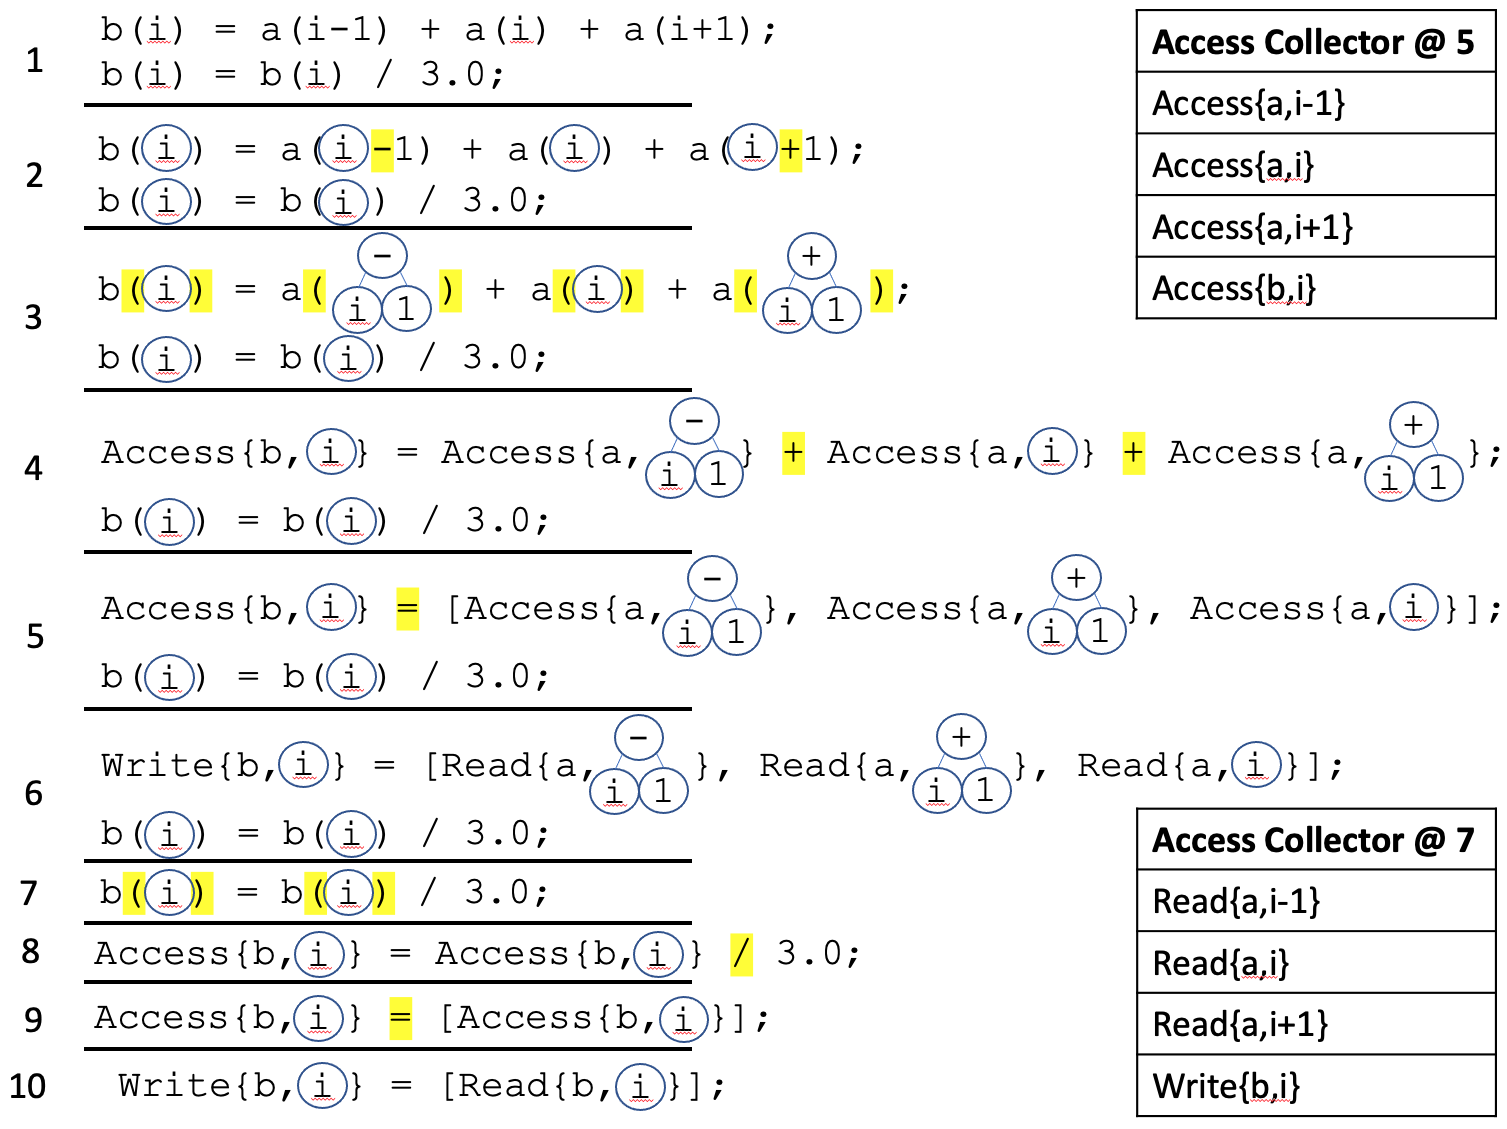
\includegraphics[width=\linewidth]{SymExecProcess.png}
\caption{Symbolic evaluation of a kernel lambda. 
Indexing expressions are evaluated first, then accesses, then statements in terms of accesses.
As assignments are evaluated, the accesses are marked as reads or writes.
Accesses are tracked using the access collector.}\label{symExec}
\end{figure}
Specifying parallelism within RAJA and other programming models can
build on commonly used abstractions such as \verb.forall..
However, determining when inter-loop scheduling transformations such as
loop fusion are legal requires an analysis of the dependences between those loops.
%Data access information is the largest missing piece for enabling loop chains
%in RAJA.
Other loop chain approaches require specification of data access patterns by
hand, which effectively rewrites the loop~\cite{bertolacci2019using}.
The symbolic evaluation mechanism eliminates this effort for the
developer by leveraging RAJA's array wrapping View abstraction.

%We leverage RAJA's array wrapping Views, which use the call operator to access
%arrays.
Using RAJA \verb.Views.,
an array access like \verb.a[i][j][k]. becomes the \verb.View. access \verb.a(i,j,k). as
Listing~\ref{symExecChanges} shows.
I overload the View function call operator with a symbolic iterator type to automate
data access pattern collection through symbolic execution.
%\todo{Brandon, by View call operator do you mean the overloaded parentheses?  Is that the terminology?} 
% yes: https://en.cppreference.com/w/cpp/language/operators#Function_call_operator
To use symbolic evaluation, kernel lambda arguments must be changed to
\verb.auto., which allows normal execution of lambda using index values while
its symbolical evaluation uses symbolic iterators.

Figure~\ref{symExec} shows the process of symbolically evaluating the body of a lambda. 
I break kernel symbolic evaluation into two contexts: indexing and accessing. 
Indexing encompasses the representation and storage of index expressions, like
\verb.i+1. in \verb.a(i+1)..
The symbolic evaluation must retain the entire structure of the index expression 
because the loop's
data access pattern must reflect the difference between \verb.a(i+1). and
\verb.a(i-1)..
Indexing evaluation is shown in steps 2 and 3 of Figure~\ref{symExec}.
Accessing encompasses the statement-level data access semantics of the kernels.
Unlike with indexing, only whether accesses are reads or writes matters,
not the entire structure of the statements.
For example, the analysis needs to know that the statement \verb.c(i) = a(i) + b(i).
reads \verb.a(i). and \verb.b(i). and writes \verb.c(i)., but not that it
adds \verb.a(i). and \verb.b(i)..
Access evaluation is shown in steps 4, 5, and 6 of Figure~\ref{symExec}.
Listing~\ref{ExpressionGrammar} shows the grammar for supported indexing expressions and access statements. 
Behavior for kernels that do not use this grammar is undefined.

Normal RAJA kernel execution only affects the states of its Views. 
However, symbolic evaluation should not change View states. 
Instead, it should only preserve the access information.
I achieve this by adding a class-wide access collector to the symbolic iterator. 
When symbolic accesses are evaluated, they are added to the collector, and updated as reads or writes when assignments are evaluated.
This access collector and its contents at steps 5 and 7 are shown to the right in Figure~\ref{symExec}, and the change can be seen between steps 5 and 6.


\begin{figure}[t]
\begin{lstlisting}[label={ExpressionGrammar},caption={EBNF Grammar to Support Symbolic Evaluation}]
start : Access Assignment Expression
Expression : Expression Operator Operand | Operand
Operand : Access | Int | Double | Iterator
Operator : + | - | * | / | %
Assignment : = | Update
Update: += | -= | *= | /= | %=

Access : Id '(' IndexExpressions ')'
IndexExpressions : IndexExpression | IndexExpression ',' IndexExpressions
IndexExpression : IndexOperand Operator IndexExpression | IndexOperand
IndexOperand : Int | Double | Iterator
\end{lstlisting}
\end{figure}
	
\subsection{Loop Chain Transformation Specifications}\label{sec:transspec}

With computation objects and their access patterns in hand, transformations can finally be applied.
RAJALC supports two transformations, loop fusion and overlapped tiling, each with two variants.
For all transformations, the user provides the target kernel
objects as arguments.
Listing~\ref{transformExample} shows two of these transformations in use.

Fusion transformations combine execution of iterations with the same iterator
values to improve data locality.
They work best for loops with producer-consumer relationships or those that
access the same data.
RAJALC's fusion transformations, \verb.fuse. and \verb.fuse_always., support
a tradeoff between safety and porting cost.
he former uses symbolic execution to determine if the transformation is legal.
The latter applies it prescriptively.
If the user knows the dependences between loops do not impede fusion,
it allows them to fuse kernels that do not use Views. 
On the other hand, \verb.fuse. requires the user to use Views instead
of arrays to limit the fusion transformation to when it is safe.

Overlapped tiling transformations improve data locality
and enables parallelism by performing some redundant computation 
on the surface of the tiles.
They work best for loops with stencil-like access patterns,
where fusion results in a more restricted wavefront parallelism.
RAJALC's two overlapped tiling transformations, \verb.overlapped_tile. and
\verb.overlapped_tile_fuse., differ in the execution schedule within each tile
as Figures~\ref{tileNofuse} and~\ref{tileFuse} show.
Specifically, the schedule within the tile of \verb.overlapped_tile. mimics
a sequential schedule by executing all iterations of the first kernel before
it executes all iterations of the second while \verb.overlapped_tile_fuse.
fuses individual iterations of the loops within each tile.
Lines 11 through 21 of Listing~\ref{transformExample} show how to use these transformations.

When using the \verb.fuse. variant or either overlapped tiling transformation, if analysis shows the transformation to be unsafe, a warning message is printed and the original schedule is used. 

\subsection{Compile- and Run-time Actions}

When the programmer uses a RAJALC loop transformation, the compiler instantiates two different executor types for the entire loop chain. 
The first executor uses the transformed schedule, while the second uses the original schedule. 
Both executors are included with the object returned by the transformation call.

At run-time, when each kernel is initialized, its data access patterns are collected and cached. 
This reduces the cost of the symbolic evaluation by only performing it once, even through kernels are typically executed many times.
Then, the access information is used by the transformation functions to select which schedule should be used.


\begin{figure*}
	\centering

	\begin{subfigure}[t]{0.45\textwidth}
		\centering
		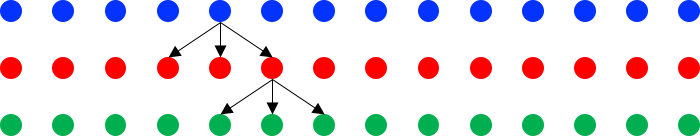
\includegraphics[height=0.45in]{TilingProcess/TilingProcess1.png}
		\caption{Original kernel iteration spaces and abbreviated dependences between iterations.}\label{tiling1}
	\end{subfigure}
	~
	\begin{subfigure}[t]{0.45\textwidth}
		\centering
		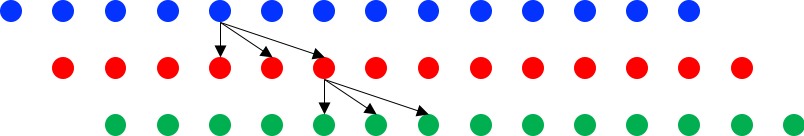
\includegraphics[height=.45in]{TilingProcess/TilingProcess2.png}
		\caption{After shifting kernels to remove negative dependences.}\label{tiling2}
	\end{subfigure}
	\par\bigskip
	\begin{subfigure}[t]{0.45\textwidth}
		\centering
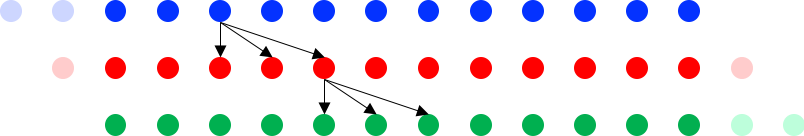
\includegraphics[height=0.45in]{TilingProcess/TilingProcess3.png}
		\caption{Shared iteration space. Chain could be fused sequentially.}\label{tiling3}
	\end{subfigure}
	~
	\begin{subfigure}[t]{0.45\textwidth}
		\centering
		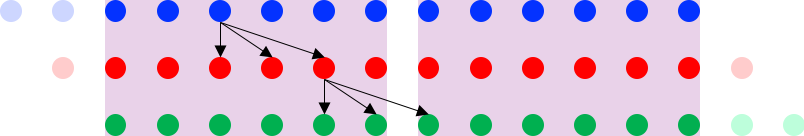
\includegraphics[height=.45in]{TilingProcess/TilingProcess4.png}
		\caption{Underlying tiles for TileSize=6 shaded in purple.}\label{tiling4}
	\end{subfigure}
	\par\bigskip
	\begin{subfigure}[t]{0.45\textwidth}
		\centering
		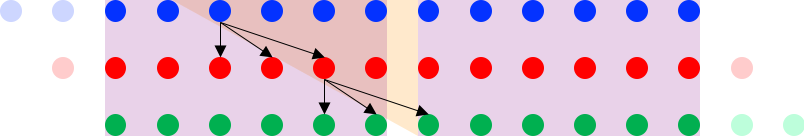
\includegraphics[height=0.45in]{TilingProcess/TilingProcess5.png}
		\caption{Overlap for each tile shaded in orange. Tiles against low edge have no overlap.}
	\end{subfigure}
	~
	\begin{subfigure}[t]{0.45\textwidth}
		\centering
		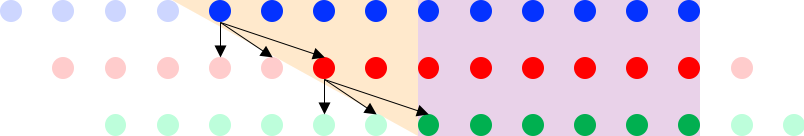
\includegraphics[height=.45in]{TilingProcess/TilingProcess6.png}
		\caption{An individual overlapped tile.}
	\end{subfigure}
	\par\bigskip
	\begin{subfigure}[t]{0.45\textwidth}
		\centering
		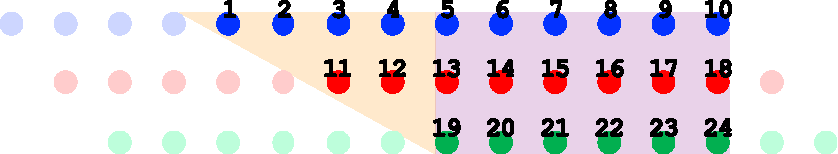
\includegraphics[height=0.45in]{TilingProcess/TilingProcess7.pdf}
		\caption{Execution order for an individual tile without fusion.}\label{tileNofuse}
	\end{subfigure}
	~
	\begin{subfigure}[t]{0.45\textwidth}
		\centering
		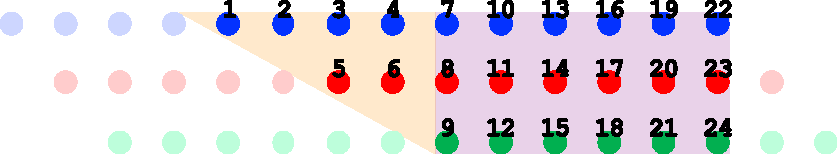
\includegraphics[height=0.45in]{TilingProcess/TilingProcess8.pdf}
		\caption{Execution order for an individual tile with fusion.}\label{tileFuse}
	\end{subfigure}
	\par\bigskip
	\begin{subfigure}[t]{\textwidth}
		\centering
		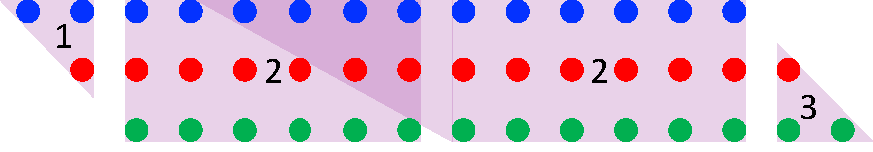
\includegraphics[height=0.45in]{TilingProcess/TilingProcess9.pdf}
		\caption{Global execution order for entire computation.}\label{tiling9}
	\end{subfigure}

\caption{Overlapped tiling of 3 one-dimensional loops.}\label{tilingProcess}
\end{figure*}

\section{Transformations Safety in RAJALC}
Section~\ref{sec:transspec} shows how a user can specify the use of loop fusion transformations
or overlapped and fusion transformations on loops in a chain.
In this section, I describe 
how RAJALC generates different execution schedules and uses the information gathered from the symbolic evaluation to verify their correctness.

\subsection{Loop Shifting for Stencil Computations}

While \verb.fuse_always. prescriptively apples a fusion transformation
without checking its legality, \verb.fuse. uses symbolic evaluation to
guide a legal loop fusion.
For a fusion to be legal, the inter-loop dependences cannot have a
negative direction.
However, loops can often be shifted to make such
dependences non-negative.
Figures~\ref{tiling1} and~\ref{tiling2} show an example of shifting the
loops to adjust negative dependences.
Prior work showed how to convert the dependence relations into constraints
of an ILP optimization problem~\cite{bertolacci2019using}.
RAJALC minimizes the sum of the non-negative shift amounts
$S_{1,1},S_{1,2},\ldots,S_{2,1},\ldots,S_{l,n}$ with the constraints $S_{b,i} + d_i \geq S_{a,i}$ for each dependence
$[d_1,d_2,\ldots,d_n]$ from kernel $a$ to $b$.
Solutions to this problem correspond to shift amounts that enable loop fusion.
RAJALC also use this shifting mechanism to simplify the dependences for overlapped
tiling.

While fusion in this circumstance improves data locality, it restricts
parallelism.
Because fusion combines iterations of different loops, dependences that
are originally between different loops become dependences between iterations
of the same loop. 
While wavefront parallelism may still be possible, overlapped tiling often
offers a better balance of parallelism and data locality~\cite{CathieSC14}.

\subsection{Iteration Space Alignment and Lambda Generation}
When performing optimizing transformations, kernel iteration spaces do not
always completely align. 
Misalignments can arise from differences in the original iteration spaces
or from shifts to remove negative dependences. 
While the iterations the loops in a chain have in common are executed by
the fused or tiled kernels, we also must generate extra kernels to execute
the unshared boundary iterations.

Figure~\ref{fusionPartition} illustrates the generation of these kernels
for one $d=3$ loop in a chain. 
First, RAJALC calculates the shared iteration space of the chain, using the
intersection of all kernel iteration spaces, which yields a $d$-dimensional
hyper-rectangle within each kernel's iteration space, as
Figure~\ref{sharedSpace} shows.
To account for the boundary iterations, RAJALC then partitions the loop's
iteration space, using the faces of the shared iteration space.
Figures~\ref{preshare} and~\ref{postshare} show the iteration spaces of the
$2*d=6$ boundary kernels for the 3D loop. 
This process generates $2*d*n$ boundary kernels across the $n$ loops in a
chain, plus the one fused/tiled kernel over the shared iteration space. 
RAJALC orders these $2*d*n+1$ kernels by loop and dimension to execute the low
boundary iterations, the shared iterations, then the high boundary iterations.

Each kernel requires an iteration space and a lambda describing the loop body. 
For the boundary iterations, RAJALC uses the original lambdas. 
For the shared iterations, a new lambda is generated based on the transformation. 
With fusion, the new lambda executes the sequence of original lambdas, performing one iteration of each loop.
With overlapped tiling, the new lambda executes each original lambda across its share of the tile, as shown in Figure~\ref{tileNofuse}.


\begin{figure}
	\captionsetup[subfigure]{justification=centering}
		\centering
		\begin{subfigure}[t]{0.33\textwidth}
			\centering
			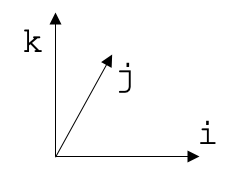
\includegraphics[height=0.5in]{FusionPartition/axes.png}
			\caption{Dimension order of loop.}
		\end{subfigure}
		
	%	\begin{subfigure}[t]{0.33\textwidth}
	%		\centering
	%		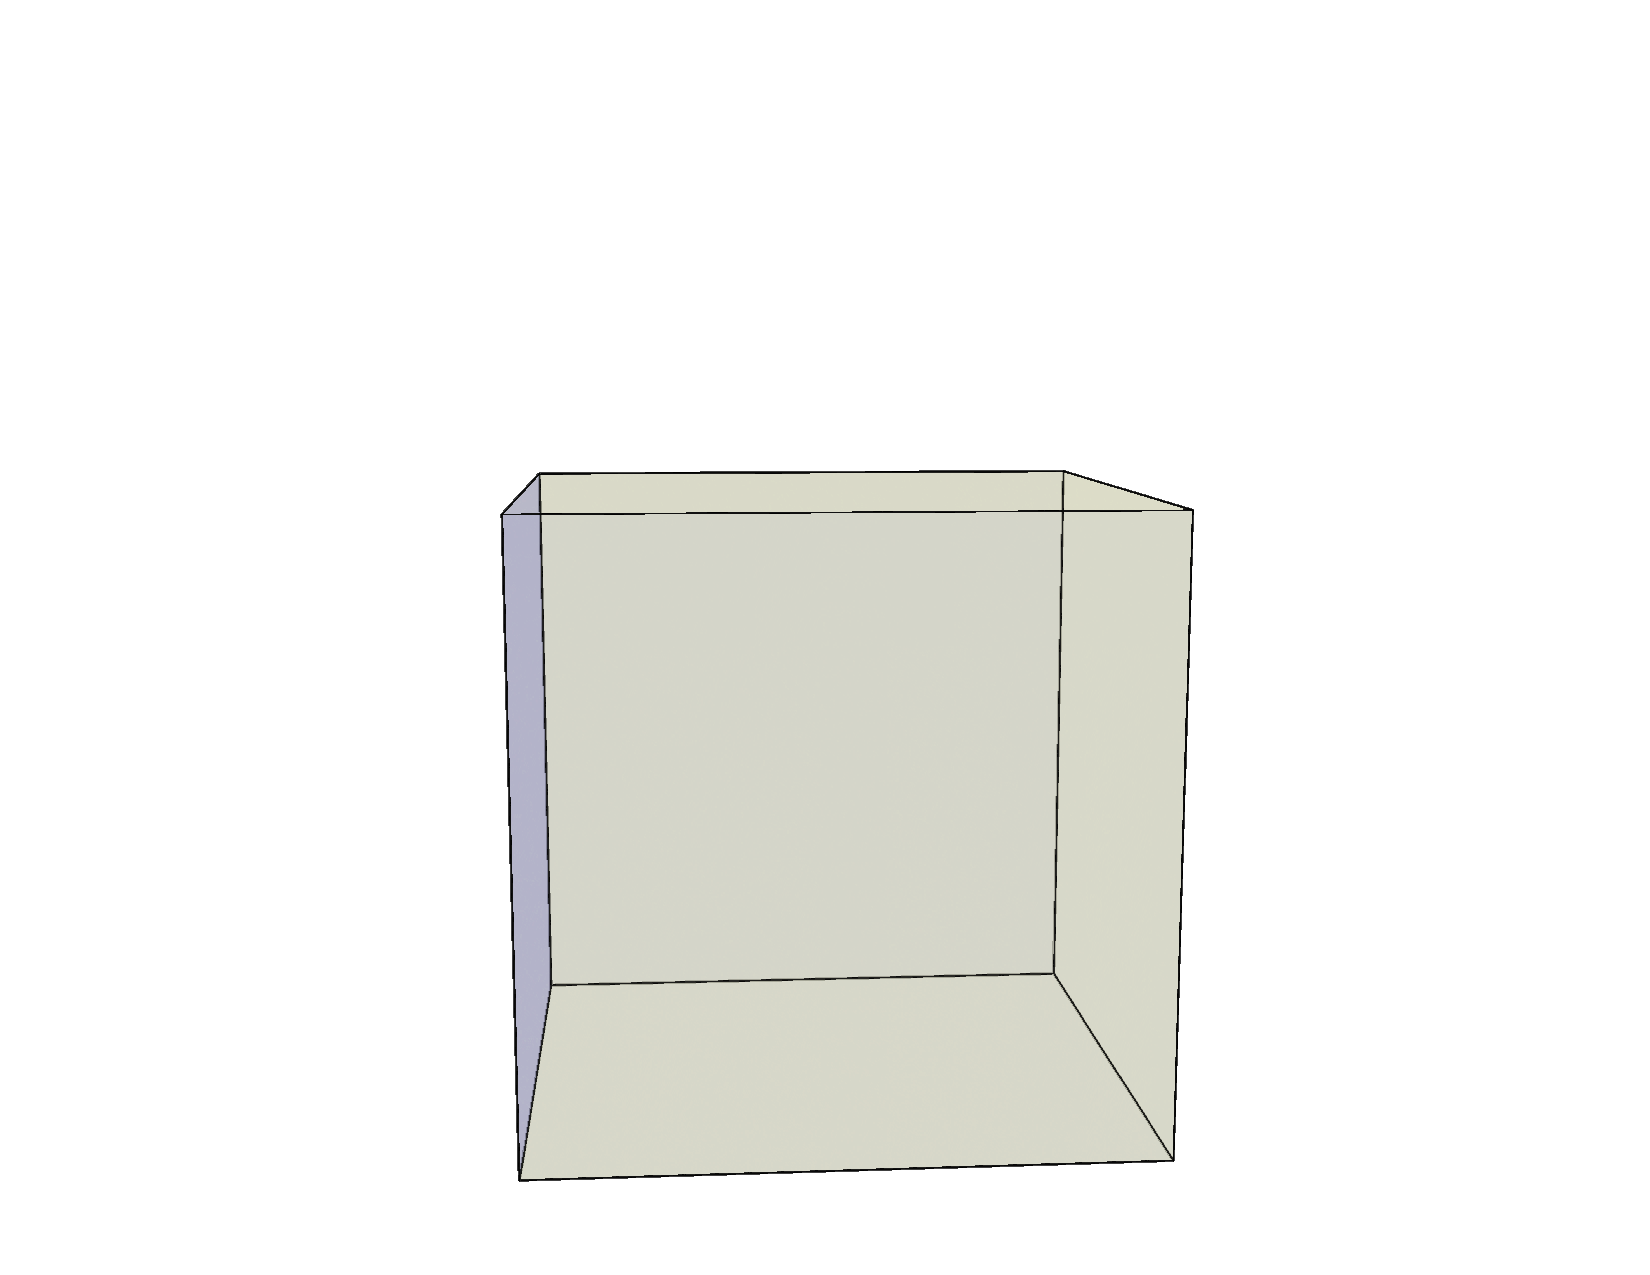
\includegraphics[height=1.5in, clip=true, trim=200 0 200 200]{FusionPartition/FusionPartition1.pdf}
	%		\caption{Original iteration space of one loop in chain.}
	%	\end{subfigure}
		
		\begin{subfigure}[t]{0.45\textwidth}
			\centering
			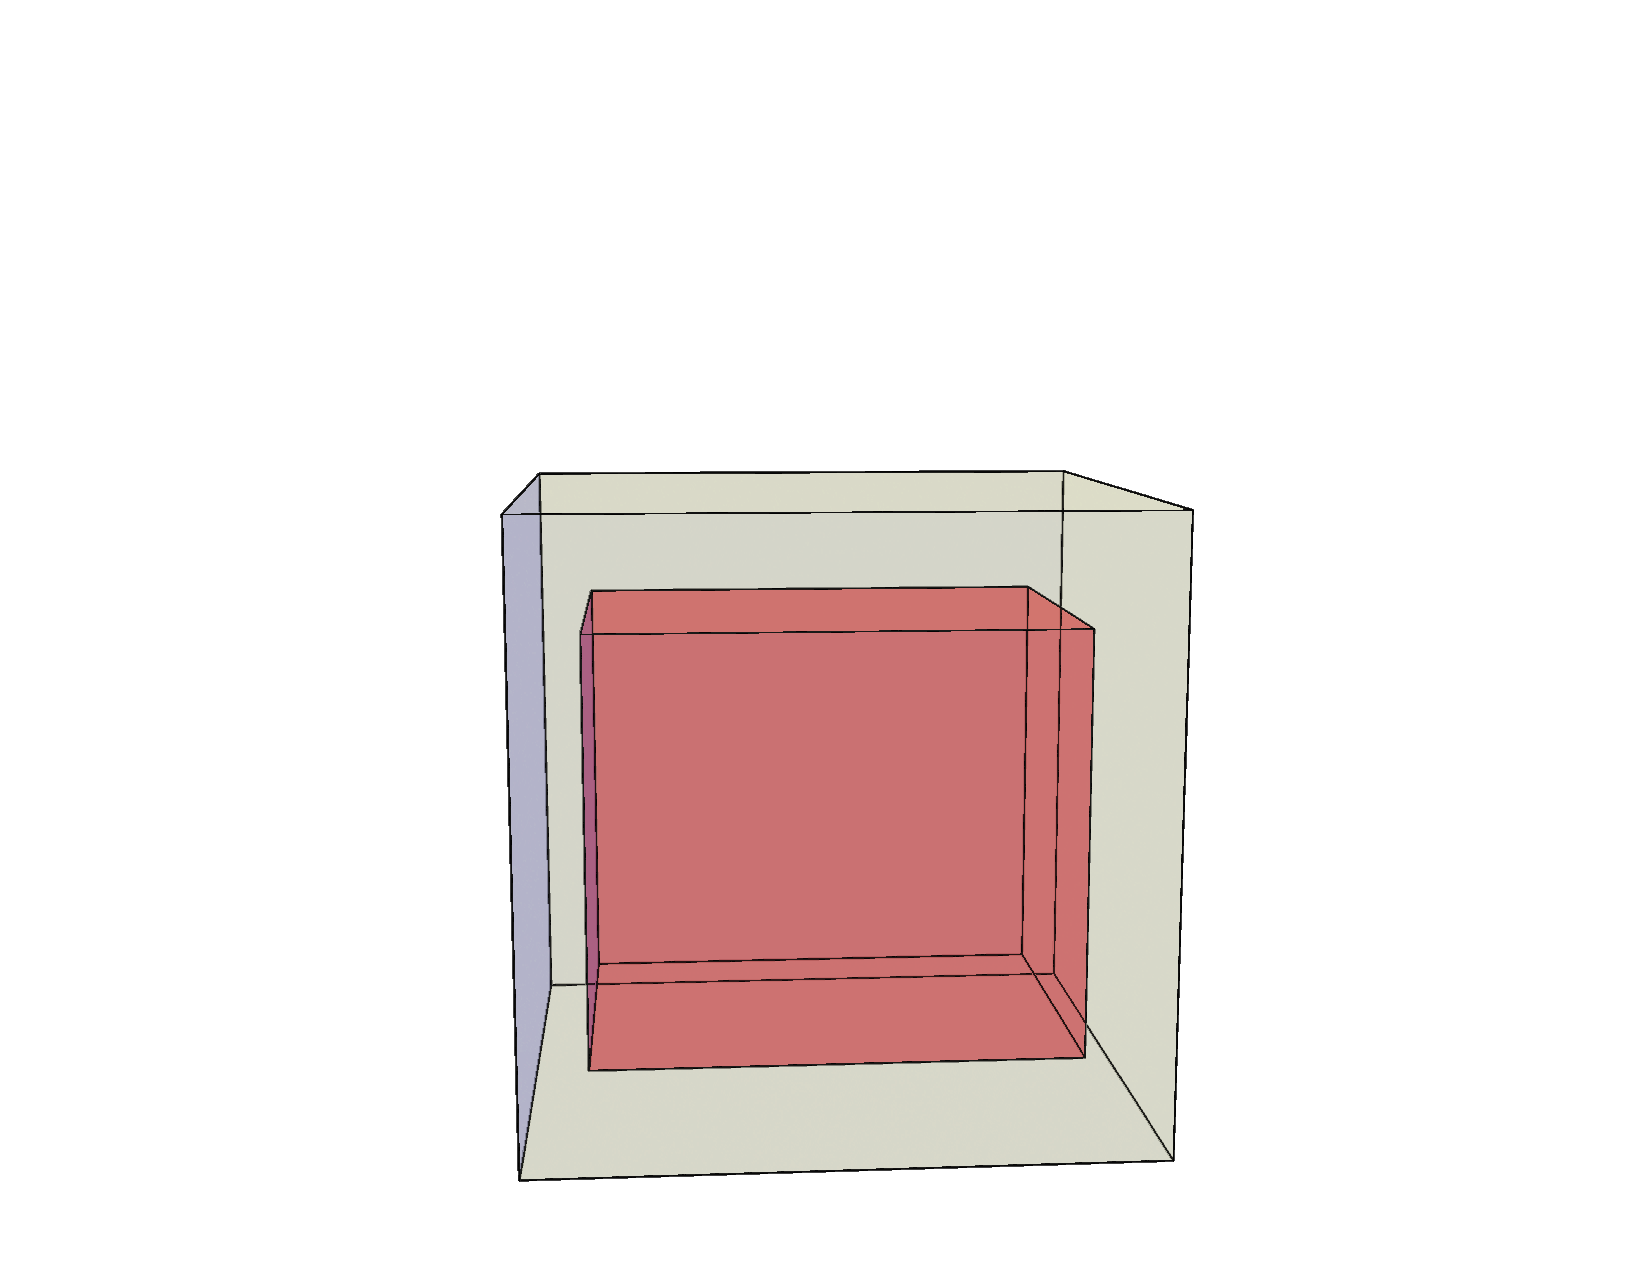
\includegraphics[height=1.5in, clip=true, trim=200 20 200 200]{FusionPartition/FusionPartition2.pdf}
			\caption{Original iteration space of one \\ loop in chain and shared iteration \\ space executed by fused kernel.}\label{sharedSpace}
		\end{subfigure}
		\begin{subfigure}[t]{0.45\textwidth}
			\centering
			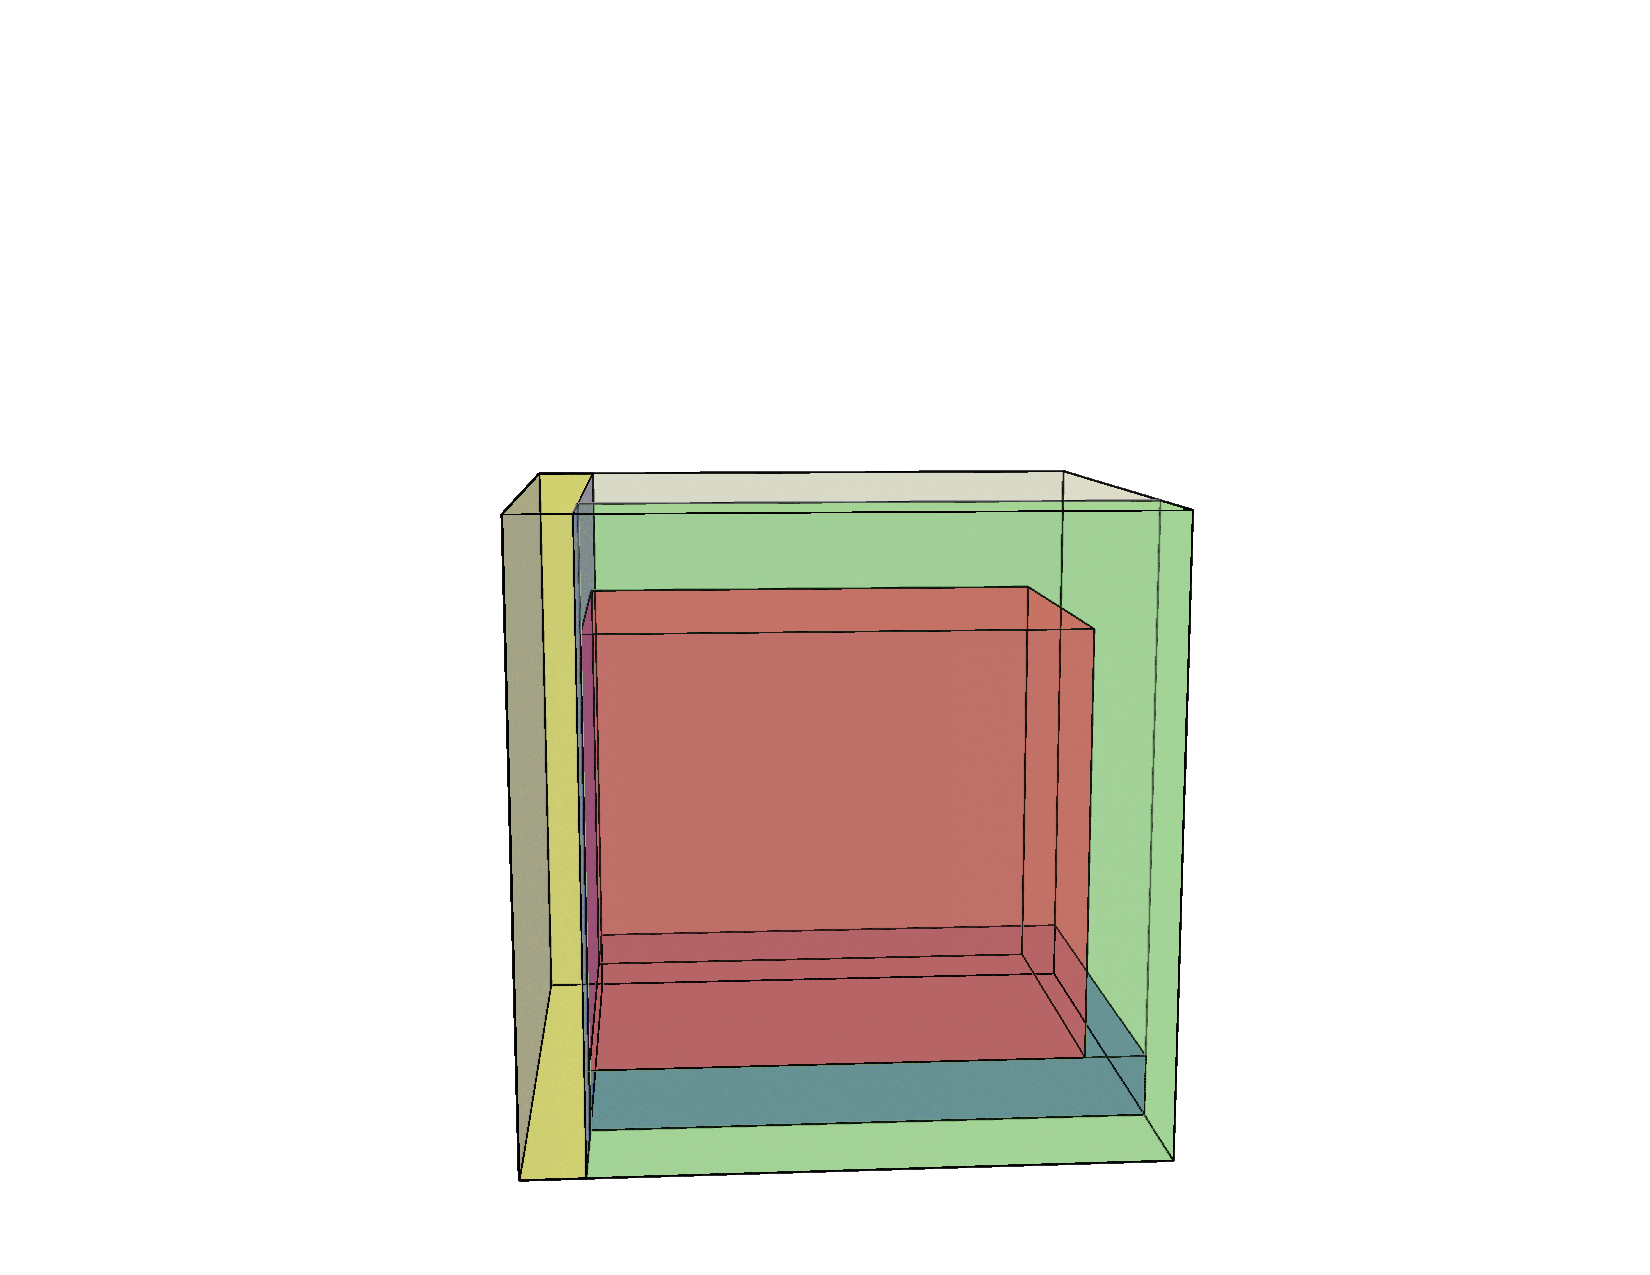
\includegraphics[height=1.5in, clip=true, trim=200 20 200 200]{FusionPartition/FusionPartition5.pdf}
			\caption{Lower boundary iteration spaces.}\label{preshare}
		\end{subfigure}
	
		\begin{subfigure}[t]{0.5\textwidth}
			\centering
			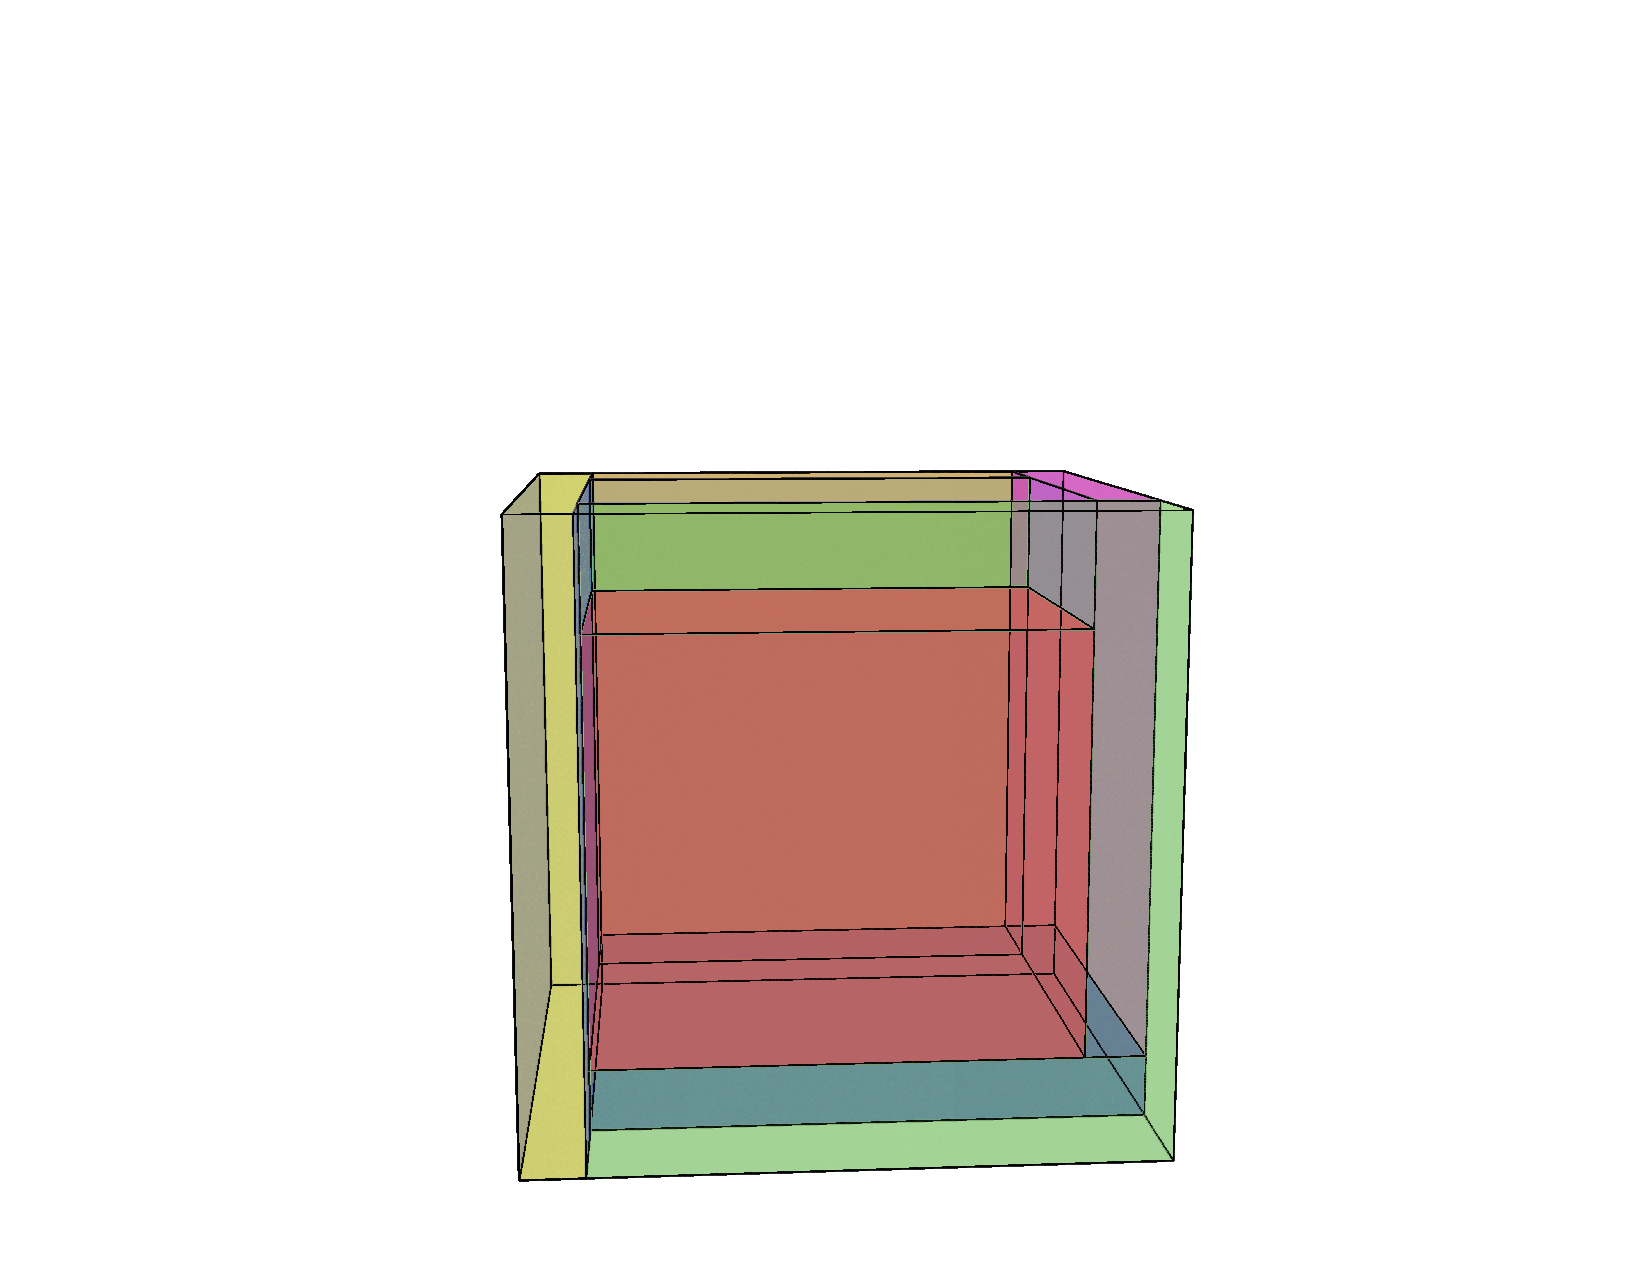
\includegraphics[height=1.5in, clip=true, trim=200 20 200 200]{FusionPartition/FusionPartition8.pdf}
			\caption{Higher boundary iteration spaces.}\label{postshare}
		\end{subfigure}
	\caption{Partitioning the iteration space of a single 3d loop. The original iteration space is $(0,10)\times(0,10)\times(0,10)$ and the fused iteration space is $(1,9)\times(2,8)\times(1,8)$. This partitioning process occurs for each kernel in the chain.}\label{fusionPartition}
	\end{figure}
	


\subsection{Overlapped Tiling}

Overlapped tiling proceeds similarly to the \verb.fuse. transformation. 
First, RAJALC calculates and applies shifts to remove negative dependences as
Figures~\ref{tiling1} and~\ref{tiling2} show.
Next, it calculates the overlapping iteration space and partition boundary
iterations as Figure~\ref{tiling3} shows.
Finally, it perform overlapped tiling as Figures~\ref{tiling4}-\ref{tiling9} show.

Before RAJALC can generate the kernel for the overlapped tiling, it must
calculate the overlap amounts. 
This is set up as an ILP optimization problem similarly to the calculation of the
shift amounts.
For $n$ kernels of dimension $m$, the optimization problem is over the $nm$
overlap amounts $O_{1,1},O_{1,2},\ldots,O_{2,1},\ldots,O_{n,m}$.
I introduce a non-negativity constraint to ensure that all overlap amounts
are greater than zero. 
I then add the constraints
$O_{a,1} >= O_{b,1} + d_{1}, O_{a,2} >= O_{b,2} + d_{2},\ldots,O_{a,m} >= O_{b,m} + d_{m}$
for each dependence $D=[d_{1},d_{2},\ldots,d_{m}]$ from kernel $a$ to kernel $b$,
which ensures that if a tile includes an iteration of kernel $b$, it also
includes all necessary iterations of kernel $a$.
Finally, it minimizes the sum of the overlap amounts
$\sum_{i=1}^{n} \sum_{j=1}^{m} O_{i,j}$.

After RAJALC calculates the overlap amounts, it generates a kernel that iterates
over each tile, executing the original kernels for the iterations of the tile.
The two overlapped tiling transformations, \verb.overlapped_tile_no_fuse.
and \verb.overlapped_tile_fuse. differ in their schedule for executing each
tile.
Without fusion, it executes the tile one kernel at a time: all of $knl1$ is
executed, then all of $knl2$, and so on. 
tile sizes are constrained for this schedule by cache size and by the size of
the overlap. 
Tiles must be small enough to fit into cache to maximize data locality
benefits, but tile size should be maximized to reduce the proportion of
recomputation.

In contrast, the \verb.overlapped_tile_fuse. transformation fuses iterations
within each tile using the fusion algorithm described above.
Introducing fusion into the tile decouples data locality from cache size.
Unrestricted by cache considerations, the only limit on tile size is the
need for parallelism, enabling larger tiles than otherwise possible.

\section{Case Study: RAJA Performance Suite}

I evaluate the advances through two case studies, porting the RAJA
Performance Suite (RAJAPerf)~\cite{hornung2017raja} and LULESH from
standard RAJA to RAJALC\@
In both case studies, I evaluate the performance and porting process
of the RAJALC implementations and I detail benefits and limitations
of the approach.

The RAJA Performance Suite is a collection of benchmark kernels that are
used to evaluate RAJA performance.
The suite contains 46 benchmark kernels across five categories; 33 contain
a single loop nest, leaving 13 kernels for which the advances are relevant.
Four of these are matrix computations involving reductions to which 
RAJALC's current capabilities do not apply. 
Finally, one benchmark does not exhibit any data reuse, so no data locality 
optimizations are relevant, including those supported here. 
Thus, I evaluate RAJALC on 8 benchmark kernels.

For each of the 8 kernels, I identify a locality-improving transformation
and implement new variants.
The first variant, \verb.Hand_Opt., applies the transformations directly.
The second variant, \verb.LoopChain., applies the transformation using RAJALC\@.
I record the number of modified or added source lines of code for each
variant and evaluate their performance on three systems.
%Rose
System Intel1 has an 8-core Intel Core i7--6900K CPU at 3.2 GHz and 32G of memory.
% 512K L1 cache, 2M L2 cache, and 20M L3 cache.
It runs Ubuntu 16.04.7 and GCC11.0.
%Quartz
System Intel2 has a 36-core Intel Xeon E5--2695 CPU at 2.1 GHz and 128 GB of memory.
%Lassen
System Power9 has an 44-core IBM Power9 at 3.5 GHz and 256 GB of memory.
Systems Intel2 and Power9 run TOSS 3 and GCC8.3.1.


\subsection{Benchmark Descriptions}

I categorize each benchmark as either point-wise or stencil. 
Point-wise loops access at most one element of each array per iteration,
while stencil loops access a fixed pattern of elements of each array per
iteration. 
The loop bodies
\verb.lambda1. and \verb.lambda2. in Listing~\ref{transformExample} are
examples of point-wise loops, while \verb.lambda3. and \verb.lambda4. are
examples of stencil loops.

Three of the benchmarks, \verb.GEN_LIN_RECUR., \verb.ENERGY., and
\verb.PRESSURE., are point-wise computations.
\verb.GEN_LIN_RECUR. comes from a general linear recurrence computation and
\verb.ENERGY. and \verb.PRESSURE. are loops extracted from LULESH, a
hydrodynamics code. 
For these benchmarks, loop fusion does not interfere with parallelism, so
I apply that transformation.

The other five benchmarks are stencil computations: \verb.JACOBI_1D.,
\verb.JACOBI_2D., \verb.HEAT_3D., \verb.HYDRO_2D., and \verb.FDTD_2D..
\verb.JACOBI_1D., \verb.JACOBI_2D., and \verb.HEAT_3D. compute solutions
to discretized PDEs in their respective dimensions.
\verb.HYDRO_2D. is part of a hydrodynamics code.
\verb.FDTD_2D. is a finite-difference time-domain kernel that is unique
among the stencil computations because I can fuse two of its four loops 
without inhibiting parallelism.
Thus, I apply that transformation.
The other four require shifting to be fused, so I apply overlapped tiling
to retain sufficient parallelism.

\subsection{Porting}

Implementing the fusion transformation is fairly easy. 
For the RAJALC variant, because I can confirm their point-wise nature
visually, symbolic evaluation is unnecessary.
Thus, I directly apply the transformation without converting the kernels to 
RAJA Views.
The hand-applied variant code changes are also low impact; in a real
application they would not be desirable as the kernels may be used separately
in other contexts.
Instead of multiple calls to \verb.RAJA::kernel. with the different loop
bodies, a single call is made with all loop bodies as one.
For the \verb.GEN_LIN_RECUR. benchmark, I also apply a loop reversal
transformation by hand to both variants. RAJALC does not currently support 
loop reversal, but its inclusion in the implementation would not be difficult.
However, automation of its use and its limited applicability in 
existing RAJA applications has made its implementation low priority. 

For \verb.HYDRO_2D., applying overlapped tiling transformation with RAJALC 
requires minimal changes: I add two lines of code and change three. 
In contrast, the hand implementation changes four lines and added 41
new lines, effectively an order of magnitude more effort. 
These additional lines calculate the amounts to shift and to overlap, 
create the new, tiled kernel, and execute the boundary iterations not
within the tiled area. 
These changes are not simple; the porting process encountered errors
in nearly all parts: shifting, boundary iterations, tile sizes, tile
bounds, and tile execution.

Porting effort in source lines of code
for the other three overlapped tiling kernels is similar to 
\verb.HYDRO_2D., with one major difference.  
While \verb.HYDRO_2D. has distinct input and output arrays; \verb.JACOBI_1D., 
\verb.JACOBI_2D., and \verb.HEAT_3D. each use one of two arrays for
input and output, which introduces anti-dependences that inhibit 
overlapped tiling. 
To mitigate this effect, I modify the kernels to use
a double-buffer strategy that eliminates the anti-dependence. 
Listing~\ref{jacobiDoubleBuffer} shows the double-buffer reference
implementation for \verb.JACOBI_1D..
%%
I add the double-buffer transformation by hand in these three variants;
its automation is future work.
I plan to use the access information collected during symbolic evaluation
to identify chains that require it and to implement the double buffer within
the View class.
\begin{figure}[t]
\begin{lstlisting}[label={jacobiDoubleBuffer},caption={Double-Buffer Implementation for JACOBI\_1D}]
for(int t = 0; t < numIters; t++) {
	temp = A1.data_ptr;
	A1.data_ptr = A2.data_ptr;
	A2.data_ptr = temp;
	for(int i = 0; i < length; i++) {
		B(i) = 0.33333 * (A1(i-1) + A1(i) + A1(i+1));
	}
	for(int i = 0; i < length; i++) {
		A2(i) = 0.33333 * (B(i-1) + B(i) + B(i+1));
	}
}
\end{lstlisting}
\end{figure}

Table~\ref{sloc} shows the number of changed and added source lines of code
for all benchmarks.
Overall, manual porting difficulty in source lines of code 
increases as the dimensionality of a 
kernel increases, mostly due to the specification of the boundary iterations. 
Alternatively, RAJALC porting difficulty is similar regardless of the loop
dimensionality.
Also, while with RAJALC code retains its original structure, the 
hand-implemented transformations obscure the underlying computation,
which significantly complicates code maintenance.
\begin{table}[t]
\begin{tabular}{|l|l|l|l|l|}
\hline
\textbf{Benchmark}       & \multicolumn{2}{l|}{\textbf{\begin{tabular}[c]{@{}l@{}}Manual \\ Implementation\end{tabular}}} & \multicolumn{2}{l|}{\textbf{\begin{tabular}[c]{@{}l@{}}RAJALC\\ Implementation\end{tabular}}} \\ \hline
\cellcolor[HTML]{9B9B9B} & Changed                                         & Added                                        & Changed                                        & Added                                        \\ \hline
\textit{ENERGY}          & 6                                               & 6                                            & 6                                              & 2                                            \\
\textit{PRESSURE}        & 2                                               & 3                                            & 2                                              & 2                                            \\
\textit{GEN\_LIN\_RECUR} & 1                                               & 1                                            & 2                                              & 2                                            \\
\textit{FDTD\_2D}        & 8                                               & 4                                            & 9                                              & 4                                            \\
\textit{HYDRO\_2D}       & 4                                               & 41                                           & 3                                              & 2                                            \\
\textit{JACOBI\_1D}      & 3                                               & 17                                           & 3                                              & 3                                            \\
\textit{JACOBI\_2D}      & 10                                              & 33                                           & 10                                             & 3                                            
\\
\textit{HEAT\_3D}        & 12                                              & 38                                           & 12                                             & 3                                            \\ \hline
\textit{Average}        & 5.8                                              & 17.9                                           & 5.9                                            & 2.6                                            \\ \hline
%\textit{Average}        & 5.75                                              & 17.875                                           & 5.875                                            & 2.625                                            \\ \hline
\end{tabular}
\caption{Lines of Code Impact (Excludes double-buffer transformation changes)}\label{sloc}
\end{table}

\subsection{Performance}
\begin{figure}
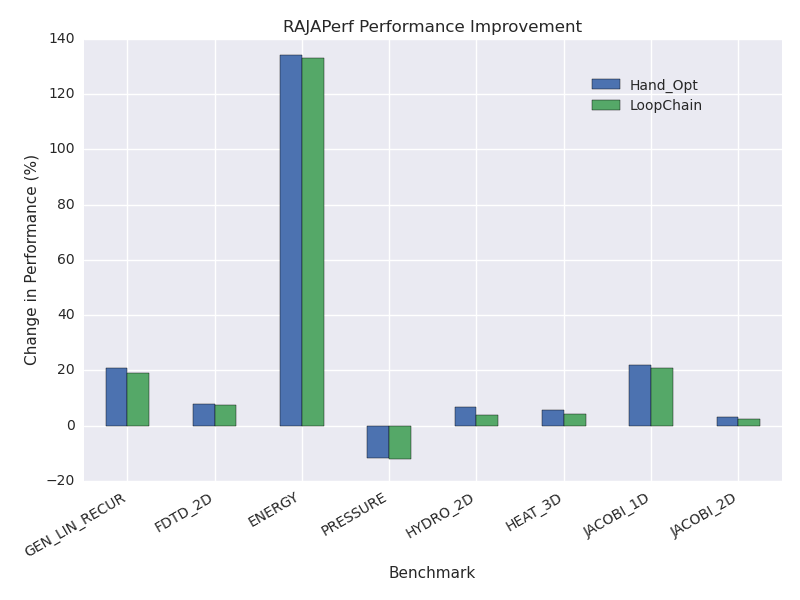
\includegraphics[width=\linewidth]{results/RajaPerf/Rose/RAJAPerf.png}
\caption{Performance changes of RAJAPerf benchmarks on System Intel1 (higher is better).}\label{RAJAPerfPerf}
\end{figure}
Figure~\ref{RAJAPerfPerf} shows the performance of the hand-implemented
and RAJALC variants relative to the original implementations on System Intel1. 
For the double-buffer implementations, I show the performance relative to an 
un-transformed double-buffer implementation. 
I report the average of ten runs. 

For the fused benchmarks, \verb.GEN_LIN_RECUR. and \verb.FDTD_2D. improve
modestly while \verb.PRESSURE. performance drops slightly, likely due to low amounts of data reuse. 
\verb.ENERGY. runs more than two times faster than the original, likely due
to the larger number of fused kernels than the other benchmarks. 
For all four, the RAJALC variant's performance is comparable to the
hand-implemented loop fusion. 
 
For the overlapped tiled benchmarks, the \verb.Hand_Opt. variant improves
performance up to 22\% for all benchmarks.
The RAJALC variant, which achieves its best performance with different tile sizes, improves performance by 
up to 20\%.
For both variants, the tile sizes were tuned manually.
Overall, the RAJALC variant achieves 85\% of the geometric mean performance
improvement of the hand-implemented variant. 


Because of the large thread counts on Systems Intel2 and Power9, I evaluated the scaling performance of RAJAPerf when using RAJALC\@.
Unlike on System Intel1, RAJAPerf often did not benefit from the inter-loop
optimizations on Systems Intel2 and Power9, even when applied by hand. 
However, the direction of RAJALC's performance impact was nearly identical to the hand-optimized code. 
On System Intel2, 47 of the 48 benchmark-thread-count combinations had the same direction of impact.
On System Power9, all 48 combinations matched the direction of performance impact between the two variants.
Overall, the geometric mean of the fraction of the hand-implemented speedup achieved by RAJALC ranges across thread counts from 0.92 and 0.97 on System Intel2 and 0.95 and 1.02 on System Power9. 
This is evidence that RAJALC is a useful tool for quickly prototyping transformations without large refactoring costs and accurately recreates the performance impact of hand implementing the transformations.

\section{Case Study: LULESH}

While the RAJAPerf case study demonstrates the types of computations RAJALC
can optimize, the second case study, LULESH, explores its potential within a
larger application.
LULESH is a DOE proxy application for shock hydrodynamics codes.
It solves a simple Sedov blast problem using the typical numerical algorithms and computational characteristics for larger codes.

As with the previous case study, I characterize the porting process and
evaluate RAJALC performance compared to the original implementation.
For this evaluation, I ported LULESH v2.0~\cite{LULESH2}. 

\subsection{Porting}

Porting LULESH is more involved than the RAJAPerf kernels. 
I must first identify the part of the application to optimize,.
I choose the function \verb.EvalEOSForElems., which has a long series
of point-wise computations over the same iteration space.
The \verb.ENERGY. and \verb.PRESSURE. benchmarks within RAJAPerf are
from this part of LULESH\@.

\subsubsection{Code Change: Arrays to Views}

The RAJA implementation of LULESH uses RAJA execution statements, but
does not use RAJA Views for arrays and vectors. 
Thus, I first convert these data structures to use Views.
For many of the data structures, array accesses are abstracted through
indexing functions. 
I replace these indexing functions directly with Views without changing
the source code of the algorithms.
However, the existing version often uses arrays, especially for local and
temporary storage.
I wrap these arrays with Views and change the accesses from brackets to
parentheses, a tedious but simple code change.

\subsubsection{Code Change: Kernel Objects}

The second required change uses RAJALC kernel objects instead of direct
code execution.
I move the series of point-wise computations in \verb.EvalEOSForElems. that operate over the same iteration space into many individual functions.
I modify them to create and to return the kernel objects, which allows us
to fuse them, both by hand and with RAJALC\@.


\subsubsection{Challenge: Indirect Accesses}
The \verb.nodelist. function, which creates a list of indices for the area
around an element, poses a challenge to the LULESH porting.
Because this function takes the loop index and returns a list of indices,
it interferes with symbolic evaluation.
RAJALC has similarities to inspector-executor strategies commonly used when optimizing sparse codes, which may provide some direction in attempts to optimize RAJA-based sparse codes. 

\subsubsection{Challenge: Non-contiguous Iteration Spaces}

LULESH is an unstructured application: its iteration spaces are collections
of ranges instead of contiguous ranges. 
For example, instead of iterating over every value from 0 to 100, it may
iterate over values 0 to 10, then 17 to 23, then 52, 73, and 75 to 100.
RAJALC currently only handles contiguous iteration spaces, so it only
applies fusion to LULESH problems that use contiguous ranges.
In practice, this limitation is a benefit over hand optimizations that assume
such ranges.
Nonetheless, the prevalence of unstructured scientific applications makes
fusion of unstructured ranges a valuable future research direction.


\subsection{Performance}

WIe evaluate the performance of three LULESH variants: Original, RAJALC, and
By Hand.
Original is the original v2 RAJA implementation.
RAJALC is the version ported to apply loop fusion with RAJALC while By Hand
directly applies loop fusion by hand.


\begin{figure}[t]
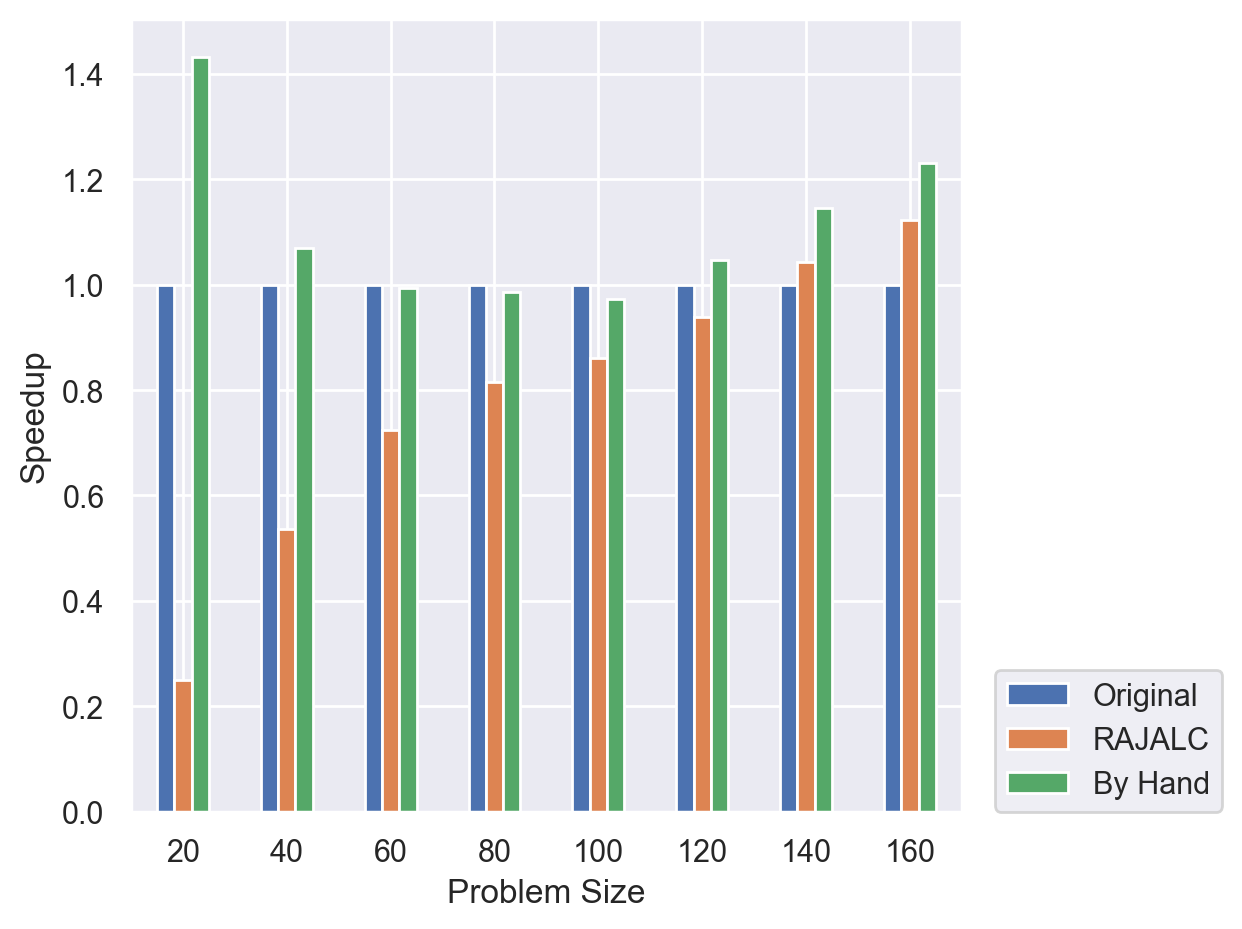
\includegraphics[width=\linewidth]{results/Lulesh/LuleshRoseGcc8All/LuleshRoseGcc8All.png}
\caption{LULESH Speedup on System Intel1 (higher is better).}\label{LULESHRose}
\end{figure}

\begin{figure}[t]
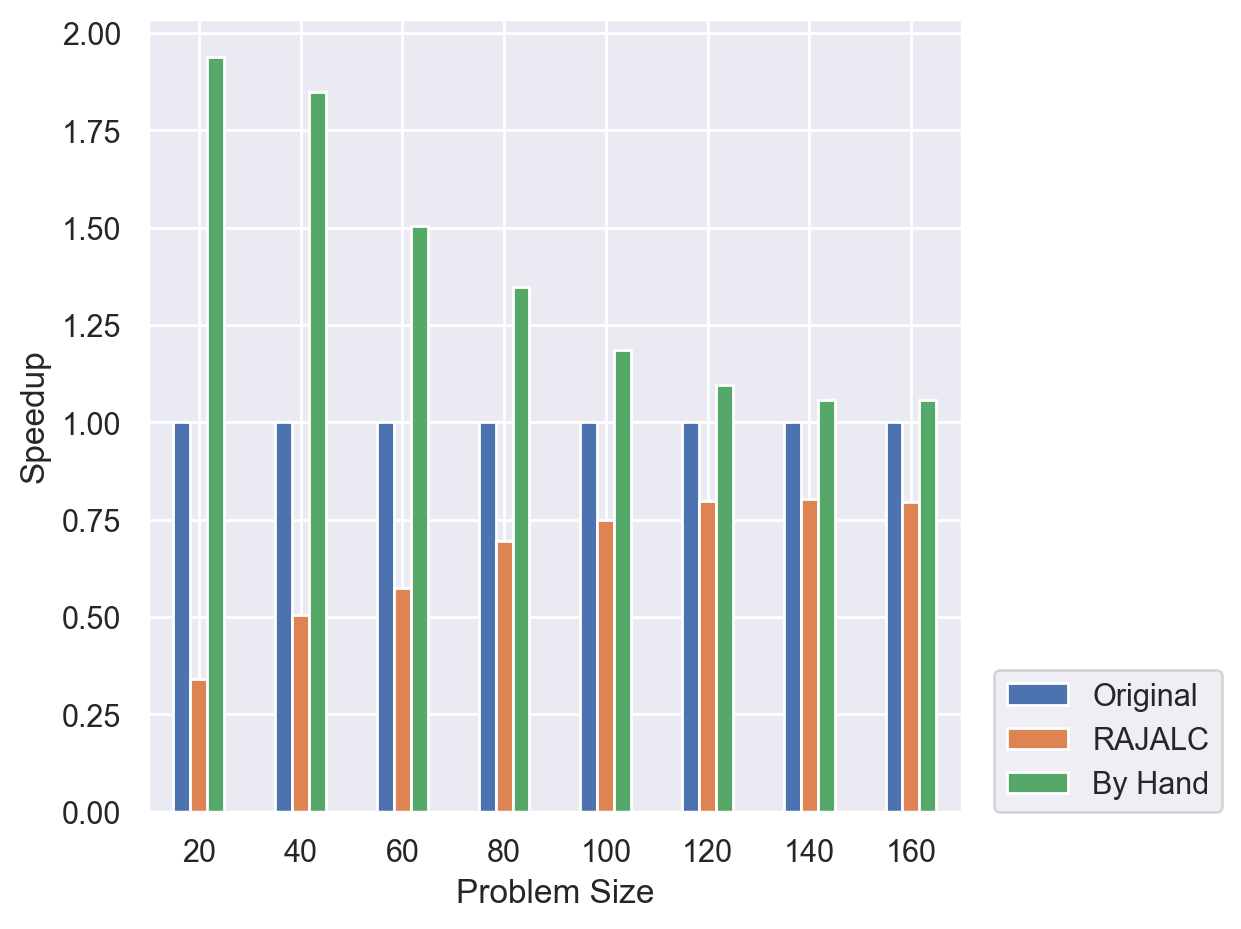
\includegraphics[width=\linewidth]{results/Lulesh/LuleshQuartzGcc8All/LuleshQuartzGcc8All.png}
\caption{LULESH Speedup on System Intel2 (higher is better).}\label{LULESHQuartz}
\end{figure}

\begin{figure}[t]
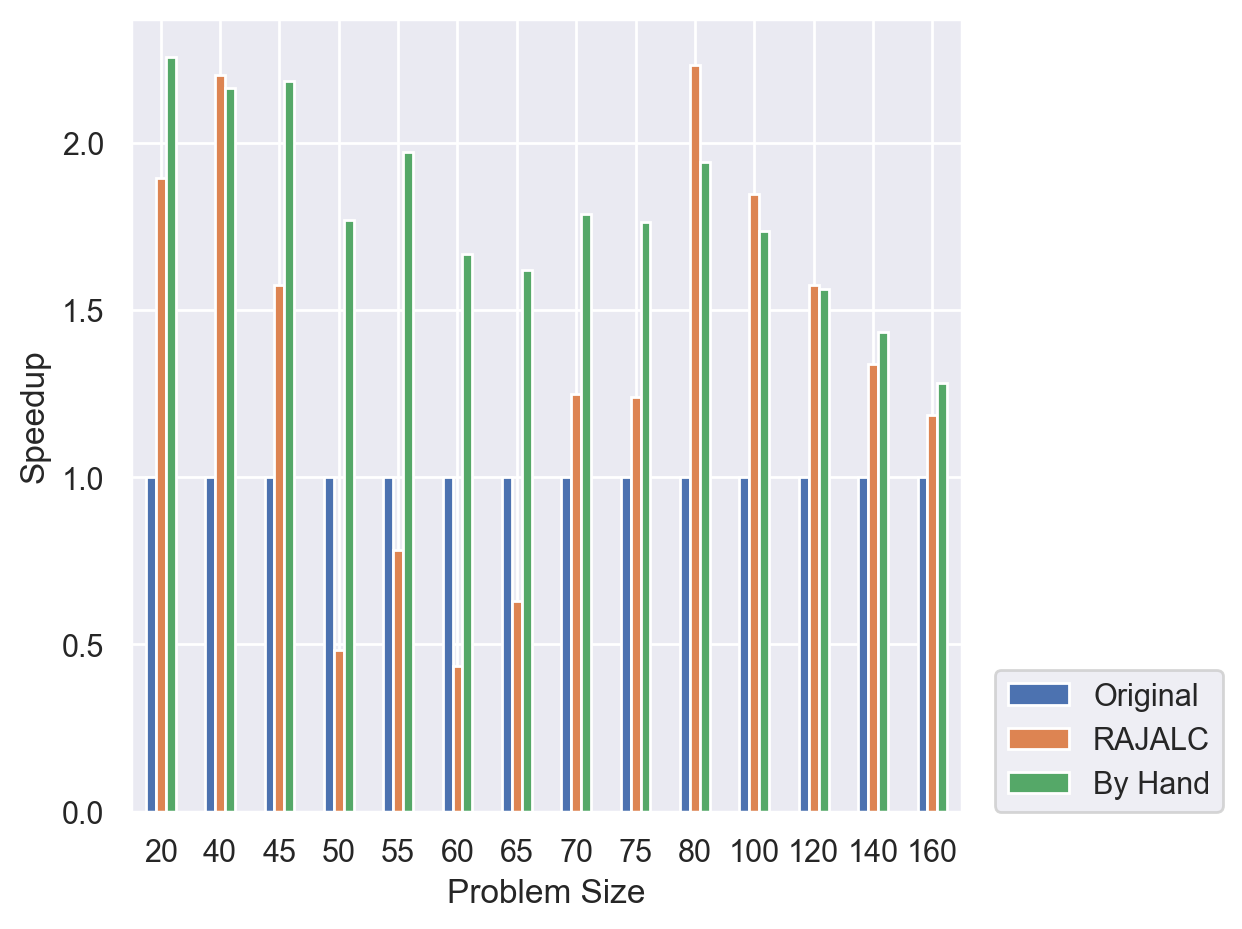
\includegraphics[width=\linewidth]{results/Lulesh/LuleshLassen/LuleshLassen.png}
\caption{LULESH Speedup on System Power9 (higher is better).}\label{LULESHLassen}
\end{figure}

Figures~\ref{LULESHRose},~\ref{LULESHQuartz}, and~\ref{LULESHLassen} show
the average speedup over three runs relative to Original for several problem
sizes. 
For the recommended problem sizes on Systems Intel1 and Intel2, RAJALC does
not see performance improvements, but By Hand does.
I expect improvement since the fused kernels are the same as \verb.ENERGY.
and \verb.PRESSURE. in RAJAPerf.
I examine the generated code with OptVis~\cite{devkota2020ccnav}, to uncover
two likely culprits.
First, although the RAJALC code includes inlining directives, some calls
within the fused kernel were not inlined. 
In the By Hand variant, the calls are always inlined by virtue of the code
being combined into a single lambda. 
Introducing multiple extra calls each iteration of the fused loop likely
contributes to the performance degradation with RAJALC\@
Second, the code for the kernels that were successfully inlined is dispersed
throughout the binary and contains more than twice as many basic blocks as
the By Hand variant. 
These extra jumps, often to completely different parts of the binary, also
likely reduce RAJALC performance. 
One method to reduce the first effect has been addressed by the authors 
in an OpenMP feature proposal. Modern compiler inlining directives are generally 
only suggestions to the compiler. A standardized, forced inlining directive would 
reduce the problem of extra calls within the kernel.
However, the implementation makes use of forced inlining directives, 
so future work will examine why these directives are not leading to the expected binary structure.

System Power9 exhibits much larger performance improvements, including at small
problem sizes. 
However, there is anomalous results for RAJALC for problem sizes around 60. 
I include additional problem sizes for System Power9 to contextualize this drop in performance. 
While not as significant, there is also volatility in the hand-implementation performance for these problem sizes.

\section{Related Work}

Several other approaches provide performance-portable loop optimization.
Inter-loop optimization has been studied for decades, but usually
within the context of domain-specific languages (DSLs).
This work aims to enable more general approaches within the performance portability library framework.

\subsection{Portable Intra-Loop Optimization}
RAJA~\cite{hornung2014RAJA}, OpenMP~\cite{OpenMPver5}, Kokkos~\cite{edwards2014kokkos},
and SYCL~\cite{SYCL2019} provide ways to parallelize and provide data locality
within individual loops.
For performance portability, Pennycook et al.~\cite{Pennycook2018} show an
example  that uses OpenMP to have a single source code with specializations
in pragmas to target different architectures.

%[Cuda has a way to schedule kernels in a queue so that data can be shared between
%those kernels?]  FIXME

Active libraries~\cite{VeldhuizenActive98} such as the 
Matrix Template Library~\cite{Siek:1999:SPM},
Blitz++~\cite{Veldhuizen2000},
and the Bernoulli compiler~\cite{ahmed2000framework,kotlyar1997relational} fuse some
computations using expression templates, but cannot fuse across statements.

\subsection{By Hand Inter-Loop Optimization}
Some work has experimented with overlapped tiling and other inter-loop
scheduling by hand.
Olschanowsky et al.~\cite{CathieSC14} showed that scheduling across loops and
reducing the temporary storage requirements led to problem size scaling and
significantly better performance in a CFD application.
Wahib and Maruyama~\cite{Wahib14} showed the importance of fusing kernel
computations for GPU execution.

Numerous approaches to scheduling across an outer ``time loop'' in a stencil
code have been investigated as early as 1998~\cite{Bassetti98,Wonnacott00}.  
The Cactus project~\cite{Ripeanu2001,Allen00cactus-gtoolkit} and 
Ding and He~\cite{Ding2001} demonstrated  overlapped tiling by expanding
ghost cells in stencil computations. 
Wonnacott and Strout~\cite{Wonnacott13} review many other approaches to
time tiling for PDE codes that do explicit stepping versus implicit stepping.

\subsection{DSLs Providing Inter-Loop Optimization}
A number of DSLs have been developed for specifying and
optimizing stencil computations.
The Pochoir work~\cite{Tang2011} embedded cache oblivious performance
optimizations to improve temporal locality in C++ code.
STELLA~\cite{Gysi2015}  and YASK~\cite{YASK2016} can specify and 
tune 3D finite difference stencil computations.
Rawat et al.~\cite{Rawat18} present a DSL called StencilGen for specifying
stencil computations.
They present algorithms that perform overlapped tiling within stencil
computations and heuristics for fusing between the computations for GPUs.
Their work demonstrates some possible performance benefits of scheduling
across stencil computations when targeting GPUs and CPUs. In contrast,
I present ways to enable and to control these optimizations across loops
in the context of a more general, parallel library, specifically RAJA\@.

LIFT~\cite{Hagedorn2018} is a data parallel, functional intermediate
representation that supports dense computations and stencil computations.
Once a computation written in a DSL is transformed to LIFT, pattern-based
transformation can implement optimizations such as overlapped tiling and
target many different architectures.
Krishnamoorthy et al.~\cite{krishnamoorthy2007effective} present an automated tiling
technique for stencil computations in which neighboring tiles perform
overlapping computations, which reduces communication and improves load
balance.

%[Image processing pipelines, which are also stencil applications.  
Embedded DSLs for image processing pipelines, such as
Halide~\cite{ragan-kelley2013halide} and
PolyMage~\cite{mullapudi2015polymage}, support orthogonally specifying and
scheduling stencil computations.
By exposing separate mechanisms for scheduling them, PolyMage supports
various scheduling, fusion, and tile size selection
algorithms~\cite{Mullapudi2016,Jangda2018,Adams2019}.
%BRANDON: Adding differentiation
However, using these embedded DSLs limits the expressible computation and requires prohibitive porting costs for large applications.
%Jangda and Bondhugula~\cite{Jangda2018} have developed heuristics for selecting tile sizes and
%fusing across image processing pipelines.
%[Compiler techniques that schedule across loops.  Requires code to be quite simple to be analyzed and 
%there have been a number of different heuristics for deciding when to fuse.]

%[DNNs optimizing across loops]
Several DSLs that specify deep learning neural network
architectures, including Halide extended for reverse mode automatic
differentiation~\cite{Li2018}, Tensor Comprehensions~\cite{Vasilache2018},
TVM~\cite{TVM2018} and Latte~\cite{TruongLatte2016} optimize across loops.
These DSLs have specific approaches to scheduling such as the Halide scheduling
algorithm for DNN~\cite{Yang2020}.
AutoTVM in TVM~\cite{Chen2019} learns how to schedule.
Frameworks like Delite~\cite{Sujeeth2014} for developing DSLs support 
cross-computation scheduling.

Although the DSL approach can better target a particular application domain,
this work schedules across loops within RAJA supports a broader class of
applications.
Further, I provide a different separation of concerns. RAJA handles
performance portability while the loop chain extension handles scheduling
across loops.
DSL approaches handle all of the scheduling and targeting of architectures,
which leads to not all architectures being covered in some cases.

\subsection{Traditional Compiler Approaches}

Loop optimizations are used in a wide variety of compilers.
Polyhedral optimizations have been incorporated into production compilers with Graphite~\cite{trifunovic2010graphite} and Polly~\cite{grosser2011polly}.
Both works have similar approaches, starting by extracting polyhedral representation from an intermediate representation. 
Graphite works on the GNU GIMPLE representation and Polly on LLVM-IR\@.
After extracting polyhedral representations, they perform a number of analyses and transformations and regenerate new, optimized code.
Both approaches are general-purpose, automatic approaches.

PLuTo~\cite{bondhugula2008pluto} is another example of an automatic optimizing compiler. 
While Graphite and Polly perform optimizations as they lower from code to executable, PLuTo is a source-to-source optimizer. 
While it focuses on balancing parallelism and locality through loop tiling, PLuTo also has the ability to fuse producer-consumer loops. 
PLuTo searches a large space of possible tilings, but it does so automatically, leaving minimal room for the developer to select their own transformations.

Other approaches like AlphaZ~\cite{yuki2012alphaz} and CHiLL~\cite{tiwari2009scalable} provide scripting languages that iteratively transform loops in the program. 
The programmer writes an additional file containing the transformations they want applied to loops in the program such as permute, tile, or unroll. 
While these approaches allow more flexibility in transformation and maintain the original structure of their code, they introduce an additional stage in the toolchain.
A similar drawback applies to embedded DSLs that use their own compilers, such as Tiramisu~\cite{baghdadi2019tiramisu}.




%%%%%
\subsection{Staging and Other Loop Chain Approaches}

The most related work to this submission is work that gathers representations of computations and other work that aims to specify and optimize loop chains.
Lightweight modular staging~\cite{LMS2012} presented an approach for gathering 
a representation of computation to enable scheduling across that implementation
in Scala.

Bertolacci et al.~\cite{Bertolacci2016,bertolacci2019using} propose extensions to
OpenMP pragmas to express and schedule loop chains.
The approach requires annotations about data accesses in the pragmas.
That work enables the specification of loop fusion and wavefront tiling. 

Luporini et al.~\cite{Luporini2019} has a similar goal of enabling the source
code that uses a library  (in this case Devito~\cite{Luporini2018}) to
schedule across loop computations that share data.
The loops in their case have indirect array accesses.
Thus grouping computations to improve data locality requires a run-time
inspection phase~\cite{Strout14IPDPS}.
Luporini et al.\ use various Python library interfaces to specify computations
using per-loop modularization and then a lazy-computation step that gathers
the loop descriptions and generates inspector-executor code for performing 
sparse tiling.
%% BRONIS: The following does not seem necessary; is not discussed
%% \begin{verbatim}
%%    with loop_chain(name, tile_size, fusion_scheme, ...):
%%        <some PyOP2 parallel loops>
%% \end{verbatim}

The key differences between their work and this one is that I leverage the view 
capability of RAJA to avoid needing to annotate how data is being accessed
in each loop.  
Instead, symbolic analysis collects that information.

\section{Conclusion}
Inter-loop optimizations have long been known to improve data locality and 
to reduce synchronization costs of computations with loops the share data
with producer-consumer relationships.
However, the required refactoring has remained a tedious manual process with 
significant impact on code maintainability.
We have presented a design that retains the loop-based modularization typical
of scientific codes while enabling the automated application of important
inter-loop optimizations.
RAJALC adds a loop chain construct and some API parameters to enable symbolic
analysis of data access patterns in the RAJA performance-portability C++
library. 
Importantly, their use entails minimal code changes. 




%\chapter{Data Transformations}\label{chap:FormatDecisions}

On today's high performance architectures, using the memory hierarchy effectively is a great challeng with a great reward.
When performance considerations --- architecture, memory hierarchy configuration, even input data characteristics --- are hard-coded into the application, improved memory performance comes at the cost of maintainability and portability.
This is especially relevant for schedule and data optimizations that are applied across loops, where the optimization obscures the underlying operation of the code.
To address this problem, performance portability libraries like RAJA, Kokkos, and YAKL provide abstractions for controlling how loops are scheduled/parallelized and how data is laid out initially. 
However, they do not support changing data layouts between loops without significant manual intervention.
This chapter's focus is on data layout transformations among canonical data layouts and the challenges inherent in enabling their high-level control within performance portability libraries, using RAJA as an example.
First, I introduce programming abstractions into the RAJA library to collect and apply data format transformations between kernels.
Then, I incorporate a built-in performance model for as-automated-as-desired transformation selection. 
Finally, to support key computations that benefit from these layout transformations, I extend RAJA's iteration space description to support loops with non-rectangular iteration spaces.
I also describe how the system could be used in a production code base to amortize modeling costs over multiple executions of the same program.
For computations with sufficiently large data sizes, this approach achieves similar performance to hand-implemented data layout optimizations with significantly fewer code changes across six key benchmark kernels.

\section{Introduction}

The gap between CPU speeds and memory latency recurs throughout computing history, prompting ever-more complex architectural solutions.
From the 384 byte ``B-store'' of the 1960 Ferranti Atlas~\cite{ferranti1960features} to the multi-level cache systems of today, memory hierarchy has endured as the solution.
The challenge is handed from the architect to the programmer, who must write programs that make use of this hierarchy efficiently.
There are two ways of doing this: changing the order in which data is accessed (loop schedules) and changing the order in which data is stored (data layouts).
The previous chapter focused on schedule transformations across multiple loops. 
This chapter focuses on runtime data layout transformations among canonical data layouts.

%Motivate the incorporation of data layout optimizations into PPLs
When optimizing code by hand, these transformations are onerous to implement.
The original, modularized implementation of a computation is obscured by the changes of implementing the transformation. 
When a code is meant to run on multiple systems or evolve to support new features, these optimizations can end up being more trouble than they are worth, the performance improvement offset by the increased maintenance and porting costs.

Performance portability libraries (PPLs) --- like RAJA~\cite{hornung2014RAJA}, Kokkos~\cite{edwards2014kokkos}, and YAKL~\cite{norman2022portable} --- partially address this problem.
By breaking the description of a computation into separable components, programmers can experiment with different schedules and layouts without obscuring the code's underlying operation.
However, control of the layout of data is limited to a global scope; data cannot be reorganized with different layouts throughout a computation.
Should they wish to change the data layout mid-program, they would have to use multiple arrays for the same data, ensuring that each maintain the correct contents.
The brave soul who chooses this option must still overcome yet another obstacle: selecting the right combination of formats.
Even a modest computation of two loops that use four 2D arrays has more than 200 combinations from which to choose, so trying all possible options quickly becomes infeasible. 

%Motivate the problems that arise from incorporation into PPLs
The transformations under consideration here, for example switching a 2D matrix from column- to row-major storage, are well known.
They have been incorporated as automatic transformations within distributed computing contexts as source-to-source research compilers for High Performance Fortran and Fortran D~\cite{bixby1994automatic,kennedy1995automatic,kennedy1998automatic}.
More recently, others have made efforts to incorporate user control of these transformations in domain-specific languages, such as DL~\cite{sung2012dl}, ExaSlang~\cite{kronawitter2018automatic} and Tiramisu~\cite{baghdadi2019tiramisu}.
These DSLs recognize the importance of giving the programmer control over how the program is optimized. %Significance of user indicating layout
However, both the automated and user-controlled approaches use compilers that are specialized, unstandardized, and in the case of HPF no longer existent.
For codes already written using PPLs, where using a standardized language and production-grade compiler is important, these approaches are not feasible.

%Focus on the challenges
Fortunately, performance portability libraries already contain data abstractions that can form the basis for supporting these transformations.
Still, there remain challenges.
The first is enabling programmer control of per-loop data layout without requiring it.
Addressing this requires an interface for specifying layouts that can be paired with automated selection.
Because necessary program analysis and modeling cannot be done at compile-time without modifying the compiler, it must be done at runtime and amortized or stored for use in subsequent executions.
This leads to the next challenge: the overhead of the analysis and performance modeling must be smaller than the improvements provided by the transformations.
Finally, important computations that benefit from layout changes, like correlation and covariance calculations, have iteration spaces where inner loop bounds depend on outer loop iterators, which is not supported by any of the three PPLs.  %Specific motivation of triangular iteration spaces

%Clear contributions
In this chapter, I present an approach that resolves these problems while balancing user control with automation, inspired by inspector-executor patterns often used in the realm of sparse computations~\cite{saltz1990run,saltz1991multiprocessors,Strout14IPDPS,strout2018sparse}.
I also present an implementation of this approach in the RAJA library.
To provide optional automated layout selection, a runtime performance model uses data access information gathered from symbolic evaluation (see Section~\ref{subsec:accesses}) and microbenchmarking results to solve an optimization problem based on previous approaches~\cite{bixby1994automatic}.
Rather than using an integer linear programming (ILP) formulation, I reduce runtime modeling time by using a nonlinear programming problem instead. 
This chapter makes the following contributions:
\begin{itemize}
\item An interface for combining user-specified layout choices with additional choices based on runtime modeling;
\item An optimization to the runtime benchmarking to increase the reuse of results;
\item An optimization to the model's optimization problem to reduce the number of variables by using a nonlinear formulation instead of a linear one; and 
\item Support for iteration spaces with parametric bounds, which includes triangular iteration spaces and are expanded in Chapter~\ref{chap:SparseRAJA} to support sparse iteration spaces. %connection of symbolic segments to sparse contribution
\end{itemize}

I begin with an overview of performance portability library data abstractions, and RAJA's in particular (Section 2).
Then, I expand the iteration space abstractions to support computations with relations between loop dimensions (Section 3).
Next, I introduce an interface for user-specified layout transformations between computations (Section 4).
This interface incorporates optional runtime modeling based on microbenchmarking to augment user choices without overriding them.
I build on existing automated approaches and make two key optimizations: one to reduce the number of model coefficients and one to reduce the number of model variables and constraints (Section 5).
Then, I sketch how the \FormatDecisions{} system might be used in a production code base (Scetion 6).
Finally, I evaluate the model's accuracy and performance, as well as the entire system's performance and productivity for six benchmark kernels and one application case study (Section 7).
I then review related work (Section 8), and conclude (Section 9).


\section{Background and Assumptions}

Each of the three PPLs has its own programming model and interface, yet the abstractions present in each have similarities.
Most relevant in this chapter are their respective multi-dimensional data abstractions.
This section reviews those abstractions and the assumptions made about codes that use \FormatDecisions{}.

\subsection{PPL Data Abstractions}

All three PPLs have a core multi-dimensional data abstraction around which the rest of the libraries are developed.
In Kokkos and RAJA, the abstraction is the \verb.View..
In YAKL, the abstraction is the \verb.Array..
The key feature shared by these types is that they decouple how the data is referenced from how it is stored.

How exactly the libraries achieve this decoupling differs in both name and method.
In YAKL, \verb.Array. objects have a ``style'' template parameter that indicate if the object should be C style (row-major) or Fortran style (column-major). 
The \verb.View. object in Kokkos also uses a template parameter to specify the mapping of indices to memory.
Kokkos has \verb.LayoutRight. for row-major storage, \verb.LayoutLeft. for column-major, and \verb.LayoutStride. for layouts with arbitrary dimensional strides.
In RAJA, the \verb.View. object is templated by a layout type as well, but the layout type itself does not specify the ordering of the dimensions. 
Instead, layout objects are instantiated at runtime with dimensional orderings and associated with the View when it is initialized.
This chapter is implemented in RAJA, which, combined with limitations of the symoblic evaluation capabilities presented in Chapter 2, lead to some assumptions about codes that use \FormatDecisions{}.

\subsection{Assumptions}
The \FormatDecisions{} system makes the following assumptions/requirements about the user program:
\begin{itemize}
\item Each array in the program can be modeled independently. \FormatDecisions{} sets up and solves one optimization problem per array and does not model interactions between arrays. For example, using two View objects sharing the same underlying sections of memory are prohibited.
\item Every data access is reachable and exercised by symbolic evaluation. All accesses must be incorporated into the performance model to produce accurate results, and these are identified using symbolic evaluation.
\item Modeled loops bodies do not use use iterators or data accesses as arguments to functions. This is to ensure compatibility with symbolic evaluation.
\item All arrays only use dense, hyper-rectangular data layouts, as \FormatDecisions{} only supports canonical layouts.
\item Modeled arrays have dimensionality less than or equal to six. This is the upper bound for dimensionality found in codes of interest, with six-dimensional data appearing in QCD codes.
\end{itemize}


\section{Transforming Data Layouts}

\begin{figure}
\begin{lstlisting}[caption={Changing data layouts for three Views in the \textsc{3mm} benchmark using \FormatDecisions.},
	label={FormatDecisions3MM}]
auto knl1 = make_kernel<KPOL>(segs1, [=](auto i0, auto i1, auto i2) {
	E(i0, i1) += A(i0, i2) * B(i2, i1);
});
auto knl2 = make_kernel<KPOL>(segs2, [=](auto i0, auto i1, auto i2) {
	F(i0, i1) += C(i0, i2) * D(i2, i1);
});
auto knl3 = make_kernel<KPOL>(segs3, [=](auto i0, auto i1, auto i2) {
	G(i0, i1) += E(i0, i2) * F(i2, i1);
});

auto decisions = format_decisions(ref_tuple(B,D,F), knl1, knl2, knl3);

decisions.set_format_for(B, {{1,0}}, knl1); // column-major
decisions.set_format_for(D, {{1,0}}, knl2); // column-major
decisions.set_format_for(F, {{0,1}}, knl2); // row-major
decisions.set_format_for(F, {{1,0}}, knl3); // column-major

// Generate and run the computations with format conversions
auto computation = decisions.generate();
computation();
\end{lstlisting}
\end{figure}

RAJA's existing support for changing data layouts is limited to the point of instantiation.
This work removes that barrier by providing a declarative data optimization system for specifying layout transformations between loops.
By combining user-guided layout specifications with optional automated support, \FormatDecisions{} gives the programmer more control over the optimization of their program.

\subsection{User-Guided Layout Transformations}

Consider the computation in Listing~\ref{SelectionExampleCode}.
Throughout the computation, the data is accessed in different orders.
For example, note the Views \verb.A., \verb.B., and \verb.D..
The order in which \verb.A. is accessed is different from \verb.D. because the argument order in their accesses are different.
In contrast, while \verb.B. and \verb.D. have the same argument order, their access orders are still different because they have different layouts.
Looking at the two references to \verb.F. in kernels two and three, we can see that even access order to the same data can change through a computation.
Because different formats are optimal for different kernels, this creates an opportunity for optimization. 

My approach, shown in action in Listing~\ref{FormatDecisions3MM}, introduces a single user-facing class, appropriately named \verb.FormatDecisions..
Rather than inserting code blocks to change a View's data layout between kernel executions, the user register choices for what format the data should have during different computations. 
Once the user has finished registering their choices, they can launch the supplementary model to identify additional optimizations or immediately generate the loop chain containing the computations and the conversions.

The user registers format decisions with two methods.
The first, \verb.set_format_for()., takes as arguments the View, the desired dimensional ordering, and the kernel or kernels for which the format should be used.
The second method, \verb.set_output_format()., takes a View and a dimensional ordering and ensures the View has that layout after the sequence of computations is done executing.
Lines 13 through 17 of Listing~\ref{FormatDecisions3MM} show four such registered choices.

While \FormatDecisions{} provide a supplementary decision model that can identify additional worthwhile layout changes, its use is not mandatory.
To ``fill-in'' the user's choices with those of the model, the programmer can use the \verb.model(). method.
Because this method uses the symbolic evaluation capabilities provided by RAJALC, it can only be used when the operations are supported for symbolic evaluation.
This means that the kernels cannot make indirect accesses (\verb.a(b(i)).), or call functions within the lambdas that use the iterators.

Regardless of whether the user has used the model or not, 
the complete computation with interspersed format conversions is generated using the \verb.generate(). method.

\subsection{Selecting Decision Semantics}

At first glance, it may seem that a single method for registering format choices would be sufficient. 
Simply provide the View, the computation, and the format to use during that computation.
However, it is often desirable to specify the format the data should be in at the end of the sequence of computations, especially when the sequence is run many times, for example as part of the time step in a simulation code.
A single registering function cannot provide this capability. 

Another important consideration is the semantics of the registered decisions. 
Should the user be registering format conversions or should they be registering the format with the assumption that any necessary conversion is made by the library?
I argue that it should be the latter.
First, registering formats is more declarative, as it does not dictate exactly how or when the data is converted to the desired format.
Second, registering conversions requires specification of both the input and output formats. 
Any conversion can be specified with two format registrations, but no number of conversion registrations can specify the same thing as a single format registration.

With these considerations in mind, I decided on two methods: \verb.set_format_for. and \verb.set_output_format..
When choosing this pair, the shorter \verb.set_format. was considered, but lacks the mnemonic match between the words of the method name and the parameter order. You \textbf{set} the View to \textbf{format} X \textbf{for} computation Y. 
Examples of these methods in use are shown in Listing~\ref{FormatDecisions3MM}.


\section{Automatic Layout Selection}

The \FormatDecisions{} class supports optional automated layout selection through the \verb.model(). method.
Broadly, the system constructs a search space of possible choices, estimates their costs based on a performance model, and selects the one with the lowest cost.
The problem of automatic layout selection has been formulated as an integer linear programming (ILP) problem by Bixby, Kennedy, and Kremer~\cite{bixby1994automatic}.
The system used within \FormatDecisions{} is similar to their formulation, but has several differences.
First, instead of using a static cost model, \FormatDecisions{} estimates costs using runtime microbenchmarking.
Second, it uses a modified heuristic for determining the candidate layouts to include in the model.
Finally, \FormatDecisions{} uses a nonlinear integer programming formulation, reducing the number of decision variables so much that even though the problem is no longer linear, the solve time is significantly reduced (see Section~\ref{sec:modelExperiments}).

This section begins with an overview of the layout selection problem and the prior formulation of Bixby, Kennedy, and Kremer.
It then details the modifications made in \FormatDecisions{}.
It concludes with six experiments that illustrate the effects of different parameters on model solve time, as well as the impact of the switch from a linear to nonlinear optimization problem.

\subsection{The Layout Selection Problem}

Layout selection is a numerical optimization problem.
It asks: Given an array and a series of $N$ loop nests accessing the data in $W$ different ways (e.g. \verb.A(i,j)., \verb.A(j,i)., \dots), what data layout should the array have during each loop nest to maximize performance?
Valid answers come as a list of $N+1$ layouts, one to use for each loop nest and one for the array to be in at the end.
For an isolated loop nest with only one kind of access to the array, the optimal answer is usually evident from a visual inspection of the code; the best layout is the one that matches the layout to the access order.
For example, in Listing~\ref{SelectionExampleCode}, \verb.T1. should be in row-major order, while \verb.B. should be in column-major order. 
However, when considering even two loop nests in sequence, the optimal choice is no longer statically evident.
This is because the benefit of using the optimal layout for a loop nest must be weighed against the cost of converting the data from one layout to another.
The challenge is further compounded by architectural differences that can affect both the cost of conversion and which layout will perform optimally.
The difficulty of this comparison lends itself to runtime automation.

Automating the layout selection problem, like many other decision problems, follows a two-step process: generate a set of valid solutions, then search the set for the best one.
Different problems operationalize these two steps in different ways, but a common approach is to model the decision problem as an integer linear programming (ILP) problem.
An ILP problem consists of a set of integer variables representing decision components, linear constraints over those variables representing the relationships between parts of the decision, and a linear objective function representing the costs of making different choices.
The solution to an ILP problem is a mapping of variables to values that satisfies the constraints and minimizes the objective function.
Once the solution to the ILP model has been identified, it can be mapped back to an optimal answer to the original decision problem.

Bixby, Kennedy, and Kremer (BKK) develop such a formulation for the layout selection problem~\cite{bixby1994automatic,kennedy1995automatic,kennedy1998automatic}.
They use a restricted type of ILP problem, known as a 0--1 ILP problem, that only uses binary variables.
Because the variables can only have the values 0 or 1, they can be conceptualized as on-off ``switches.''
Their formulation uses two types of variables: layout switches and remapping switches.
For each loop nest, or ``phase'', there is one layout switch for each possible layout.
Because an array has exactly one layout at a time, one and only one switch can be on for each phase.
Remapping switches represent the layout transformations that occur between phases of the program.
At each remapping point, there is one switch for each possible layout transformation.
As with layouts, only one remapping can occur at a time, so there will be one remapping switch turned on for each remapping point.
Remapping switches are also constrained to match the layout switches.
For example, if the row-major switch is turned on for both the first and second phase, the row-to-column-major remapping switch cannot be turned on.

Using this ILP model, valid solutions to the layout selection problem are represented by constraint-satisfying configurations of the switches.
For a $D$-dimensional array over $N$ loop nests, there are $D!*(N+1)$ such valid solutions, some better than others.
The objective function makes it possible to compare the quality of different solutions, ultimately leading to the best possible choice.
In the BKK formulation, the objective function is a sum of products, with one term for each switch.
Each layout variable is multiplied by a coefficient representing the estimated cost of using that layout for that phase.
Similarly, each remapping variable is multiplied by a coefficient representing the estimated cost of performing that layout transformation.
These cost estimates only contribute to the objective function value when their associated switches are turned on.
The configuration of switches that minimizes the objective function corresponds to a solution to the layout selection problem that should provide the best performance.

The accuracy of a solution relies on the accuracy of the model used to select it.
For the layout selection problem, the most important factor is the accuracy of the cost coefficients.
In the BKK formulation, the cost coefficients are calculated using static performance models based on pre-run training sets using vendor-specific communication libraries~\cite{kremer1996automatic}.
Thus, the quality of their layout selection system is entirely determined by the quality of this performance model.
Because the BKK performance model is static, each new machine requires a new and unique performance model be added to the system.
This limits the system's portability.

The model \FormatDecisions{} uses to solve the layout selection problem is a modified version of the BKK formulation.
There are three key differences.
First, the model is solved at runtime, rather than as part of a programming tool, using microbenchmarking results to inform the cost coefficients (Section~\ref{sec:microbenchmarking}).
Second, the model uses an alternative approach to selecting candidate data layouts (Section~\ref{sec:candidateSelection}).
Third, the model uses a nonlinear objective function (Section~\ref{sec:nonlinearFunc}).

\subsection{Runtime Solving and Microbenchmarking}\label{sec:microbenchmarking}

Where the BKK model is incorporated into a static, pre-compilation programming tool, \FormatDecisions{} solves the layout selection problem at runtime.
Because the model is solved at runtime, \FormatDecisions{} gains two sources of information not present in the BKK formulation.
First, \FormatDecisions{} has access to program parameters, like loop bounds and array sizes that are not available to the static BKK system.
Second, \FormatDecisions{} is able to more accurately estimate the costs of different data layouts by incorporating microbenchmarking results into the objective function.
These microbenchmarks are run as part of the program's execution, so they will be tuned to the architecture, system, and even the specific node on which the program runs.
While runtime solving can incorporate previously unavailable information, it comes with runtime overhead.
This runtime overhead must be outweighed by the performance improvement of the layout optimization, so the smaller the model, the better.
The second and third modifications to the BKK model are motivated by this need for a quick model, but first I turn to the runtime microbenchmarking.

\FormatDecisions{} uses runtime microbenchmarking to estimate the costs of using and converting among the candidate layouts. 
For different data accesses, a streaming copy with the same access pattern is timed at runtime.
The results of the microbenchmarking are incorporated into the model as the coefficients on the decision variables in the objective function.
The approach considers two types of costs: use costs and conversion costs.
Use costs represent the anticipated execution time associated with accesses to the data during the computation itself.
Conversion costs represent the anticipated execution time associated with converting from one format to another in between phases.
They use different approaches to determine their contributions to the objective function.

Use cost determination is access-based and proceeds through each kernel (phase) in the loop chain.
First, the kernel is symbolically evaluated and accesses to the View being modeled are isolated.
For each access, one term will be added for each candidate layout, estimating the cost of making that access with the candidate layout.
This estimate is the product of the microbenchmarking time and the number of loop iterations that make the access.
The microbenchmark is selected to match the traversal order of the access using that layout.

Collapsing the access, schedule, and candidate layout into the traversal order allows microbenchmark results to be reused for different variables. 
For example, for a constant schedule, the access \verb.A(i,j). in row-major layout has the same traversal order as the access \verb.A(j,i). in column-major layout.
Thus, their performance can be modeled with the same microbenchmark result. 
By reusing a single timing result for multiple decision variables, the overall time necessary to run the decision model is reduced.

Because the cost of conversion does not change based on the number of accesses to the data, these terms can be generated without reference to their surrounding computations.
Furthermore, they can be constructed while reusing the microbenchmarking results from the use cost estimation.
This is because a conversion from one layout to another can naturally be viewed as a kernel with two accesses: one access to data in the source layout and one to data in the destination layout.
Thus, the cost coefficient becomes the size of the array multiplied by the sum of the two access estimates.


\subsection{Candidate Layout Selection}\label{sec:candidateSelection}

The second modification refines how the model determines which layouts to include as candidates for selection.
The BKK formulation does not detail how their model makes this choice, but only discusses two-dimensional data, where there are only two possible orderings.
For higher-dimensional data, a simple option is to fully enumerate the possible layouts.
For two dimensional data, this gives two options; for three dimensional, six; for four, 24.
As the dimensionality increases, the number of layouts increases dramatically, and with it the modeling time.
Thus, an alternative formulation for selecting candidate layouts is needed.

Rather than using all $D!$ possible layouts, \FormatDecisions{} generates its set of candidate layouts using a seed set and a generating function.
The seed set is a small set of layouts that is expanded to a larger, final set of candidates using the generating function.
The seed set includes the original layout of the data, any layouts the user provides as part of registered decisions, and any layouts that \FormatDecisions{} calculates to match the access orders within the loop nests.
The generating function takes this set of seed layouts and generates the final set of candidates.
The generating function is user-configurable, but the default function is repeated rotation.
Rotating a layout means shifting each dimension to the right and moving the rightmost index to the leftmost position.
For example, consider the canonical three-dimensional layout $(0,1,2)$. 
In this layout, the first dimension has the largest stride, the second dimension has the middle stride, and the third dimension has a stride of one.
Rotating this layout onces produces the layout $(2,0,1)$, where the second dimension has the largest stride and the first dimension has the smallest.
Rotating again produces the layout $(1,2,0)$, where the last dimension has the last dimension has the largest stride and the middle dimension has the smallest.
Using this scheme, the number of candidate layouts is reduced from $O(D!)$ to $O(D)$, further reducing modeling time.

Repeated rotation was selected as the generating function for a confluence of reasons.
First, the generating function needs to generate options that are not present in the original set of options.
This excludes the identity transformation.
Second, different architectures perform better with different stride lengths.
While a CPU will do well with low-stride accesses, a GPU will perform better with large-stride accesses.
Because repeated rotation generates options where every dimension shows up once in each position, it is guaranteed to produce a wide range of stride lengths.
Finally, rotation is a staple, comprehensible transformation with transparent behavior.
This makes for easier reasoning about the model's decisions.
While it is possible that rotation will not surface the maximally performant layout for higher-dimensional data, the layout options it produce are a launching point for further experimentation.
Furthermore, user can supply an arbitrary generating function as long as it maps containers of layout permutations to containers of layout permutations.

\subsection{Nonlinear Objective Function}\label{sec:nonlinearFunc}

Minimizing solve time also led to the third key difference between the BKK formulation and the \FormatDecisions{} formulation: the use of a nonlinear objective function.
Execution time attributable to the ILP model comes from two sources: problem initialization (setup), and objective function minimization (solve).
The setup phase initializes the objects for the space of constrained decision variables and the objective function.
The more decision variables and constraints, the longer the setup phase.
The solve phase applies the objective function to the decision space and identifies the minimum point.
This too scales with the number of decision variables and constraints.
Using a nonlinear objective function can eliminate the majority of the decision variables in the problem.
While search time per decision variable increases with this scheme, the overall model time decreases significantly.

The nonlinear formulation reduces modeling time by completely eliminating remapping variables.
Recall that the BKK formulation uses two types of decision variables in its ILP model: layout variables and remapping variables.
Further, recall that the model constraints ensure the remapping variables between two phases are matched to the layout variables for those phases.
Given these constraints, the remapping variables are completely determined by the layout variables; 
if we know the values of the layout variables, we can always reconstruct the values of the remapping variables.
So then what is the purpose of the remapping variables? 
Simply, it is to incorporate the \textit{cost of remapping} into the linear objective function.
Because there are remapping variables for each pair of layouts, a model with $O(N)$ layout variables will need $O(N^2)$ remapping variables.
As a result, these faux variables end up dominating the entire model and bloat execution time.

Remapping variables are eliminated using a replacement scheme. 
Because their values are fully determined by the layout variables, remapping variables in the decision space and constraints containing them can be removed without incident.
This only leaves the terms containing remapping variables in the objective function.
These are replaced with equivalent terms that encode the removed constraints.
A remapping variable can only be switched on when the layout variables corresponding to its input and output are switched on.
This is a familiar operator: logical and --- or in the realm of boolean algebra, multiplication.
For example, all occurances of the remapping variable representing converting from row- to column-major between phases 1 and 2, $remap_{rowmjr \rightarrow colmjr}^{phase1 \rightarrow phase2}$, would be replaced by the product $layout_{rowmjr}^{phase1} * layout_{colmjr}^{phase2}$.
Thus, a replacement scheme can replace remapping variables in the objective function with products of layout variable.
This produces a nonlinear function, as it multiplies variables by other variables, but reduces the number of decision variables in the problem by a square factor.

\subsection{An Example Selection Problem}\label{exampleSelectionSection}
\begin{figure}
	\begin{lstlisting}[caption={Example loop chain. The selection problem targets the \texttt{A} array. Code is shown using standard C++ for loops rather than RAJA kernels for the reader's familiarity. All data is assumed to be initialized to $N \times N$ in row-major layout.},label=SelectionExampleCode]
		int N = 100;
		// data initialization omitted for brevity
	
	// knl1
	for (i = 0; i < N; i++) {
		for(j = 0; j < N; j++) {
			for(k = 0; k < N; k++) {
				T1(i,j) += A(i,k) * B(k,j);
			}
		}
	}
	//knl2
	for (i = 0; i < N; i++) {
		for(j = 0; j < N; j++) {
			for(k = 0; k < N; k++) {
				T2(i,j) += T1(i,k) * A(k,j);
			}
		}
	}
	//knl3
	for (i = 0; i < N; i++) {
		for(j = 0; j < N; j++) {
			for(k = 0; k < N; k++) {
				T3(i,j) += A(k,i) * T2(k,j);
			}
		}
	}
\end{lstlisting}
\end{figure}

An demonstration of the layout selection problem and the approach to solve it is instructive.
Consider the loop chain in Listing~\ref{SelectionExampleCode}, which calculates a series of matrix multiplications ($T1 = A * B$, $T2 = T1 * A$, and $T3 = A^\top * T2$).
The layout selection problem in this subsection will target the \verb.A. View, used in all three kernels in the example.
We construct the constrained decision space, then use microbenchmarking to construct the objective function.

The decision space construction starts with the selection of the candidate layout $L$.
For two-dimensional problems, the two candidates are row-major and column-major.
Within the system, these are represented as dimensional orderings --- $(0,1)$ and $(1,0)$ --- but for clarity's sake, we use their names here: $L=\{row,col\}$.

\paragraph{Decision Variables}
Once the candidate layouts have been identified, we can create the layout decision variables.
For each phase of the computation, including the input and ouput phases, there is one variable for each layout.
The subscript indicates the layout while the superscript indicates the phase. 
The 0 phase represents the input layout, while the $N+1$ phase represents the output layout.
For example, the $k_{col}^{3}$ variable indicates whether or not the array will use column-major order during the third phase (\verb.knl3.).
Thus, the full list of layout variables is: $[k_{row}^{0}, k_{col}^{0}, k_{row}^{1}, k_{col}^{1},k_{row}^{2}, k_{col}^{2},k_{row}^{3}, k_{col}^{3},k_{row}^{4}, k_{col}^{4}]$.
The $k_{row}^4$ and $k_{col}^4$ variables indicate what layout the data will be in after the loop chain has finished execution.

\paragraph{Constraints}
Now that the set of decision variables is created, the last step in creating the constrained decision space is the constraint expression. 
First, variables are constrained to be binary decision variables: either zero or one. 
For each decision variable $k$, we add the constraint $0 \leq k$ and $k \leq 1$.
Second, because an array can only have one layout at a time, we constrain the sum of the variables for each phase to be exactly one.
For example, to encode the fact that the array must be in either row- or column-major layout during the first kernel, we add the constraint $k_{row}^1 + k_{col}^1 = 1$.
In general, for each phase $i$, we add the constraint $\sum_{\ell \in L} k_\ell^{i} \ \ = 1$.
Finally, additional constraints are added based on decisions registered by the user.
For example, if the user specifies that the input and output formats should match, we would add $k_{row}^0 = k_{row}^4$ and  $k_{col}^0 = k_{col}^4$.
If the user specifies that the array should be in column-major for the second kernel, we would add $k_{col}^2 = 1$.

\paragraph{Objective Function}

\begin{figure}
	\begin{lstlisting}[caption={Microbenchmarking function for determining objective function cost coefficients. Code is shown for two-dimensional case for clarity. Note that the size of the data in the timed kernel does not change based on the size of the loops being modeled.},label=MicrobenchmarkingCode]
	size_t modelLayoutCost(Layout<2> l) {
		static std::map<Layout<2>, size_t> cacheMap;
		if (cacheMap[l] != 0) return cacheMap[l];

		int sideLength = sqrt(modelDataSize);
		View2D v1(new double[sideLength*sideLength], l);
		View2D v2(new double[sideLength*sideLength], l);

		// ... fill v1 and v2 with random data

		auto iterDim = RangeSegment(0,sideLength);
		auto iterationSpace = make_tuple(iterDim, iterDim);

		auto startTime = currentTime(); // millisecond resolution
		kernel<Pol2D>((iterSpace, [&](auto i, auto j) {
			v2(i,j) = v1(i,j);
		});
		auto stopTime = currentTime()
		auto elapsedTime = stopTime - startTime;

		cacheMap[l] = elapsedTime;
		return cacheMap[l];
	}
	
	\end{lstlisting}
\end{figure}
Constructing the objective function begins with estimating the cost of all accesses to the modeled View.
Starting with the first kernel, symbolic evaluation identifies one access, \verb.A(i,k)..
This access will contribute terms for the decision variables $k_{row}^1$ and $k_{col}^1$, one for each possible layout for \verb.A..
The term containing $k_{row}^1$ represents the estimated cost of using row-major storage for that access, while the term containing $k_{col}^1$ represents the estimated cost of using column-major storage.

Microbenchmarking happens here, running the timing function shown in Listing~\ref{MicrobenchmarkingCode} for row-major and column-major layouts.
Because this is the first access being considered, the function times and executes small streaming benchmarks using each layout. 
It stores the result in its cache map for later reuse.
For this example, assume the row-major layout return a time of 200 milliseconds, and the column-major layout returned a time of 400 milliseconds.
These results are fed into the performance model as part of the coefficients for terms of the objective function. 
For the cost of using row-major storage in the first loop (variable $k_{row}^1$), the microbenchmarking result is multiplied by the number of iterations in which the access appears, here 1000000 ($100*100*100$), and the decision variable.
This results in the objective function term $200 * 1000000 * k_{row}^1$. 
The same process is applied to represent the cost of using column-major storage, producing the objective function term $400 * 1000000 * k_{col}^1$.

In the next kernel, symbolic evaluation identifies another access: \verb.A(k,j)..
Note that with this access, the order of the iterators is reversed. 
As a result, the row-major timing result is used as the coefficient for the column-major layout, and vice versa.
The modeling result is always selected to match the data access pattern that the data would have for that layout.
For this access, the model will add the terms $200 * 1000000 * k_{col}^2$ and $400 * 1000000 * k_{row}^2$.

The third kernel proceeds similarly with the access \verb.A(k,i)..
The model will add the terms $200 * 1000000 * k_{col}^3$ and $400 * 1000000 * k_{row}^3$.

Next, the model adds terms to represent the cost of converting between layouts. 
For each pair of different layouts and consecutive kernels (including the input and output placeholders), one term is added representing the reads and writes required to convert layouts.
For example, to represent the cost of converting from column-major to row-major between kernels 2 and 3, the model will add $400 * 10000 * k_{col}^2 * k_{row}^3$ to represent the read of the column-major data and $200 * 10000 * k_{col}^2 * k_{row}^3$ to represent the write to the row-major data.
Both decision variables are part of the term to ensure the cost is only contributed when those layouts, and thus the conversion between them, are selected.

\paragraph{Solve}
Once the objective function is generated, it is applied to the space of layout choices, and the choice with the smallest score is identified.
This choice represents the layout transformations that the model predicts will lead to the fastest execution time.
For this example, the model will choose row-major for the first computation and column-major for the second and third.
Figure~\ref{fullExample} shows the full description of the decision space and objective function for this example problem.

\begin{figure}
\begin{subfigure}{\columnwidth}
\begin{gather*}
	\{ [k_{row}^{0}, k_{col}^{0}, k_{row}^{1}, k_{col}^{1},k_{row}^{2}, k_{col}^{2},k_{row}^{3}, k_{col}^{3},k_{row}^{4}, k_{col}^{4}] \ \ \vert \\
	\text{\texttt{/* binary variable constraints */}} \ \ 
	0 \leq k_{row}^0 \ \land \ k_{row}^0 \leq 1 \ \land \
	0 \leq k_{col}^0 \ \land \ k_{col}^0 \leq 1 \ \land \ \\
	0 \leq k_{row}^1 \ \land \ k_{row}^1 \leq 1 \ \land \
	0 \leq k_{col}^1 \ \land \ k_{col}^1 \leq 1 \ \land \ 
	0 \leq k_{row}^2 \ \land \ k_{row}^2 \leq 1 \ \land \ 
	0 \leq k_{col}^2 \ \land \ k_{col}^2 \leq 1 \ \land \ \\
	0 \leq k_{row}^3 \ \land \ k_{row}^3 \leq 1 \ \land \
	0 \leq k_{col}^3 \ \land \ k_{col}^3 \leq 1 \ \land \ 
	0 \leq k_{row}^4 \ \land \ k_{row}^4 \leq 1 \ \land \
	0 \leq k_{col}^4 \ \land \ k_{col}^4 \leq 1 \ \land \ \\
	\text{\texttt{/* single layout constraints */}} \ \ 
	k_{row}^0 + k_{col}^0 = 1 \ \land \ 
	k_{row}^1 + k_{col}^1 = 1 \ \land \ \\
	k_{row}^2 + k_{col}^2 = 1 \ \land \
	k_{row}^3 + k_{col}^3 = 1 \ \land \
	k_{row}^4 + k_{col}^4 = 1 \ \land \ \\
	\text{\texttt{/* user constraints */}} \\
	k_{row}^0 = 1 \ \land \ k_{row}^0 = k_{row}^4 \ \land \ k_{col}^0 = k_{col}^4
	\}
\end{gather*}
	\caption{Fully constrained decision space, including input/output matching and initialized type.}
\end{subfigure}

\begin{subfigure}{\columnwidth}
\begin{gather*}
	f(k_{row}^{0}, k_{col}^{0}, k_{row}^{1}, k_{col}^{1},k_{row}^{2}, k_{col}^{2},k_{row}^{3}, k_{col}^{3},k_{row}^{4}, k_{col}^{4}) = \\
	\text{\texttt{/* access in knl1 */}} \ \ 
	200 * 1000000 * k_{row}^1 \ + \ 
	400 * 1000000 * k_{col}^1 \ + \ \\
	\text{\texttt{/* access in knl2 */}} \ \
	400 * 1000000 * k_{row}^2 \ + \ 
	200 * 1000000 * k_{col}^2 \ + \ \\
	\text{\texttt{/* access in knl3 */}} \ \
	400 * 1000000 * k_{row}^3 \ + \ 
	200 * 1000000 * k_{col}^3 \ + \ \\
	\text{\texttt{/* conversions between phases */}} \\
	400 * 10000 * k_{row}^0 * k_{col}^1 \ + \ 200 * 10000 * k_{row}^0 * k_{col}^1 \ + \ 200 * 10000 * k_{col}^0 * k_{row}^1 \ + \ \\
	200 * 10000 * k_{col}^0 * k_{row}^1 \ + \ 400 * 10000 * k_{row}^1 * k_{col}^2 \ + \ 200 * 10000 * k_{row}^1 * k_{col}^2 \ + \ \\
	200 * 10000 * k_{col}^1 * k_{row}^2 \ + \ 200 * 10000 * k_{col}^1 * k_{row}^2 \ + \ 400 * 10000 * k_{row}^2 * k_{col}^3 \ + \ \\
	200 * 10000 * k_{row}^2 * k_{col}^3 \ + \ 200 * 10000 * k_{col}^2 * k_{row}^3 \ + \ 200 * 10000 * k_{col}^2 * k_{row}^3 \ + \ \\
	400 * 10000 * k_{row}^3 * k_{col}^4 \ + \ 200 * 10000 * k_{row}^3 * k_{col}^4 \ + \ \\
  200 * 10000 * k_{col}^3 * k_{row}^4 \ + \ 200 * 10000 * k_{col}^3 * k_{row}^4
\end{gather*}
	\caption{Fully expanded objective function, with timing results of 200 milliseconds for row-major layout and 400 milliseconds for column-major layout.}
\end{subfigure}

\caption{Full decision space and objective function for example selection problem in Section~\ref{exampleSelectionSection}. Loop nests are from Listing~\ref{SelectionExampleCode}.}\label{fullExample}
\end{figure}


\subsection{Six Parameters, Six Experiments}\label{sec:modelExperiments}

To illustrate the workings of the layout selection model, I evaluate its use for six synthetic programs that each vary one parameter: loop count, loop depth, memory footprint, access count, user constraint count, or data dimensionality.
Results are reported for two versions of the model.
The ``Linear Model'' panels use the BKK formulation of the optimization problem.
This means that it uses remapping variables, a linear objective function, and exhaustively enumerates the candidate layouts.
The ``Nonlinear Model'' panels use the optimized \FormatDecisions{} formulation.
This means that it does not use remapping variables, uses a nonlinear objective function, and uses the rotation heuristic for identifying candidate layouts.
For each experiment, I break the modeling time into the time spent modeling different access patterns, the time spent initializing the decision space and objective function, and the time spent identifying the optimal point within the decision space. 
Overall, data dimensionality, loop count, and user constraint count have the most impact on the modeling time.
Loop depth and memory footprint have no impact on modeling time, while access count has a small impact.

\begin{figure}
	\centering
	\includegraphics[width=0.7\columnwidth]{DataDimensionality.pdf}
	\caption{Changes in modeling time for data with different numbers of dimensions.}\label{DataDimensionality}
\end{figure}
The first parameter is the dimensionality of the data, varying in Figure~\ref{DataDimensionality} from two to six, the maximum dimensionality found in a production code (QCD).
The hypothesis is that the modeling time for the heuristic-driven model will increase linearly with the number of dimensions, because the number of variables is a linear function of the data's dimensionality.
This hypothesis is partially supported by the results.
Without reducing the set of candidate layout using the rotation heuristic, the execution reaches timeout before completing for four, five, and six dimensions.
For the version using the rotation heuristic, the solve time scales linearly with the dimensionality because the number of decision variables increases linearly with the dimensionality.
The cost estimation time scales faster than linearly. 
This may be caused by the increase in indexing calculation complexity as the dimensionality increases.
For example, each indexing expression in a 2D access calculates $i_1 + i_0 * N_1$, while a 4D access calculates $i_3 + i_2 * N_3 + i_1 * N_2 * N_3 + i_0 * N_1 * N_2 * N_3$.

\begin{figure}
	\centering
	\includegraphics[width=0.7\columnwidth]{LoopCount.pdf}
\caption{Changes in modeling time for different loop chain lengths.}\label{LoopCount}
\end{figure}
The next experiment, shown in Figure~\ref{LoopCount}, shows the modeling time for loop chains with between one and eight loop nests.
For this experiment, all loop nests are three-dimensional and make three accesses to two-dimensional arrays of $100\times100$ doubles. 
This size was selected to comfortably fit all data within cache.
No user constraints are added.
Because each new loop nest multiplies the number of possible paths by the number of candidates, the expected behavior is an exponential growth in solve time, which the results supports.
This experiment illustrates the execution time savings of eliminating the remapping variables from the model.
Using the linear model, because there are so many decision variables in the model, the majority of modeling time is spent in setup with as few as four loop nests (57\%).
Overall, the nonlinear model is between $1.29\times$ and $2.63\times$ faster than the linear model in this experiment.

\begin{figure}
	\centering
	\includegraphics[width=0.7\columnwidth]{NestDepth.pdf}
	\caption{(Lack of) Changes in modeling time for different depths of loop nests.}\label{NestDepth}
\end{figure}
The third experiment, shown in Figure~\ref{NestDepth}, shows the modeling time for loop chains where loop nest depth ranges from two to four.
Here, the loop chain contains three loop nests, and all other parameters are the same as the first experiment.
The hypothesis is that modeling time will remain constant across different nest depths.
This is because the performance model is array-oriented rather than loop-oriented, meaning it seeks to model the performance of each array access in the loop rather than the loop as a whole.
The results support this hypothesis, as Figure~\ref{NestDepth} shows no change to the modeling time across the three loop nest depths.

\begin{figure}
	\centering
	\includegraphics[width=0.7\columnwidth]{Footprint.pdf}
\caption{(Lack of) Changes in modeling time for different memory footprints.}\label{Footprint}
\end{figure}
The fourth experiment varies the size of the arrays accessed by the loop chain, shown in Figure~\ref{Footprint}.
The data sizes were selected to fill multiples of different levels of the evaluation machine's memory hierarchy, with a combination of half-filled, fully filled, or doubly-filled for each of L1, L2, and L3 cache.
These sizes were chosen because they exercise different parts of the memory hierarchy.
See Section~\ref{fillingSizesCalculation} for discussion of how these values are calculated.
Because the model only uses data sizes as coefficients in the model, the modeling times should remain the same as the memory footprint increases.
Aside from small fluctuations, the results in Figure~\ref{Footprint} support this hypothesis.

\begin{figure}
	\centering
	\includegraphics[width=0.7\columnwidth]{AccessCount.pdf}
	\caption{Changes in modeling time for different numbers of data accesses.}\label{AccessCount}
\end{figure}
Next is the number of accesses made to the data within the loop body.
Because modeling results are reused where possible, more accesses should not lead to more cost estimation time. 
However, it could lead to slightly higher solve times, as the objective function adds new terms for each access.
The results for this experiment, shown in Figure~\ref{AccessCount} are somewhat unexpected.
Cost estimation time scales with the access count.
This is likely due to cost of accessing the cache holding prior estimation results, as the cost estimation increase per additional access is much smaller than the cost of modeling a single access.

\begin{figure}
	\centering
	\includegraphics[width=0.7\columnwidth]{ConstraintCount.pdf}
	\caption{Changes in modeling time for different numbers of user-provided layout decisions.}\label{ConstraintCount}
\end{figure}

The final parameter is the number of layout decisions the user provides. 
Each additional layout decision adds one constraint, reducing the number of valid configurations. 
This should lead to a reduction in solving time, as there are fewer points to evaluate.
The results shown in Figure~\ref{ConstraintCount} support this hypothesis.

\section{Production System}

This section outlines a potential production system based on \FormatDecisions{} that uses representative training runs to entirely offload the overhead of running the decision model.
The production version would use a single feature not present in the prototype: decision I/O.
Specifically, to use the model results from a training run during a later production run, the system would need to be able to write out and read back in the model's layout decisions to persistent files.
This is not a completely trivial feature, but it is not a significant challenge, and I will return to it after outlining the system's function.

The production system would be run in one of two modes.
In the first mode, meant to be run with smaller but representative inputs, the system runs the decision model for each loop chain it encounters, writing the final, comprehensive layout choices to file.
In the second mode, meant to be used on the full production inputs, the system uses the layout choices produced by the training run.
Because the training run writes the full set of layout decisions for each loop chain, no modeling is necessary and the loop chains can be executed immediately.

Of course, it is not always possible to exercise all code paths with a single training run. 
For this circumstance, I propose a hybrid ``learning'' mode.
Meant to be run with full production inputs, it uses previous layout decision files when available and runs decision models for newly encountered loop chains.
Like the training mode, it writes the decisions to file, so that later runs can reuse the results.
With this scheme, newly encountered code paths will incur modeling costs for a single run, but not thereafter.

Returning to the problem of decision I/O, the key insight is that each \FormatDecisions{} object has a unique type in C++.
This is because its type contains the types of all the kernels within it, in the same way that the \verb.int. type is part of a \verb.std::vector<int>. type.
Two \FormatDecisions{} objects created from different kernels, or even from the same kernels in a different order, will have different types, much like a \verb.std::map<int, double>. object is a different type from a \verb.std::map<double, int>..
Thus, the decisions can be indexed by hashing the type of the \FormatDecisions{} object with which the decisions are associated.
Specifically, this can be achieved using C++ \verb.typeid. operator and the \verb.name. method on the resulting \verb.type_info. object.
This would ensure that decisions for a GPU execution are not used for a CPU execution, as the \FormatDecisions{} object types reflect the execution policy types of their constituent kernels.


\section{RAJAPerf Benchmark Evaluation}\label{fdEval}

This evaluation measures two features: model choice accuracy and system overhead.
Model choice accuracy refers to the accuracy of the runtime performance model by comparing the model decisions against those made by a heuristic-based hand-tuned variant.
This also includes the performance impacts of the model choosing different layouts.
System overhead refers to the runtime overhead from using the \FormatDecisions{} system.
I report two sources of overhead here: ILP overhead from setting up and solving the ILP problem and overhead from the layout selection abstractions.
Runtime microbenchmarking is included in the ILP overhead measurement.
Overall, for small problem sizes, ILP overhead was between $300\%$ and $700\%$ the performance improvement achieved by the transformation, meaning it was not able to amortize the cost.
For large problem sizes, ILP overhead was less than $25\%$.
Abstraction overhead was less than $30\%$ of the performance improvement across the board and negligible for large problem sizes.

\subsection{Experimental Design}

I evaluate the \FormatDecisions{} system using six benchmark kernels from the Polybench~\cite{pouchet2012polybench} benchmark suite: \textsc{2mm}, \textsc{3mm} \textsc{correlation}, \textsc{covariance}, \textsc{doitgen}, and \textsc{symm}.
\textsc{2mm} solves the matrix expression $A*B*C$ using two matrix multiplications. 
First, it computes $A*B$ and stores the results in a temporary array.
Then this temporary result is multiplied by $C$.
\textsc{3mm} solves a similar matrix expression $A*B*C*D$ using three matrix multiplications.
It computes $A*B$, then $C*D$, then multiplies the results.
\textsc{correlation} and \textsc{covariance}, as the names suggest, calculate the correlation and covariance matrix for the input data. 
\textsc{correlation} has four loop nests and \textsc{covariance} has three.
\textsc{doitgen} is a multiresolution analysis kernel while \textsc{symm} computes a symmetric matrix-multiplication.
These kernels, especially the matrix multiplication kernels, are ubiquitous computations.
They appear as building blocks across domains, found anywhere with linear algebra or statistics.

Each benchmark has four implemented variants. 
The baseline variant, ``RAJALC'', is implemented using the computation objects described in Chapter 2 and does not apply any layout transformations.
The second variant, ``Hand Tuned'', adds heuristic-based layout transformations \textit{without} using \FormatDecisions{}.
Data layouts are selected to match the access patterns of each computation, without attempting to estimate the tradeoff between conversion cost and performance improvement.
The third variant, ``Model Run'', uses the fully automatic \FormatDecisions{} system to select and apply layout transformations.
The only layout information provided to the model are the output formats for the data.
The fourth variant, ``Model Skipped'', uses the \FormatDecisions{} interface to fully specify the layout transformations given by the performance model, but uses the results of a previous model run.
Thus, this variant does not include overhead from running the performance model.
The difference between the execution times of the ``Hand Tuned'' and ``Model Skipped'' variants is the abstraction overhead, while the difference between the ``Model Skipped'' and ``Model Run'' variants is the ILP overhead.


\subsection{Evaluation Methodology: Machine Characteristics}
\label{fillingSizesCalculation}
I evaluate application performance on two machines: Lassen and Quartz.
All performance results are collected from single-node runs.
Lassen nodes use two 22-core 3.45GHz IBM Power9 CPUs.
However, a slow inter-socket connection is known to affect execution time consistency when the entire node is used by a single shared-memory program.
The conventional wisdom for Lassen is to treat each processor as its own node, so I run with 22 threads on a single processor.
Quartz nodes each have two 18-core 2.1GHz Intel Xeon E5--2695  CPUs.
Quartz runs in this chapter use a full 36 threads over both processors on the node.
Table~\ref{machineDetails} details the memory hierarchies for both machines.

\begin{table}[t]
	\centering
\begin{tabular}{|c|c|c|c|c|}
\hline
\textbf{Machine Name} & \textbf{L1 Cache} & \textbf{L2 Cache} & \textbf{L3 Cache} & \textbf{RAM} \\
\hline 
Lassen & 704KB & 16896KB & 120MB & 128GB \\ % https://hpc.llnl.gov/documentation/tutorials/using-lc-s-sierra-systems#POWER9
\hline
Quartz & 1152KB & 9216KB & 90MB & 128GB \\ 
\hline
\end{tabular}
\caption{Evaluation machine memory hierarchy characteristics. Cache sizes are given as total sizes for the the evaluation configuration.}\label{machineDetails}
\end{table}
%512*22 + 512*11 = 16896KB %lassen L2
%256*36 = 9216KB %quartz L2
%120MB %lassen L3
%45*2 = 90MB % quartz L3
%128GB % lassen RAM
%128GB % quartz RAM

For each benchmark, I run with six problem sizes on each machine. 
Each problem size half fills, fully fills, or doubly fills either L1 or L2 cache.
While I had attempted to run with sizes that fill L3 cache as well, preliminary executions timed out their node allocations before completing.
This is because the amount of computation scales faster than the amount of data ($N^3$ vs $N^2$).


The sizes for each benchmark are shown in Table~\ref{fillingSizes}.
To calculate these sizes, I use the array counts for the benchmark to construct a polynomial, the solution to which is the dimensional extent that fills a store of a particular size.
For example, the \textsc{covariance} benchmark has one 1D and two 2D arrays. 
To calculate the problem size that fills 704KB (Lassen L3 cache), which holds 60,000,000 doubles, we can construct the polynomial $2x^2 + x^1 = 60000000$.
The positive solution to this equation is the side length that will completely fill Lassen's L3 cache.
Because side lengths must be positive integers, I round down.

\begin{table}
	\centering
	\begin{tabular}{|c|c||c|c|c|c|c|c|}
		\hline
		\multicolumn{2}{|c|}{Benchmark} & SYMM & 2MM & 3MM & CORR & COV & DOITGEN \\ \hline
		\multicolumn{2}{|c|}{Dim Counts} & [0, 3] & [0, 5] & [0, 7] & [2, 2] & [1, 2] & [1, 1, 1] \\ \hline
	\hline
	Size Name & Data Size &   &   &   &   &   &   \\ \hline
	Lassen L1, .5x & 352KB & 242 & 187 & 158 & 296 & 296 & 55 \\ \hline
	Lassen L1, 1x & 704KB & 342 & 265 & 224 & 419 & 419 & 70 \\ \hline
	Lassen L1, 2x & 1408KB & 484 & 375 & 317 & 592 & 593 & 88 \\ \hline
	Lassen L2, .5x & 8448KB & 1186 & 919 & 776 & 1452 & 1453 & 161 \\ \hline
	Lassen L2, 1x & 16896KB & 1678 & 1299 & 1098 & 2054 & 2054 & 203 \\ \hline
	Lassen L2, 2x & 33792KB & 2373 & 1838 & 1553 & 2906 & 2906 & 256 \\ \hline
	Quartz L1, .5x & 576KB & 309 & 240 & 202 & 378 & 379 & 65 \\ \hline
	Quartz L1, 1x & 1152KB & 438 & 339 & 286 & 536 & 536 & 82 \\ \hline
	Quartz L1, 2x & 2304KB & 619 & 480 & 405 & 758 & 758 & 104 \\ \hline
	Quartz L2, .5x & 4608KB & 876 & 678 & 573 & 1072 & 1073 & 131 \\ \hline
	Quartz L2, 1x & 9216KB & 1239 & 960 & 811 & 1517 & 1517 & 166 \\ \hline
	Quartz L2, 2x & 18432KB & 1752 & 1357 & 1147 & 2146 & 2146 & 209 \\ \hline	
\end{tabular}	
\caption{Breakdown of benchmark data use and filling side lengths for different store sizes. The Data Dim Counts row indicates the number of arrays of different dimensionalities used in the benchmark. For example, [1, 2] means the benchmark uses a single 1D array and two 2D arrays. Filling side lengths are calculated by solving polynomials.}\label{fillingSizes}
\end{table}


\subsection{Results}
\begin{figure}
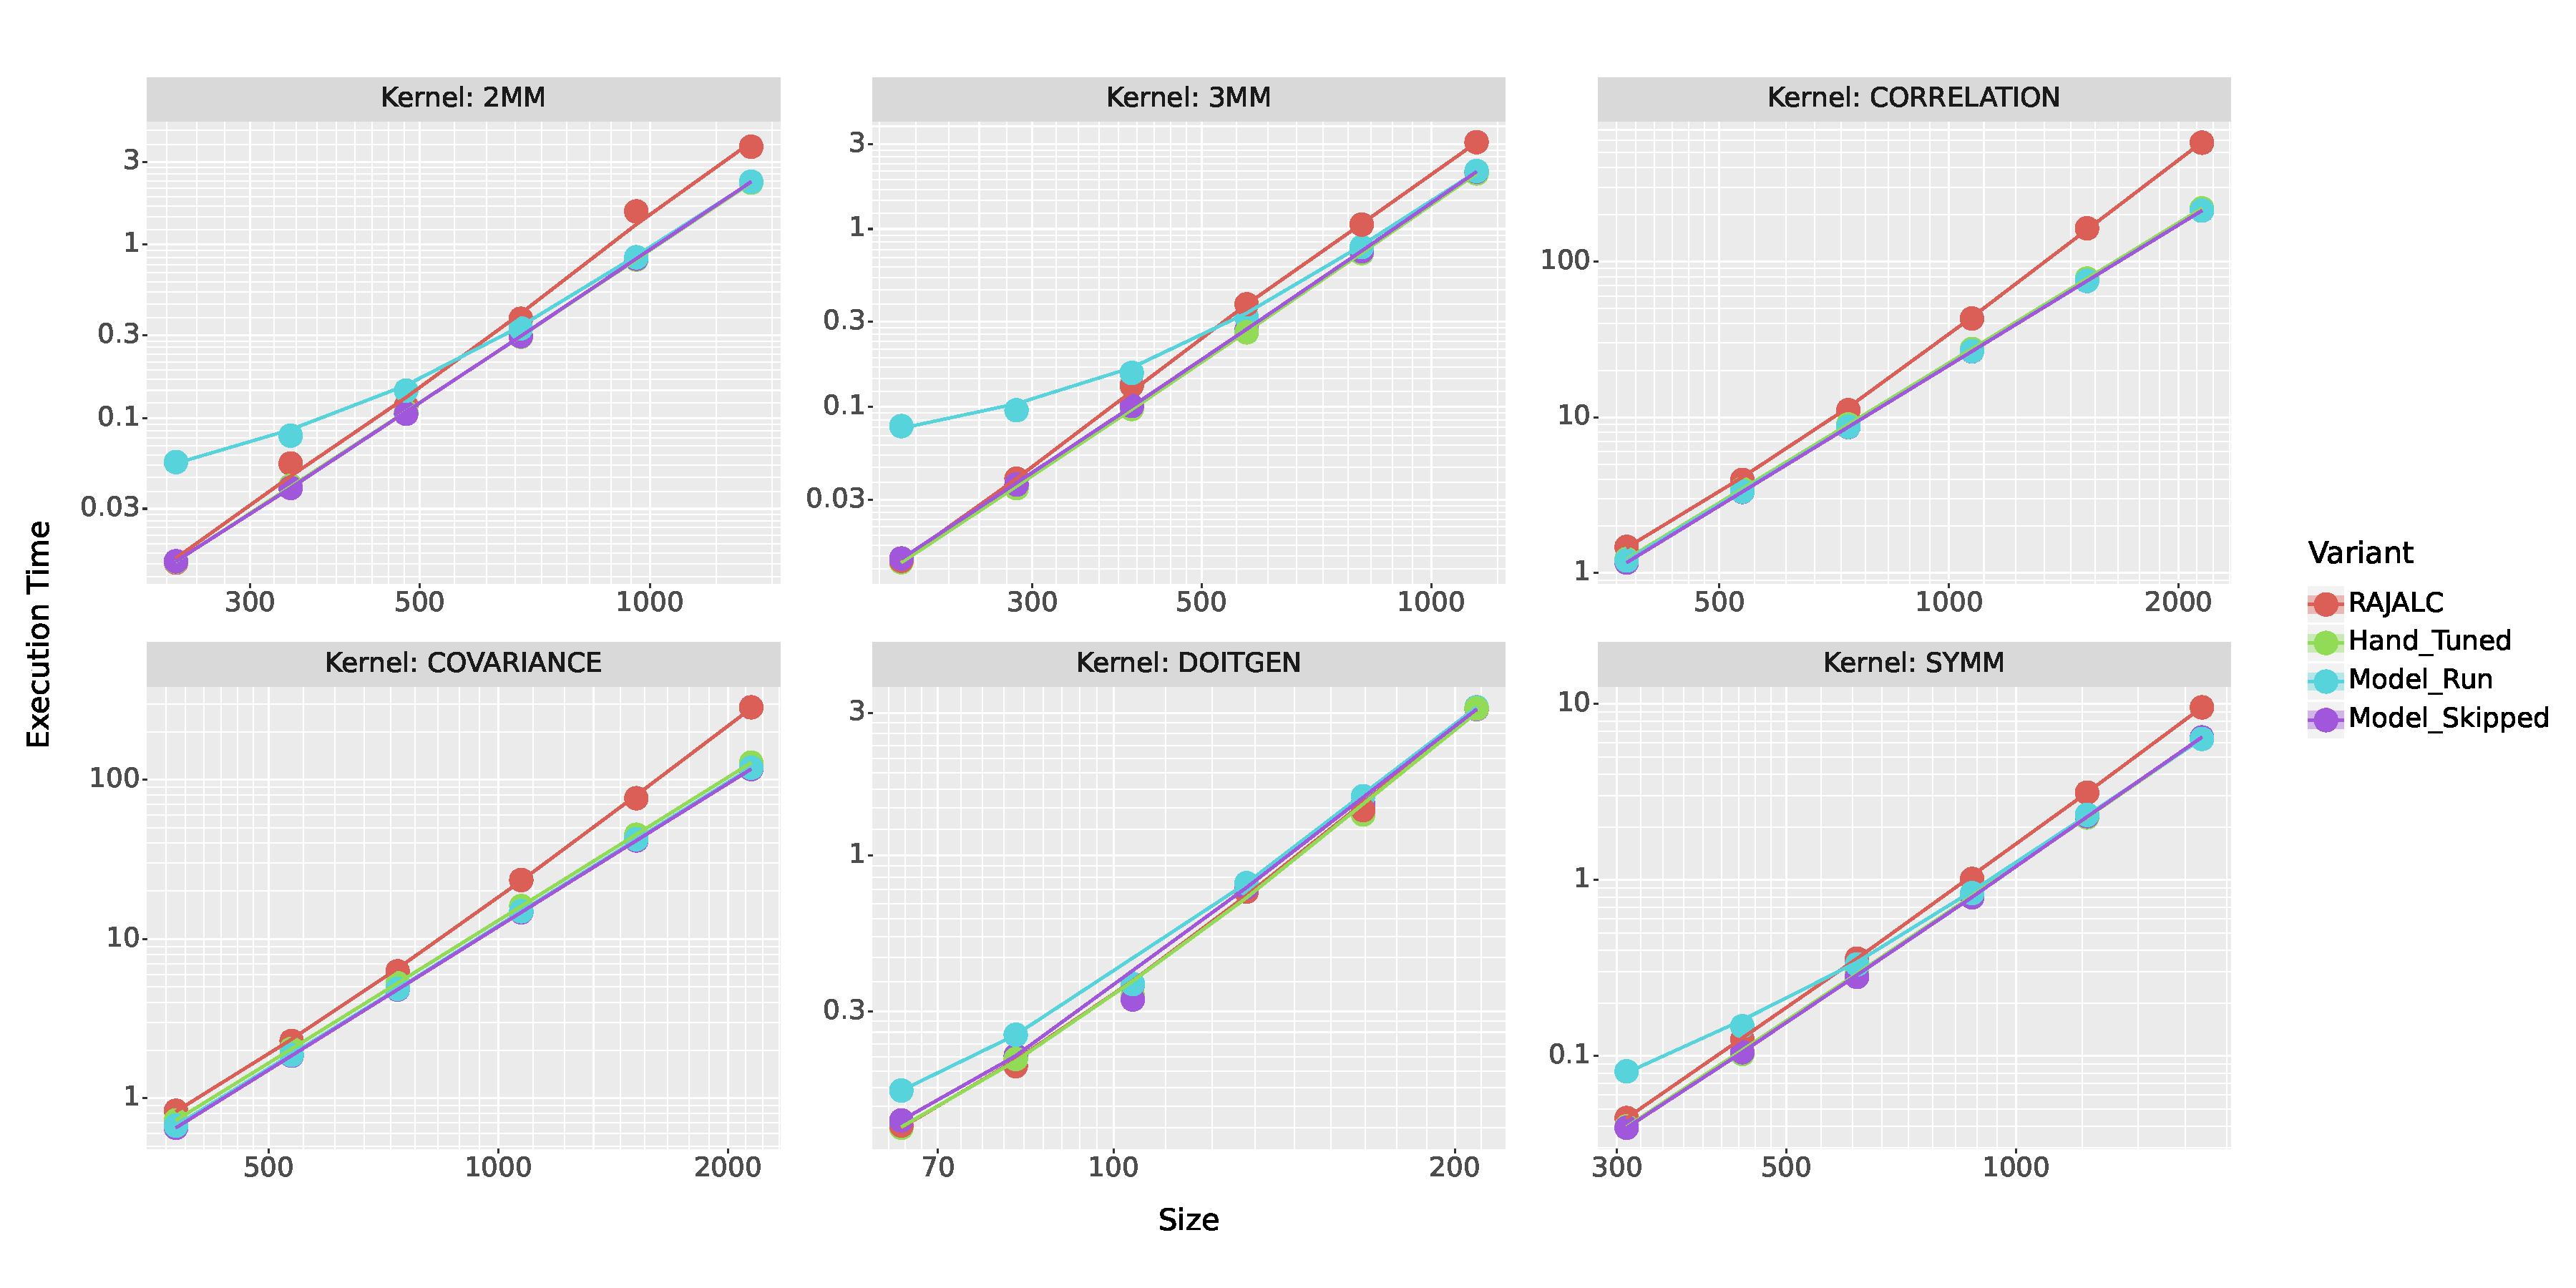
\includegraphics[width=\columnwidth]{quartz_speedups.pdf}
\caption{Execution times for evaluation on the Quartz system. Both axes are log-scale. Lower is better.}
\label{quartzSpeedups}
\end{figure}

\begin{figure}
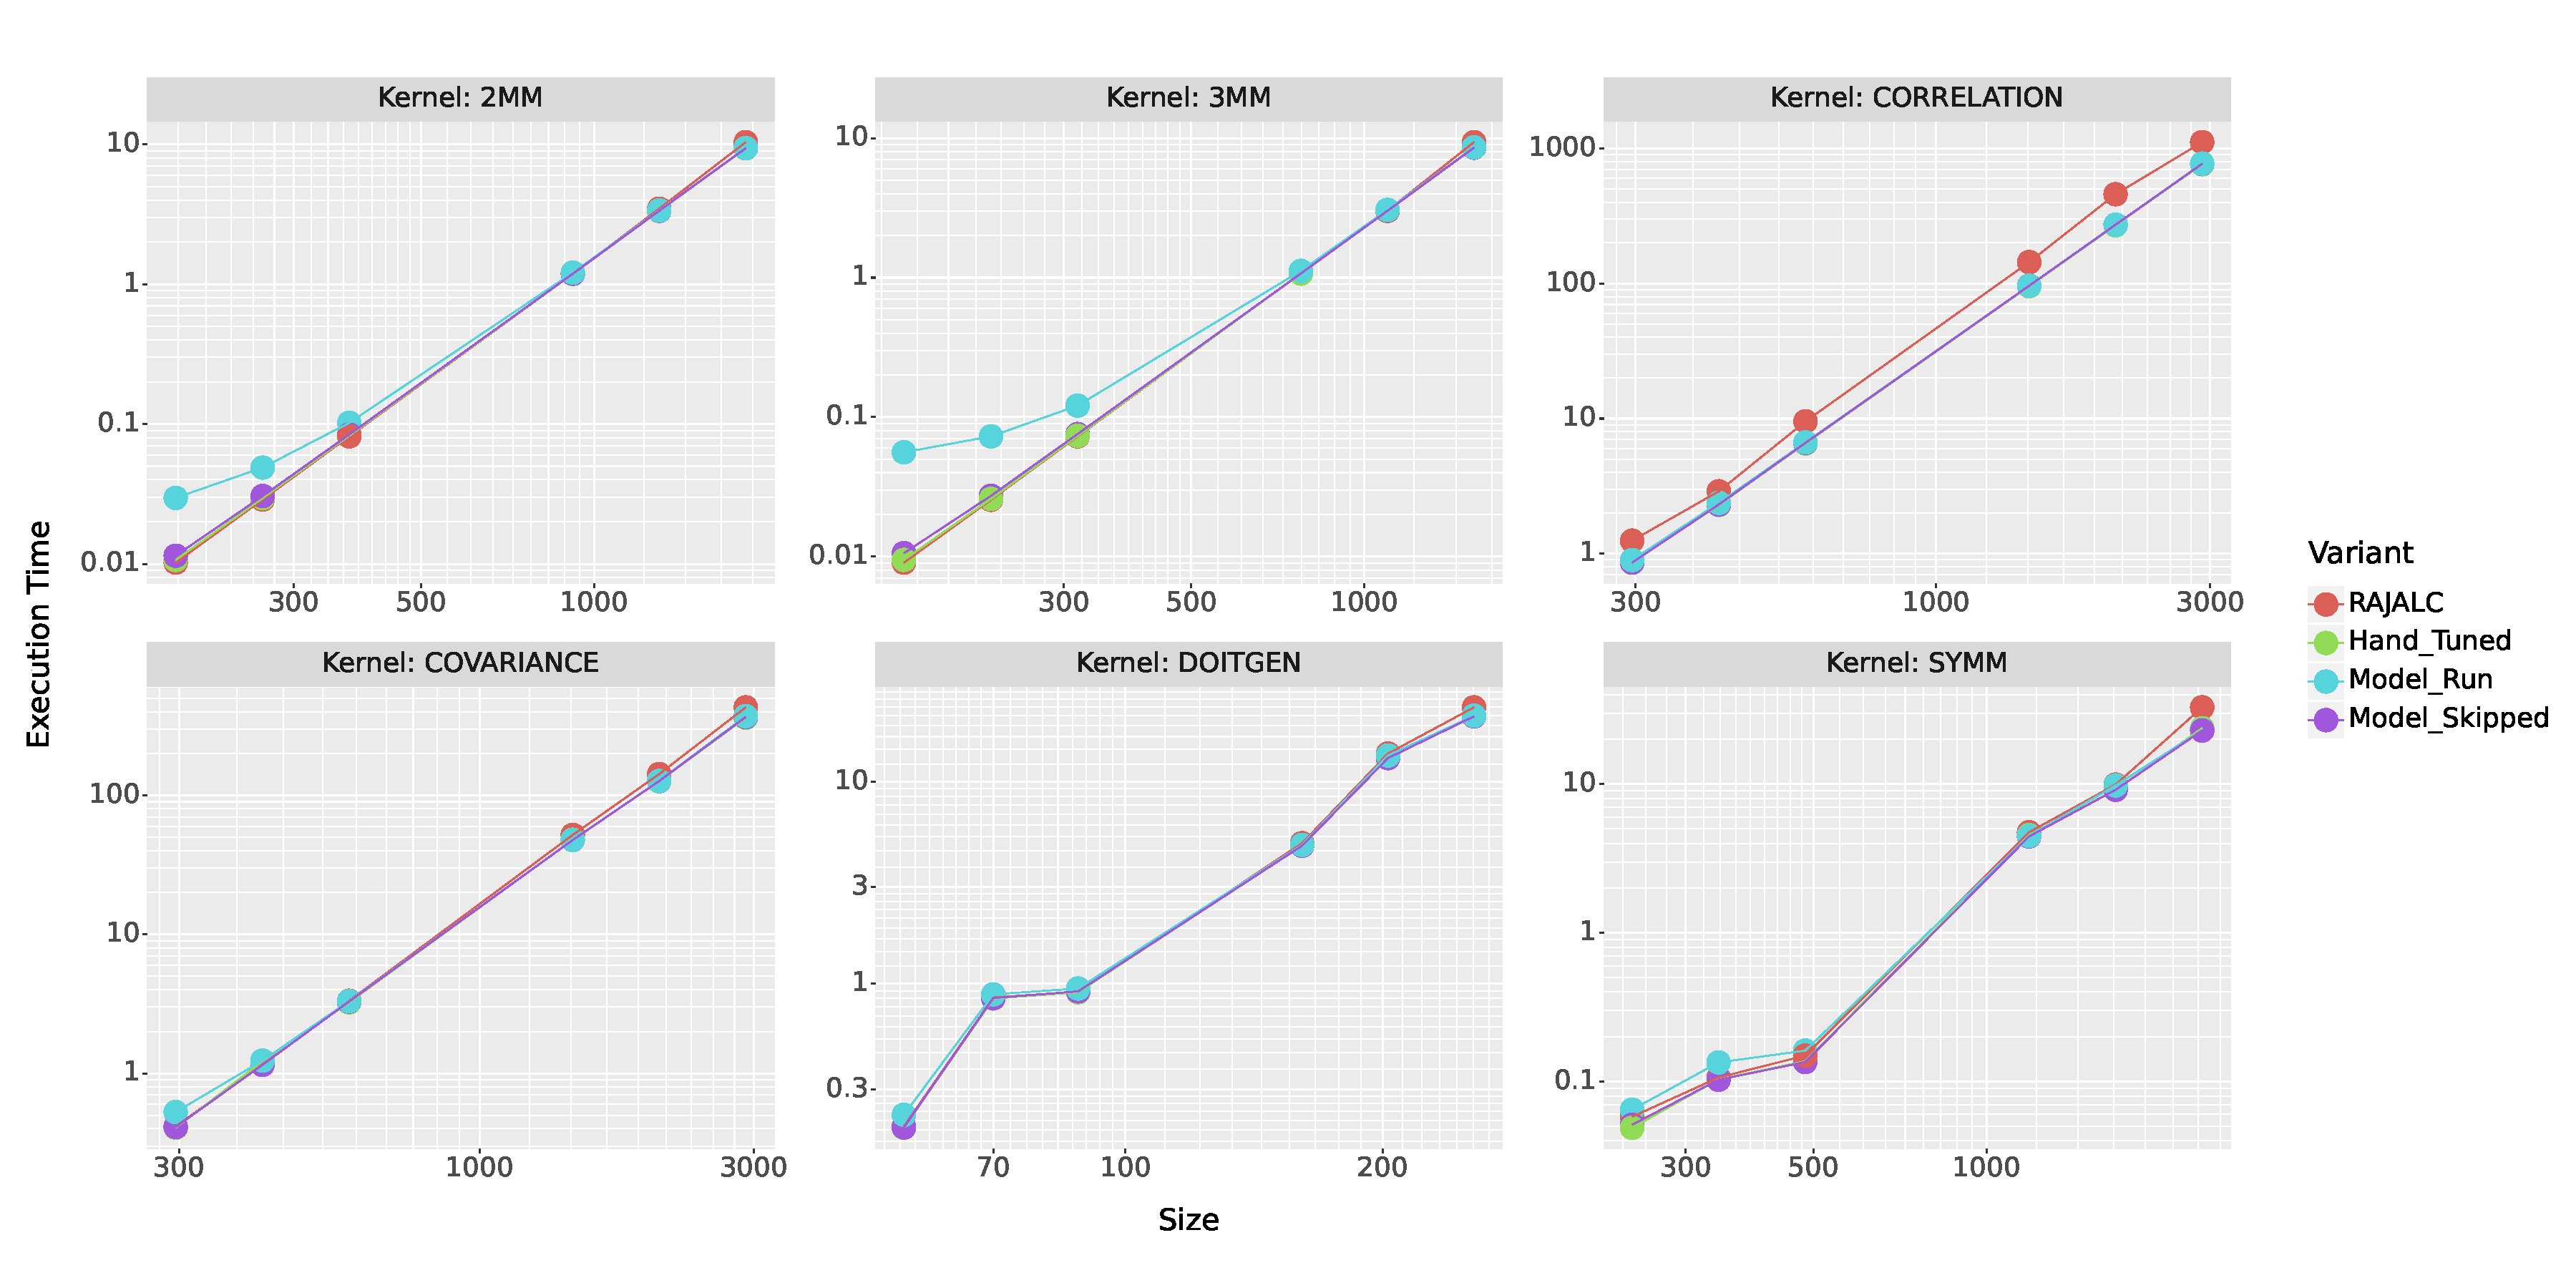
\includegraphics[width=\columnwidth]{lassen_speedups.pdf}
\caption{Execution times for evaluation on the Lassen system. Both axes are log-scale. Lower is better.}
\label{lassenSpeedups}
\end{figure}

Figure~\ref{quartzSpeedups} shows the execution times for the four variants on the Quartz system. 
For model accuracy, the only mismatches between the model-selected layout transformations and the hand-tuned heuristic selection were for the \textsc{3mm} variant.
For this benchmark, one of the target arrays, \verb.B., is only used in the first loop nest. 
Thus, the ``Hand Tuned'' variant converts to column-major before the first loop nest and back to row-major at the end of the entire loop chain.
The ILP model chooses to convert to column-major before the first loop nest, but immediately goes back to row-major instead of converting at the end of the loop chain.
Because the \verb.B. array is not used between the point the model chooses and the point the heuristic chooses, the difference does not affect the performance.

With regards to overhead, the ILP overhead (``Model Run'' vs ``Model Skipped'') was most significant for small problem sizes, especially for the \textsc{2mm}, \textsc{3mm}, \textsc{doitgen}, and \textsc{symm} kernels.
On average, for the smallest problem size, the modeling overhead was $387\%$ of the performance improvement achieved by the ``Hand Tuned'' variant.
This indicates that it is not possible to amortize the performance modeling cost for small problem sizes.
However, as the problem size increased, this overhead became less significant, as the solve time is constant no matter the problem size.
For the largest problem size, the modeling overhead was $23\%$ of the performance improvement of the ``Hand Tuned'' variant. 
The abstraction overhead (``Model Skipped'' vs ``Hand Tuned'') were negligible.
In some cases, especially for larger problem sizes, the ``Model Skipped'' variant slightly outperforms the ``Hand Tuned'' variant.
This is likely due to the highly templated nature of the code generated by the \FormatDecisions{} system allowing more aggressive compiler optimization.

Figure~\ref{lassenSpeedups} shows the results for the Lassen system.
The \textsc{3mm} benchmark produced the same mismatch between the heuristic choices and the model choices as on Quartz.
Otherwise, the model made the same choices as the heuristic-based approach.

Similar to the Quartz results, the ILP overhead was only significant for small problem sizes.
At the smallest size, the ILP overhead was $603\%$ of the performance improvement of the hand-tuned variant, meaning the ``Model Run'' variant took longer to execute that the baseline ``RAJALC'' variant.
The abstraction overhead was smaller, at $26\%$ of the performance improvement of the hand-tuned variant.
This means that it still saw performance improvement compared to the ``RAJALC'' variant, but less than the ``Hand Tuned'' variant.
For the largest problem size, the ILP overhead was much smaller, costing only $4.3\%$ of the hand-tuned performance improvement.
Like on Quartz, some benchmarks saw even greater performance improvements from using the \FormatDecisions{} abstraction without running the model.
On average, for the largest problem size, the ``Model Skipped'' variant saw $1.1\%$ improvement over the ``Hand Tuned'' variant.



\section{Parametric Iteration Spaces}

\begin{figure}
\begin{lstlisting}[caption={Comparison of C++ for-loop and RAJA \texttt{SymbolicSegment} representations of a loop nest with a triangular iteration space.},label=triangularComparison]
//C++ triangular for-loop
for(int i = 0; i < Ni; i++) {
	for(int j = i; j < Nj; j++) { // j starts at i
		... 
	}
}

//RAJA SymbolicSegments
auto iSeg = make_symbolic_segment(0, Ni);
auto jSeg = make_symbolic_segment(iSeg, Nj);
auto segments = make_tuple(iSeg, jSeg);
\end{lstlisting}
\end{figure}

\begin{figure}
\begin{subfigure}{0.4\columnwidth}
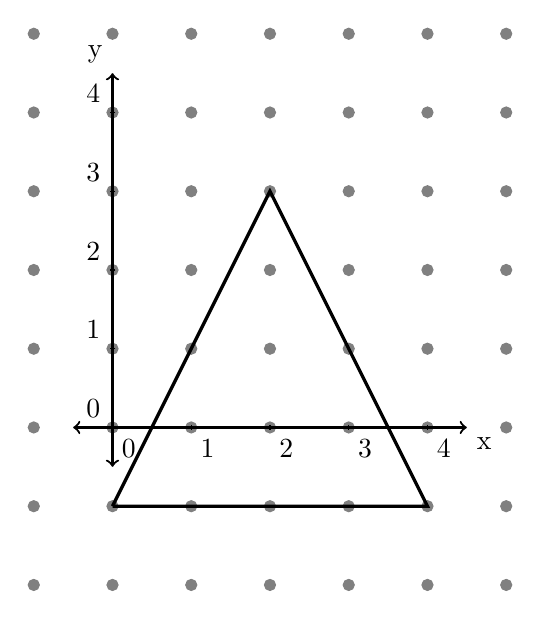
\begin{tikzpicture}
\foreach \x in {-1,0,1,2,3,4,5}
\foreach \i in {-2,-1,0,1,2,3,4,5}
	\filldraw [gray] (\x, \i) circle (2pt);
\draw[thick,<->] (-0.5,0) -- (4.5,0) node[anchor=north west] {x};
\draw[thick,<->] (0,-0.5) -- (0,4.5) node[anchor=south east] {y};
\foreach \x in {0,1,2,3,4}
	\draw (\x cm,1pt) -- (\x cm,-1pt) node[anchor=north west] {$\x$};
\foreach \i in {0,1,2,3,4}
	\draw (1pt,\i cm) -- (-1pt,\i cm) node[anchor=south east] {$\i$};
	
\draw [black, very thick] (0,-1) -- (2,3) -- (4,-1) -- (0,-1);
\end{tikzpicture}
\caption{Graphical depiction of iteration space with dependent $x$ dimension.}\label{triangularIterationSpace1}
\end{subfigure}
\hspace{0.05\columnwidth}
\begin{subfigure}{0.55\columnwidth}
\begin{subfigure}{\columnwidth}
\begin{align}
	-1 \leq &y < 4 \\
	(1 + y) * 0.5 \leq &x \leq (7 - y) * 0.5
\end{align}
\caption{Constraint description of iteration space from~\ref{triangularIterationSpace1}.}\label{constraintDescription1}
\end{subfigure}

\vspace{20pt}

\begin{subfigure}{\columnwidth}
\begin{lstlisting}[]
auto y_seg = make_symbolic_segment(-1,4);
auto x_seg = make_symbolic_segment_inclusive(
							(y_seg + 1) * 0.5, 
							(7 - y_seg) / 2);
auto segments = make_tuple(y_seg, x_seg);
\end{lstlisting}
\caption{Description of iteration space from~\ref{triangularIterationSpace1} using symbolic segments.}\label{symseg1}
\end{subfigure}
\end{subfigure}

\vspace{10pt}

\begin{subfigure}{0.4\columnwidth}
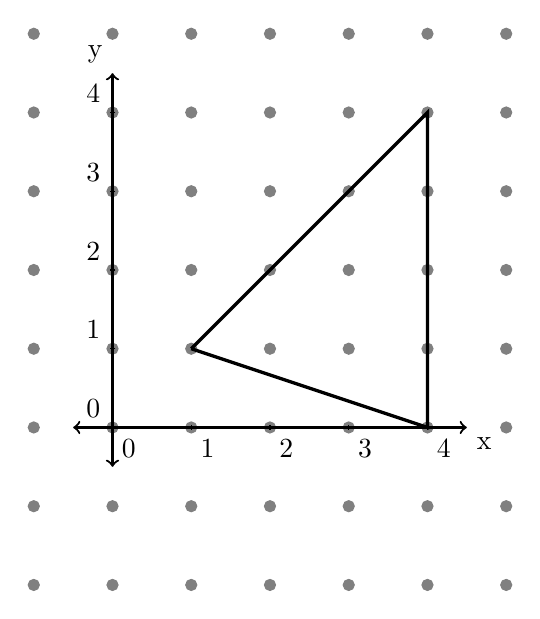
\begin{tikzpicture}
\foreach \x in {-1,0,1,2,3,4,5}
\foreach \y in {-2,-1,0,1,2,3,4,5}
	\filldraw [gray] (\x, \y) circle (2pt);
\draw[thick,<->] (-0.5,0) -- (4.5,0) node[anchor=north west] {x};
\draw[thick,<->] (0,-0.5) -- (0,4.5) node[anchor=south east] {y};
\foreach \x in {0,1,2,3,4}
	\draw (\x cm,1pt) -- (\x cm,-1pt) node[anchor=north west] {$\x$};
\foreach \y in {0,1,2,3,4}
	\draw (1pt,\y cm) -- (-1pt,\y cm) node[anchor=south east] {$\y$};
	
\draw [black, very thick] (1,1) -- (4,0) -- (4,4) -- (1,1);
\end{tikzpicture}
\caption{Graphical depiction of iteration space with dependent $y$ dimension.}\label{triangularIterationSpace2}
\end{subfigure}
\hspace{0.05\columnwidth}
\begin{subfigure}{0.55\columnwidth}
\begin{subfigure}{\columnwidth}
\begin{align}
	1 \leq &x < 5 \\
	(4/3 - x/3) \leq &y \leq x
\end{align}
\caption{Constraint description of iteration space from~\ref{triangularIterationSpace2}.}\label{constraintDescription2}
\end{subfigure}

\vspace{20pt}

\begin{subfigure}{\columnwidth}
\begin{lstlisting}[]
auto x_seg = make_symbolic_segment(1,5);
auto y_seg = make_symbolic_segment(
							(4 - x_seg) / 3, 
							x_seg + 1);
auto segments = make_tuple(x_seg, y_seg);
\end{lstlisting}
\caption{Description of iteration space from~\ref{triangularIterationSpace2} using symbolic segments.}\label{symseg2}
\end{subfigure}
\end{subfigure}
\caption{Two examples of representable triangular iteration spaces.}\label{goodTriangles}
\end{figure}



\begin{figure}
\begin{subfigure}{0.4\columnwidth}
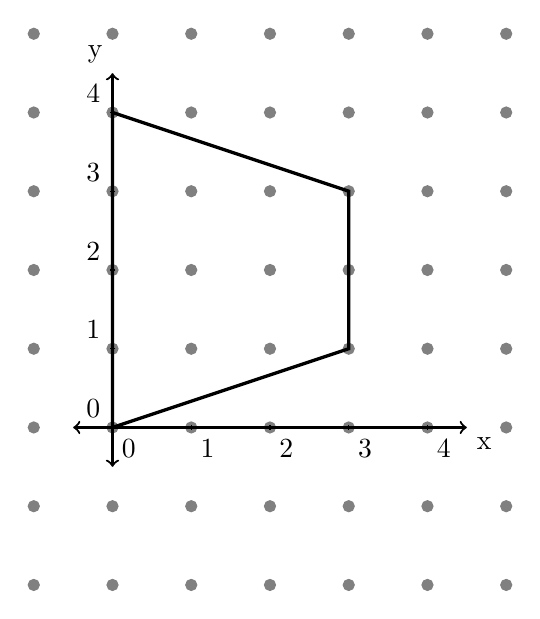
\begin{tikzpicture}
\foreach \x in {-1,0,1,2,3,4,5}
\foreach \y in {-2,-1,0,1,2,3,4,5}
	\filldraw [gray] (\x, \y) circle (2pt);
\draw[thick,<->] (-0.5,0) -- (4.5,0) node[anchor=north west] {x};
\draw[thick,<->] (0,-0.5) -- (0,4.5) node[anchor=south east] {y};
\foreach \x in {0,1,2,3,4}
	\draw (\x cm,1pt) -- (\x cm,-1pt) node[anchor=north west] {$\x$};
\foreach \y in {0,1,2,3,4}
	\draw (1pt,\y cm) -- (-1pt,\y cm) node[anchor=south east] {$\y$};
	
\draw [black, very thick] (0,0) -- (0,4) -- (3,3) -- (3,1) -- (0,0);
\end{tikzpicture}
\caption{Graphical depiction of quadrilateral iteration space with dependent $y$ dimension.}\label{trapezoidIterationSpace1}
\end{subfigure}
\hspace{0.05\columnwidth}
\begin{subfigure}{0.55\columnwidth}
\begin{subfigure}{\columnwidth}
\begin{align}
	0 \leq &x < 4 \\
	x / 3 \leq &y \leq 4 - (x / 3)
\end{align}
\caption{Constraint description of iteration space from~\ref{trapezoidIterationSpace1}}\label{trapezoidConstraint1}
\end{subfigure}

\vspace{20pt}

\begin{subfigure}{\columnwidth}
\begin{lstlisting}[]
auto x_seg = make_symbolic_segment(0,4);
auto y_seg = make_symbolic_segment_inclusive(
							x_seg / 3, 
							4 - (x_seg / 3));
auto segments = make_tuple(x_seg, y_seg);
\end{lstlisting}
\caption{Description of iteration space from~\ref{trapezoidIterationSpace1} using symbolic segments.}\label{trapseg1}
\end{subfigure}
\end{subfigure}
\caption{An example irregular quadrilateral iteration space that can be represented using symbolic segments.}\label{trapezoid1}
\end{figure}




While PPLs break the description of a computation into clear and separable parts, their approaches for representing iteration spaces are limited in expressivity.
The expressivity varies by PPL\@.
Kokkos is limited to iteration spaces composed of contiguous ranges.
YAKL additionally supports noncontiguous dimensions with constant strides.
RAJA is the most expressive, due to its \verb.ListSegment. abstraction, which supports iteration space dimensions with arbitrary lists of index values.
However, while any individual dimension can contain arbitrary values, they can only be composed into a multidimensional iteration space using the cartesian product (e.g., $[a, b, c] \times [1..3] = [(a,1), (a,2), (a,3), (b,1), \dots (c,3)]$).

Computations with iteration space dimensions that change throughout the computation, such as those with triangular iteration spaces, cannot be represented within this framework, nor can they be represented by previous works examining data layout selection~\cite{kennedy1998automatic}. 
Examples of these computations include LU decomposition, Cholesky factorization, and statistical calculations like covariance and correlation.
These are important computations in scientific computing.

To address this limitation in current PPLs and represent iteration spaces with relations between the dimensions, I introduce the \verb.SymbolicSegment. type to the RAJA library, which also forms the basis of the sparse iteration space description framework in Chapter~\ref{chap:SparseRAJA}. 
Unlike the \verb.RangeSegment., which requires integer values for its start, stop, and stride, the \verb.SymbolicSegment. supports bounds expressions that combine other segments with constant values. 
This process involves two elements.
First, the \verb.SymbolicSegment. objects maintain their current value through the execution of a kernel. 
Second, rather than returning a static value, the \verb.begin(). and \verb.end(). methods calculate the start and stop values dynamically based on the expressions used in their construction. 
When execution reaches the beginning of a loop, the symbolic bound expressions are evaluated and a standard \verb.RangeSegment. is instantiated for use in the loop.

Valid bound expressions in the definition of a \verb.SymbolicSegment. can contain numeric constants and previously defined symbolic segments, combined with the four basic arithmetic operators. 
By overloading the arithmetic operators to construct expression trees, the symbolic segments can delay evaluating the bounds of the dimension until that level of the loop nest is reached.
Further, it can \textit{re}-evaluate inner bounds expressions as the outer iterator values change.
This is a type of lazy evaluation of the loop bounds, resolving their dependences on outer dimensions at runtime.

This approach evaluates the bounds expressions only at the start of each nesting level, akin to the init-statement of a standard for-loop.
Once the bounds expressions are evaluated, the dimension is treated as a standard contiguous range, but maintains the iterator value within the \verb.SymbolicSegment. object itself.
This allows the value to be used in the evaluation of bounds expressions for deeper nesting levels.

When bounds expressions, like those in Figure~\ref{goodTriangles} contain division operations, evaluating them as integer expressions may lead to unexpected results. 
For example, as a lower bound, the expression \verb_1.5 - iSeg / 2_ resolves to $1$ when \verb.iSeg. has the value $0$. 
This is problematic, as $1$ is not greater than or equal to $1.5 - 0/2$.
The problem persists when expressions are rearranged to contain only integers; \verb.(3 - iSeg) / 2. suffers the same fate.
To address this issue, bounds are evaluated as floating point expressions then cast to integer values based on the bound type.
Lower bounds are cast to their ceiling, while upper bounds are cast to their floor.

Symbolic segments can readily express the triangular iteration spaces found in the computations mentioned above. 
Listing~\ref{triangularComparison} shows how a triangular iteration space written using a C++ nested for-loop is expressed using symbolic segments.
A regular segment has the same interface as \verb.RangeSegments.: \verb.iSeg = make_symbolic_segment(0,100);..
A segment that uses an outer loop index as its lower bound replaces it as expected: \verb.jSeg = make_symbolic_segment(iSeg, 100);..



\begin{figure}
	\begin{subfigure}{0.5\columnwidth}
	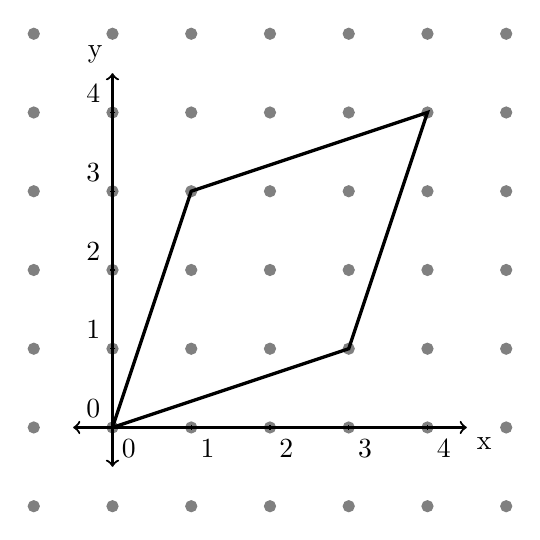
\begin{tikzpicture}
	\foreach \x in {-1,0,1,2,3,4,5}
	\foreach \y in {-1,0,1,2,3,4,5}
		\filldraw [gray] (\x, \y) circle (2pt);
	\draw[thick,<->] (-0.5,0) -- (4.5,0) node[anchor=north west] {x};
	\draw[thick,<->] (0,-0.5) -- (0,4.5) node[anchor=south east] {y};
	\foreach \x in {0,1,2,3,4}
		\draw (\x cm,1pt) -- (\x cm,-1pt) node[anchor=north west] {$\x$};
	\foreach \y in {0,1,2,3,4}
		\draw (1pt,\y cm) -- (-1pt,\y cm) node[anchor=south east] {$\y$};
		
	\draw [black, very thick] (0,0) -- (3,1) -- (4,4) -- (1,3) -- (0,0);
	\end{tikzpicture}
	\caption{Nonrepresentable skewed iteration space.}\label{skewedIterationSpace}
	\end{subfigure}
	\begin{subfigure}{0.5\columnwidth}
	\begin{subfigure}{\columnwidth}
	\begin{align}
		&y \geq x/3 \\
		&y \leq x/3 + 3 \\
		&x \geq y/3 \\
		&x \leq y/3 + 3
	\end{align}
	\caption{Constraint description of iteration space in~\ref{skewedIterationSpace}}\label{constraintDescription3}
	\end{subfigure}
	
	\begin{subfigure}{\columnwidth}
	\begin{lstlisting}
	for (int c1 = 0; c1 <= 4; c1 += 1) {
		for (int c2 = max(3 * c1 - 9, 
		                  (c1 + 2) / 3); 
				 c2 <= min(3 * c1, c1 / 3 + 3); 
				 c2 += 1) {
			...
		}
	}
	\end{lstlisting}
	\caption{C-style loop bounds generated using polyhedral code generator \href{https://compsys-tools.ens-lyon.fr/iscc/index.php}{ISCC}.}\label{farkasResult}
	\end{subfigure}
	
	\end{subfigure}
	\caption{An example of an irregular iteration space that cannot be represented using symbolic segments.}\label{badShapes}
	\end{figure}
\begin{comment}
Domain := [n] -> {
	T[x,y] : y >= x/3 and y <= (x+9) / 3 and x >= y/3 and x <= (y+9) / 3;
};
Schedule := [n] -> {
    T[i, j] -> [1, i, j];
};
codegen (Schedule * Domain);
\end{comment}


While symbolic segments enable the description of more loop nests than RAJA's base support, there are still iteration spaces that cannot be represented with them.
For example, iteration spaces resulting from loop skewing, often used to enable wavefront parallelism~\cite{wolf1991loop}, cannot be represented in this framework. 
Generally, iteration spaces that require the use of \verb.min. and \verb.max. in the description of the bounds are not supported by symbolic segments.
One approach to representing iteration spaces of this type is to describe the iteration space as a set of arbitrary linear constraints~\cite{verdoolaege2012polyhedral}.
This avoids the presence of \verb.min. and \verb.max. calls within the user's program.
However, this approach ultimately uses polyhedral scanning techniques~\cite{pouchet2007iterative,grosser2011polly, benabderrahmane2010polyhedral} to generate loop nests, which contain \verb.min. and \verb.max..
Adding a \verb.min. and \verb.max. expression to the \verb.SymbolicSegment. interface would technically enable the description of this class of polyhedra.
However, the user would either have to use an external tool to generate the expressions or calculate them by hand.
Because these polyhedra are rare in practice --- not appearing within the benchmarks evaluated here --- I chose to leave this feature as future work.

Symbolic segments enable PPLs to represent computations that were previously unavailable.
Using an interface based on the existing iteration space description in the RAJA library, they leverage a lazy evaluation strategy to calculate the bounds of a loop level only when needed.
One important pattern symbolic segments support is the triangular iteration space, found in three of the six evaluation benchmarks of Section~\ref{fdEval}.
Beyond enabling the decsription of triangular iteration spaces, symbolic segments form the basis upon which I develop support for representing sparse iteration spaces central to the next chapter.

\section{Related Work}

The approach used in this chapter to provide library-level abstractions for layout transformations is most closely related to the inspector-executor pattern found in sparse computations~\cite{strout2018sparse}.
In codes with sparse data, the distribution of the nonzero data heavily influences the most performant schedule and data alyout, but is not known until runtime.
The inspector-executor pattern resolves this dilemma by breaking a computation into an inspector phase, which analyzes the structure of the data, and an executor phase, which uses the results to select from different possible implementations.
This approach has traditionally been used to aid in parallelizing sparse codes~\cite{ujaldon1996parallelization,fu1996run,venkat2016automating}.
However, Venkat, Hall, and Strout have used it to select data transformations~\cite{venkat2015loop}.
\FormatDecisions' use of runtime performance modeling (inspecting) to determine the data layouts to use for the computation (executing) uses this pattern for a different class of computation.
It is also related to work on scheduling and data transformations, polyhedral compilation, and domain-specific languages.

\subsubsection{Schedule Transformations}
Early approaches to optimizing data locality use schedule transformations rather than data layout transformations. 
Work incorporated into the SUIF compiler uses interchange, reversal, skewing, and tiling~\cite{wolf1991data}, whereas Fortran source-to-source approaches also use loop fusion~\cite{mckinley1996improving}.
While schedule transformations avoid the overhead cost of layout conversion, their global nature can improve locality for one access while harming another.
Nevertheless, schedule transformations remain a popular approach to optimizing data locality and parallelism, 
especially through tiling techniques~\cite{bondhugula2008pluto,bertolacci2015parameterized,bondhugula2016diamond,bandishti2012tiling,unat2016tida}.

\subsubsection{Layout Transformation in HPF}
In the domain of data layout transformations, early work in High Performance Fortran (HPF) and D compilers~\cite{bixby1994automatic,kennedy1995automatic,kennedy1998automatic} provide foundations for a variety of later approaches.
Their framework follows a popular pattern: generate a space of possible choices, estimate the performance of different choices, and select an option using an ILP formulation. 
This chapter's ILP problem formulation is similar to theirs, although it does not use the data layout graph intermediate representation.
Furthermore, where their model for cost estimation focuses on communication costs in a distributed context, this approach models on-node performance costs of cache misses.

\subsubsection{Polyhedral Compilation}
The polyhedral model, traditionally used for schedule transformations, is commonly leveraged for data layout transformations as well.
With the rise of multicore chips, new strategies were needed to manage shared on-chip resources. 
Work by Lu et al.~\cite{lu2009data} and Zhang et al.~\cite{zhang2011optimizing} develop layout optimization schemes based on the polyhedral model and use a combination of strip-mining, permutation, and padding transformations.

\subsubsection{Heterogenous Computing}
Data layout transformation frameworks are also popular for heterogeneous programming systems, especially for stencil codes.
Sung, Stratton, and Hwu~\cite{sung2010data} use data layout transformations to relieve pressure on memory controllers in structured grid applications by spreading data out across the address space based on the indexing behavior of the application.
Henretty et al.~\cite{henretty2011data} develop a layout transformation and accompanying static analysis to address stream alignment conflicts for SIMD architectures.
Jaeger and Barthou~\cite{jaeger2012automatic} present a strategy for generating stencil codes with optimal data layouts using a multi-padding layout transformation.
Recognizing the need for specialized support for ever-changing chip structure, Majeti et al.~\cite{majeti2013compiler} develop a programmer (or autotuner) guided data transformation system.
Built into the Habenero-C compiler, the meta-data provided by the user guides the generation of architecture-specific SOA, AOS, and SOAOS data layouts.
Another approach by Kofler, Cosenza, and Fahringer~\cite{kofler2015automatic} convert AOS implementations to other data layouts for GPU applications automatically.  
With the exception of Majeti et al., these approaches do not provide an interface to the developer, and without exception are compiler-based approaches.
This approach presents an interface to the developer in the form of a library API, allowing user control and low-cost integration into existing workloads.

\subsubsection{Pragmas}
Although still in the realm of the compiler-based techniques, pragmas have been suggested as a solution to the problem of providing control over the transformations to the user.
Proposals to add such pragmas have been submitted to OpenMP~\cite{kruse2019design} and Clang~\cite{kruse2018user}.
Other work has implemented transformation pragmas into a source-to-source compiler~\cite{xu2014semi}. 

\subsubsection{Domain-Specific Languages}
Domain-specific language approaches are another avenue for presenting users with control of the data layout transformations to apply. 
Kronawitter et al.~\cite{kronawitter2018automatic} incorporate data layout specifications into the ExaSlang DSL.
Using a polyhedral framework, the Tiramisu DSL~\cite{baghdadi2019tiramisu} also enables data layout transformation specifications.
In constrast to these specialized approaches, the approach here seeks to support a wider class of computations without needing the additional machinery required to use DSLs. 


\section{Conclusion}

Effective use of the memory hierarchy is critical to application performance.
One way of doing this is by changing how data is stored within memory.
Yet, in performance portability libraries like RAJA and Kokkos, where one codebase is used for machines with different architectures, there are not yet tools for transforming the layout of data between parts of a computation. 
Thus, if a developer wants to introduce these optimizations, they are left in a time-consuming, error-prone situation --- further exacerbated by the potential for data layout transformations to not be worth the overhead.

\FormatDecisions{} remedies this situation by combining a declarative format specification interface with an automated decision model.
Integrated directly into the performance portability library RAJA, but possible in any library with computation objects and a data View-like abstraction, \FormatDecisions{} provides a flexible interface for quick exploration of data layout changes. 
Additionally, \FormatDecisions{} uses an ILP formulation to optionally identify other profitable transformations, \enquote{filling in} the user specification.

When evaluated against hand-implemented layout transformations on six benchmark kernels, \FormatDecisions{} provides comparable performance improvements for sufficiently large problem sizes with a fraction of the code changes.
Furthermore, subsequent modifications to the layout transformations, for example as part of porting a codebase to a new machine, are reduced to single-line changes. 
This improves maintainability and reduces the potential for introducing bugs.
Combined with the support for schedule transformations introduced in Chapter 2, performance portability library users can maintainably optimize a wide range of computations. 
The next chapter explores widening this range of supported computations even further.


%
\chapter{A Dense Survey of the Sparse Literature}


In this section, I aim to provide a somewhat detailed sketch of the development of sparse computation from modern computing's early beginnings to today.
Here, I focus on a series of related questions.
First, when and how did the notion of sparsity emerge?
Second, how did developments in computing technology (architecture, storage systems, etc.) and program representation (languages) influence thinking about sparse computation?
Third, where in the literature do we find the emergence of sparse \textit{tensors} in favor of sparse \textit{matrices}, and what factors caused this emergence? 
I do not purport to definitively answer these questions, only to offer hypotheses based on patterns that emerged in my excavation.
However, I believe that an historical engagement with the field offers deep insight into the open problems of today.

\subsection{The Notion of \enquote{Sparsity}}

Coming from an era when \enquote{computer} was a job title, the earliest work on computations on sparse data do not refer to them as such. 
This considerably increases the challenge of reasoning about the ideas of the time, but there remain important anchor points. 

Young's 1954 work developing iterative methods for elliptic PDEs~\cite{young1954iterative} presents the first elaboration of a sparsity property: nondescriptively called \textit{Property A}.
It places constraints on the distribution of nonzeros in a square matrix: An $N \times N$ matrix has \textit{Property A} if there exist a 2-partition $S,T$ of the first $N$ integers such that if matrix entry $a_{i,j} \neq 0$, then $i=j$ or $i \in S \land j \in T$ or $i \in T \land j \in S$. 
Examples are shown in Figure~\ref{propAExamples}.
While Young does not discuss using the property to guide implementation, he does give estimated UNIVAC calculation times for different problem sizes.
\begin{figure}[h]
\begin{lstlisting}[caption={Entry pattern for $N=6,T=\{0,5\},S=\{1,2,3,4\}$ maximal \textit{Property A} matrix}]
  * * * * * 0
  * * 0 0 0 *
  * 0 * 0 0 *
  * 0 0 * 0 *
  * 0 0 0 * *
  0 * * * * *
\end{lstlisting}
\begin{lstlisting}[caption={Entry pattern for one $N=2,T=\{0\},S=\{1\}$ \textit{Property A} matrix},label={propAnonSym}]
  0 0
  * 0
\end{lstlisting}
\caption{Example nonzero patterns of \textit{Property A}. }
\label{propAExamples}
\end{figure}

Like Young, Wilf~\cite{wilf1960almost} elaborates a matrix property that constrains the distribution of entries. 
His \enquote{almost diagonal} matrices differ from a diagonal matrix by a matrix of rank one. 
Formally, a matrix $A$ is almost diagonal if there exists a diagonal matrix $D$ and vectors $x$ and $y$ such that $A = D + xy^t$. 
Like Property A, almost-diagonality suggests a specialized a sparse representation.
$A$ is stored as three vectors, one for each of $D$, $x$, and $y$.
Then, any access $A(i,j)$ could calculate its value on the fly.

These use of these properties must be considered in the productive context of their development. 
A computer was a person with advanced mathematical knowledge, almost exclusively a woman, who calculated at a desk. 
Calculating ballistics trajectories involves dozens of changing variables to track, including the step size; multiple phases of computation; and error-checking~\cite{light1999computers}. 
Matrix properties are valuable because they make working with the data easier, and computers experienced this benefit viscerally.  
\todo{point is: Its not discussed because these men did not have to deal with it.} 





Wilson~\cite{wilson1959solution} gives the first discussion of implementing sparse computations on electronic computers, detailing their use of parameterized subroutines for common matrix operations. 
At this point, the word \enquote{sparse} is still not in use, and littel discussion of the representation of data is given.\todo{what is the discussion?}
If Wilson's work is any indication, data representation was likely specialized to each application differently. 



It is here that the notion of a \enquote{sparse matrix} first appears, still considered in an abstract mathematical context. 
Two 1962 contributions are key.
First is Harary's work using graph theory to tackle the problem of matrix inversion~\cite{harary1962graph}.
We see the continuation of this approach even today, where graph theoretical concepts guide parallelization and other optimizations of sparse codes.
\todo{does he say sparse?}
The second contribution is related, where Dulmage and Mendelsohn consider the inversion of \enquote{sparse matrices}~\cite{dulmage1962inversion}.
Although essentially an addendum to Harary's work, it is the earliest reference I can find of a matrix being sparse.
They characterize sparsity as having a large proportion of zero entries.

While an reasonable definition for sparsity, later works refine sparsity to be related to the distribution or structure of nonzero entries~\cite{duff1977survey}.
My adherence to the refined definition is evident in my inclusion of almost diagonal matrices in this discussion. 
To elaborate, consider the almost diagonal matrix defined by $D=\begin{pmatrix}
  1 & 0 & 0 & 0\\
  0 & 1 & 0 & 0\\
  0 & 0 & 1 & 0 \\
  0 & 0 & 0 & 1
\end{pmatrix}$,
$x=\begin{pmatrix}
  1 \\
  1 \\
  1 \\
  1
\end{pmatrix}$, 
and $y=\begin{pmatrix}
  1 \\
  1 \\
  1 \\
  1
\end{pmatrix}$.
The almost diagonal matrix constructed by these three components has no zero entries: $A=\begin{pmatrix}
  2 & 1 & 1 & 1 \\
  1 & 2 & 1 & 1 \\
  1 & 1 & 2 & 1 \\
  1 & 1 & 1 & 2
\end{pmatrix}$.
However, $A$'s representation can be \textit{compressed} due to its structure, using less overall storage than its array representation.

At this point in history, using programming language abstractions at all was new. 
Work on the first LISP interpreter was wrapping up\cite{mccarthy1978history}, ALGOL's first implementation is turning two\cite{proof}, and the FORTRAN compiler was still four years from its first ANSI standardization\cite{proof}. 
But language abstractions are a powerful thing, and soon researchers began to use them to not only describe algorithms, but data.

Alongside the formalization of American Standard Fortran~\cite{ansi1966fortran}, we see the rise of a class of matrix formats that will receive at the time historic attention: banded formats.
While simpler banded formats were in use at the time, Jennings~\cite{jennings1966compact} provides influential modifications in his 1966 description of compact banded storage (CBS).
\todo{i don't think this is actually what he calles it}
CBS is a symmetric format that does best for matrices with nonzero entries concentrated around the main diagonal, a property that could be maximized with permutation algorithms~\cite{alway1965algorithm}.

In this format, each row is stored from its first nonzero entry up to the diagonal entry. 
Then, a second indexing array is used to identify the positions of the diagonal entries to the matrix.
Listing~\ref{compactDiagonal} shows an example of this storage format in a similar style as is presented in Jennings work.
Note the difference between this representation and that given in the earlier, pre-FORTRAN works. 
A mathematical description has given way to one that shows FORTRAN arrays. 
\todo{I should find a paper around this time that actually uses FORTRAN within it.}

\begin{figure}
\begin{lstlisting}[caption={A symmetric matrix and its compact diagonal storage representation},label={compactDiagonal}]
A:
7 6 9 0 0 0
6 3 0 0 0 0
9 0 4 5 0 2
0 0 5 9 0 0
0 0 0 0 6 0
0 0 2 0 0 1

V:
7  6 3  9 0 4  5 9  6  2 0 0 1

I:
0    2      5    7  8        12
\end{lstlisting}
\end{figure}



\subsection{See You at \sout{Woodstock} IBM Watson Research Center}

Three interrelated developments ground the time around 1970: IBM's circuit design team, sparse computation symposia, and changes in computer manufacturing. 

\todo{IBM's circuit design team}
In 1966, IBM formed a research team\footnote{Ralph Willoughby, Robert Brayton, Fred Gustavson, Gary Hachtel, and Werner Liniger.} to focus on the problem of computational circuit design~\cite{willoughby1971sparse}.
The sparse computations that arose from this problem domain tended to have a fixed, but arbitrary sparse structure, meaning that traditional banded storage schemes were not as beneficial.
A more general sparse format was needed, one that would become the \textit{de facto} standard for decades to come.

The origins of the compressed sparse row format are contested, but three sources stand out. 
\todo{Chang 1968}, \todo{Tinney and Bonneville Power}
Before elaborating the compressed sparse row format, Gustavson~\cite{gustavson1972some} destills two \enquote{rules} for the design of computational algorithms that are especially useful for sparse computations. 
First, shape the algorithm to fit the functional environment of the computer. 
Second, specialize the algorithm based on the aspects of the problem that do not change.
Gustavson takes the problem of storing a sparse matrix and applies his two rules. 
He uses the first rule to motivate his description of a general sparse format that we know today as compressed sparse row. 
Listing~\ref{compressedSparseRow} reproduces the example given by Gustavson.
Then, he uses the second rule to guide specialized implementations of solvers for the format. 
\begin{figure}
\begin{lstlisting}[caption={Example of compressed sparse row storage given by~\cite{gustavson1972some}},label=compressedSparseRow]

7 0 -3 0 -1 0
2 8 0 0 0 0
0 0 0 1 0 0 
-3 0 0 5 0 0
0 -1 0 0 4 0 
0 0 0 -2 0 6

IA = 1 4 6 7 8 11 13
JA = 1 3 5 1 2 3 1 4 2 5 4 6
AN = 7 -3 -1 2 8 1 -3 5 -1 4 -2 6
\end{lstlisting}
\end{figure}


In the years following the formation of the IBM research team, symposia and conferences on sparse applications occured almost annually. 
The first instance appears to be the September 1968 symposium held at the IBM Thomas J. Watson Research Center, about halfway between New York City and the following year's Woodstock Music Festival. 
While a copy of its proceedings has proved difficult to acquire, it provided a crucial venue for practitioners in a variety of disciplines to discuss their use of sparse matrix approaches.
Two subsequent symposia follow soon after, in April 1970 at Oxford and again at the IBM Research Center in September 1971.
These conferences were the central venues for publications on sparse applications at the time, and nearly all relevant work was published in one of the three proceedings.

Three contributions to the Oxford conference are of special note: Larcombe's list processing approach, Jenning and Tuff's discussion of common storage schemes, and Buchet's notes on designing programming packages.
When considered alongside the format representations seen thus far, Larcombe's~\cite{larcombe1971list} list structures clarify how the choice of programming language affects the reprsentation of sparse data.
Figure~\ref{listStructure} reproduces the list structure format presented by Larcombe. 
The savvy reader may notice similarities between this representation and the S-expressions of the LISP programming language.
Such a reader would be correct, as Larcombe notes that the representations he proposes are difficult to implement in either COBAL or FORTRAN. 
His work points to the importance of considering language-level constraints when designing support for sparse computations.
\begin{figure}
  \todo{scan figures from Larcombe 1971}
  \caption{Reproduction of sparse matrix list structer from~\cite{larcombe1971list}}
\label{listStructure}
\end{figure}

Jenning and Tuff~\cite{jennings1971direct} present what I believe to be the first comparison of different sparse formats and storage technologies. 
Here, we see the storage technology choice impacting parameters of the sparse formats, for example how to break up large matrices onto multiple stores in the most efficient manner. 

Buchet~\cite{buchet1971take} compares the performance of different computing systems in what could possibly considered the first sparse computation performance portability study. 
He shows the breakdown of the execution time across the computation's component and discusses techniques for reducing the computation and I/O time. 
While we do not yet see discussion of how best a sparse computations or matrices can be represented, Buchet considers the tradeoffs of what would today be described as Array-of-Structs (AoS) and Struct-of-Arrays (SoA) formats.

Finally, the Oxford conference concluded with the contribution of IBM's team lead Willoughby~\cite{willoughby1971sparse}. Specifically focused on the hardware limitations on feasible problem sizes, he calls for architecture recommendations that may strike a modern reader as familiar: \enquote{Memory development heads the list}. 
Already, sparse computations are bottlenecked by the time it takes to bring the necessary data into the CPU. 

The 1971 symposium continues many of these threads, and foreshadows many of the more recent contributions that are key to understanding the discipline.
In addition to Gustavson's description of the compressed sparse row format discussed above, Hoernes~\cite{hoernes1972generalized} makes a connection between sparse matrices and databases that will reappear around the new millenium, and Rheinboldt, Basili, and Mesztenyi~\cite{rheinboldt1972graal} detail a domain specific language (DSL) for graph algorithms.

\todo{concluding paragraph wrapping up this era}


\subsection{distributed computing architectures}
\todo{introduce what we're doing here}

We turn to four machines, developed over about a decade, that demonstrate a shift towards parallel computing: the DAP, the Cray-1, the FPS-164, and the Connection Machine.
Their varying approaches to parallelism are key, as they show the contested state of the industry at the time.

The DAP, or Distributed Array Processor~\cite{reddaway1973dap}, employs a suspicously familiar model, and its design is elegantly representational: use an array of processors to process arrays.
This is a key principle. 
The structure of the hardware reproduces the structure of the data. 
\todo{connects to PL too, DAP FORTRAN}

Its design addresses many of the concepts that remain relevant to all distributed computing design.
- Network topology (configurable, 32 options), 
- memory hierarchy ()

\todo{CRAY-1, 1976}
Our next machine, the CRAY-1, is perhaps the most famous of the early parallel computers. 
Part of its claim to fame are its eight vector registers, each capable of holding 64 words.
For dense matrix computations, using these vector registers is simple.
So simple, in fact, that nothing about the code changes. 
The Cray optimizing Fortran compiler automatically vectorizes inner loop nests.
However, for sparse codes, the data's format has a huge impact on performance.

Duff and Reid~\cite{duff1982experience} detail their experience using the CRAY-1 for sparse computations. 
For the banded formats popular in the early days of sparse computation, the code can be easily vectorized. 
But for the general formats, like CSR, indirect accesses cause a problem. 
This is a major problem, and requires sparse algorithms to be rethought for the new architecture.
By adjusting their algorithms to maintain each element's contribution as a small dense matrix, they are able to keep their innermost loop nests working on dense matrices.
This algorithmic modification, spurred by the interaction between architecture and data format, enabled them to utilize the new technology provided by the machine.
But these channels go both ways, and in time we will see the machines change again to support the algorithms.

Before that though, I'd like to take a slight detour to a peculiar machine that will not make it out of this era with us: the Connection Machine, and specifically, Daniel Hillis' 1982 paper describing its underlying philosophy~\cite{daniel1982new}.
- abstractions at the time were no longer useful. Wires are abstracted, idealized, while our machines are a box of wires. 
- Designing materially, simply, gives results that are elegant, effective, and mimic the laws of physics
- \dots
- And while the Connection Machines themselves are a thing of the past, Hillis' principles live on. 



Only a handful of years after Duff and Reid wrote of the challenges with vectorizing sparse matrix codes, the technological landscape had changed yet again.
Rather than requiring vector registers to be used for contiguously indexed data, as with the Cray-1, the newest machines supported \enquote{randomly} indexed data through what came to be known as hardware gather/scatter~\cite{cleveland1987progress}.
A vector register could now \enquote{gather} arbitrarily distributed data into a dense block, compute with it, then \enquote{scatter} the results back into a sparse structure. 
Here, influence flows the other way, from algorithm and data to hardware.
Gather/scatter will appear again with the more recent rise of GPUs, but before we reach the new millenium, we must return to the question of sparse computation representation.

\subsection{Early Libraries}

With the groundwork set by the contributor of the late 1960s and early 1970s, there was a distinct shift towards standardized representations of sparse computations. 

A year after the introduction of the Cray-1 in 1976~\cite{normand2010first}, Eisenstat's team at Yale released a collection of FORTRAN subroutines for the direct solution of linear systems known as the Yale Sparse Matrix Package~\cite{eisenstat1977yale,eisenstat1977yale2}.
In this work, we see for the first time discussion of the interrelation of the package components rather than specific details of algorithmic implementation.
Later development added support for conjugate-gradient methods~\cite{eisenstat1984new}. 
While seemingly small--containing only three drivers and five subroutines--the package allows different \enquote{paths} through the algorithms that change the storage and computation requirements. 
This increases the flexibility of the package by enabling specialization to the problem being implemented.

Packages were also available for other types of sparse computations, such as iterative methods in ITPACK~\cite{kincaid1982algorithm}.
Consisting of subroutines for seven different iterative methods, we see a standardized FORTRAN interface for both matrix input and subroutine calls. 
Another package, SPARSPAK~\cite{chu1980user,george1984new}, uses a novel matrix input interface to abstract the details of matrix storage away from the user.
Rather than passing pre-constructed CSR data structures into the subroutines, the user begins by declaring the nonzero structure of their matrix. 
SPARSPAK contains routines for declaring the coordinates of nonzero entries one at a time, row by row, as submatrices, or as an entire matrix.
After the sparse structure has been provided, the user inputs the entry values in a corresponding fashion. 
While SPARSPAK only uses a single storage format for the sparse data, this is the first \textit{interface} that does not refer to the storage format.

Marsten's XMP linear programming library~\cite{marsten1981design} makes several important contributions to the discourse on sparse computations.
The design and implementation of XMP proceeds from eight characteristics Marsten identifies as key to experimental libraries. 
The three most relevant to this inquiry are readability, hidden data structures, and modularity/hierachical structure. 
These characteristics are often in tension with one another. 
For example, modularity/hierachical structure led to the goal of enabling any routine in the library to be called by user code.
This means that each routine must only operate on its explicit arguments, requiring high-level routines to have parameters for all of the routines they use (up to 41 parameters for the XPRIML routine).
Given the impact of such long function signatures on readability, it is no wonder that more than 50\% of the XMP code base is comments.
The design of XMP imposes another valuable constraint: any routine that accesses the problem data must never access the data structures directly. 
While the library stores all data in compressed sparse column (CSC) format, this constraint enables the use of alternative storage formats, as long as they support the data access interface used by XMP.

\todo{1982 sparse matrix symposium}



\todo{C++}
\cite{dongarraxz1994sparse}

\todo{round 2 of libraries}




Developed alongside the Harwell/Boeing collection of sparse matrices~\cite{duff1989sparse}Saad's SPARSKIT~\cite{saad1990sparskit} marks a shift in the library ecosystem towards supporting many different sparse formats. 
With support for a whopping twelve sparse storage formats, SPARSKIT also includes routines to convert data between different formats. 
However, this freedom is not unlimited, as there are only 23 conversion routines out of the 132 possible combinations. 
And while SPARSKIT supports many different sparse representations, its computation subroutines require the data be in CSR format. 
Included in the formats is one the author describes a year prior: Jagged Diagonal (JAD)~\cite{saad1989krylov}.
\todo{Description of the format}
Later teams developed a modification to JAD, Transposed Jagged Diagonal Storage (TJDS) that reduces the storage overhead for the format~\cite{montagne2004optimal}.
\todo{Description of the format}


\todo{matlab, where does this fit?}
The Matlab programming environment is unique in that it has a single data type: the matrix. 
All data is represented as a matrix, vectors as 1xN and scalars as 1x1.
Unlike FORTRAN, where matrix computations are written as loop nests, Matlab matrix computations are written in matrix notation using standard operators.
This makes it an interesting case for the consideration of sparse data.
The earliest work on sparse data in Matlab comes in 1992, where Gilbert, Moler, and Schreiber~\cite{gilbert1992sparse} develop a sparse matrix extension.
They support a wider range of operations (addition, transpose) than the Fortran packages of the time, which generally only supported running solvers. 
The sparse nature of a matrix is not generally visible to the programmer, and matrices are stored in CSC format.
Later work extend this to support additional sparse formats~\cite{kawabata2004matlab}, and even support for sparse tensors~\cite{bader2008efficient}.



\todo{start of tensor work}

\cite{lin2002efficient}
- 2 dimensional schemes do not work well in higher dimension
- extended Karnaugh map mepresentation
- set of two dimensional arrays
- multiple dimensions map to each of the two dimensions
- this doesn't really cover sparse tensors

\cite{kolda2008scalable}

\cite{kolda2009tensor}
- review article

\cite{smith2015splatt}
- three-mode tensors
- mutliplying matricized tensor by Khatri-Rao product
- new data structure (Compressed Sparse Fiber)
-  



\subsection{The Emergence of Sparse Compilation}

The use of domain-specific languages (DSLs) and compilers for sparse computations can be found as early as the 1970s~\cite{calahan1971description,mchugh1974simpl}.
However, these pioneering attempts are better categorized as inquiries into early compiler technologies that true sparse matrix computation languages or compilers. 
In the 1990s, DSL and compiler-based approaches to sparse computations began to emerge in earnest.
Bik and Wijshoff's works~\cite{bik1993compilation, bik1993automatic,bik1996automatic} lay important groundwork for the use of compilers to optimize sparse computations.
Their approach centers a description of the computation that to the programmer is essentially indistinguishable from a dense loop nest. 
Then, after the user adds annotations to identify which data is sparse, their three-phase compiler takes over.
In the first phase, statements that use sparse matrices are split into a two-way IF statement that separates operations on entries from those on zeroes. 
These IF statements are optimized to remove unnecessary operations, such as summing zeroes.
Additionally, the iteration space is restructured to potentially eliminate iterations that work on zeroes in the matrices. 
In the second phase, a  data structure is selected based on the access patterns used throughout the computation. 
In the final phase, the code is converted in such a way that it now operates on the selected data structure.

The Bernoulli compiler research group continued this line of work, inspired by concepts from relational database systems. 
To seperate the description of the data from that of the computation, they design two abstractions.
The first is a low-level description of sparse formats, given in terms of the access methods and properties~\cite{kotlyar1997compiling}. 
These descriptions encode information about how the data can be traversed. 
For example, the description of CSR format encodes the fact that column indices can only be traversed across a row. 
The second abstraction is for describing computations.
Programs are written as if they operate on dense data, then specialized instantiations are synthesized based on the format of the data.
Part of this instantiation is based on reasoning about the computations as relational queries~\cite{kotlyar1997relational} to generate efficient code. 
While part of their system is implemented in C++, this component is essentially \enquote{glue} to hold together the abstractions and the restructuring compiler~\cite{mateev2000bernoulli}.
They indicate that their approach cannot be done in the C++ STL alone because of the need to restructure the dense code at a deep level~\cite{ahmed2000framework}.
\begin{figure}[h]
\begin{lstlisting}[caption={SpMV written using Bernoulli group representation.}]
  
\end{lstlisting}
\end{figure}
An intermediate representation for sparse computations is developed by Pugh and Shpeisman~\cite{pugh1999sipr} that shares many characteristics with these early compiler works.



\subsection{New Processor Types}

\todo{gpu work}
The earliest GPUs do not much resemble those used today.

The first work that explicitly examines using GPUs to accelerate sparse computations appears in 2003. 
Implementing a sparse conjugate gradient solver on the original NVIDIA GeForce FX, Bolz et al~\cite{bolz2003sparse} were working in an era where GPU computing was still tied to the rigid graphics pipeline. 
Furthermore, the hardware of the time lacked many of the features we take for granted today.
They rely on Khailany et al's ~\cite{findit} notion of the stream processor: inexpensive gathers, no scatters, and SIMD semantics. 
The extensive constraints leads to quite a unique sparse data structure, but ultimately one based on CSR. \todo{finish describing the format}.
They explicitly note the need for globally writtable memory on the GPU.

\cite{fan2004gpu}
- store problem data as textures bc they have random access
- vertices represent the points of the computation
- connection here to the polyhedral model, representing the points of the computation as points in space


\todo{discuss a Cg implementation and a CUDA implementation}
\todo{when was CUDA introduced? What is the development history of GPU technology?}
CUDA was introduced in 2007~\cite{cuda2007v1.0}.

With the freedom enabled by the CUDA programming model, researchers quickly began developing new formats.
Two stand out. 
First is Bell and Garland's Hybrid ELL+COO format~\cite{bell2009implementing,bell2008efficient}.
In this format, the ELL format is modified to store problematic data points in a secondary COO formated storage. 
This enables high data and access efficiency for the data while maintaining the flexibility of COO.
\todo{this paragraph needs work.}

Second is the Sliced ELLPACK format~\cite{monakov2010automatically}, which also modifies the ELL format.
A submatrix scheme, this format breaks the matrix into sliced groups of rows, then stores each in their own ELL formatted data structure. 
This leverages local structural regularity to reduce storage while maintaining performance. 
\todo{more}. 




\todo{multicore CPUs}
\cite{williams2007optimization}
- 



\todo{FPGAs}
Sparse data representation's interconnection with computer architecture is apparant more recently with the rise of FPGA coprocessors. 
Plenty of work has focused on how to convert parts of sparse algorithms into specialized hardware~\cite{elgindy2002sparse,zhuo2005sparse,gregg2007fpga,prasanna2007sparse,jain2020domain,kapre2009parallelizing}, and this has led researchers to consider how best to organize the data for specialized coprocessors. 
The first is a slight modification to BCSR, where the full matrix is divided into strips along the rows, then blocked and stored in CSR format~\cite{sun2007sparse}. 
This allows computations on large matrices to be broken into smaller pieces that still fit with the specialized processor design.
Because FPGAs can leverage more bit-level manipulations than traditional CPUs, a number of modified bit-vector formats have also been developed for use in FPGAs. 
While bit-map storage is not new on its own, Kestur, Davis, and Chung introduce two new storages formats that compress the bit-maps even further~\cite{kestur2012towards}.
They are reminiscent of the compressed banded storage format seen in the early days of sparse computations.
Finally, Fowers et al~\cite{fowers2014high} present a new encoding that alieviates some of the problems of CSR.
They begin by noting that by parallelizing the dot product of a SpMV kernel, CSR introduces complexity due to the variably-sized reduction operations.
Their replacement, Condensed Interleaved Sparse Representation (CISR), ensures that (1) all entries from each row are processed by the same channel and (2) the channel knows ahead of time how many elements will be summed.
By moving the row scheduling into the format, they reduce the complexity of the circuit design.






\todo{SPARSITY}
\cite{im2001optimizing}
\cite{im2004sparsity}

\todo{tuning}
\cite{vuduc2005oski}
\cite{choi2010model}


\todo{java, object orientation}
Java is not particularly popular for sparse computations, but two contributions are worth mentioning.
Chang et al~\cite{chang1997towards} describe a Java-based system using a format-agnostic specification language that is then specialized to a particular format at runtime.
Their approach uses cost models and profiling to select the compression and distribution across processors, but because Java does not support operator overloading, mathematical expressions become slightly tedious.
For example, $p = r + beta * p$ is written as \verb_p.set(r.add(p.mul(beta)));_.
This work is of its time, aligning with much of the Bernoulli compiler work, but within Java.

Unlike the static arrays of Fortran and C, Java's two dimensional arrays are arrays of variable length arrays. 
Gundersen and Steihaug~\cite{gundersen2004data} leverage this feature to create the Java Sparse Array (JSA) format.
Unlike CSR, where the three arrays are one dimensional, JSA maintains two two-dimensional arrays. 
The first array contains the nonzeros in each row, and the second array, with the same structure, holds their column indices. 
Because each row is stored separately, inserting new nonzeros is much less costly in JSA than in CSR. 
This format concretizes some of the ideas found in early works for distributed Fortran \todo{find it}.
The JSA format performs well compared to other popular formats when used in Java~\cite{lujan2005storage}.


\cite{ashcraft1999spooles}


\cite{irwin1997aspect}




\todo{inspector executor pattern}

The prevaling focus of the 1990s surrounded parallelization, automatic or otherwise, for both distributed- and shared-memory processors.
Unlike dense computation, where available parallelism is a static function of the algorithm, parallelism in sparse computations depends not only on the algorithm but also the nonzero structure of the data.
This complicates the problem of specifying parallelism, as it ties into multiple aspects of the program.

In the distributed setting, even once the program has been broken into parts for the different nodes, there is an additional problem of communicating boundary values between nodes.
Mehrotra and Van Rosendale~\cite{mehrotra1989compiling} identify a representational barrier present in the languages of the time: there were no language constructs that mapped to the new hardware constructs, namely the notion of a distributed array.
By separating the communication from the computation, they developed the foundation for the inspector-executor pattern that underlies much of the research into optimizing sparse computation today.
Before running any computation, each node determines the data held by other nodes that it will need over the course of its execution.
While they do not refer to it as such, this is something of an \enquote{inspector} stage.
Then, all fetch instructions are issued to get necessary non-local data, and once communication is complete, each node begins the computation itself.
The communication pattern is saved to use on subsequent iterations.

This scheme is refined slightly in the Kali programming environment~\cite{koelbel1990supporting}, and could be considered the first instance of a runtime schedule transformation.
Rather than doing all communication at the beginning, the computation is broken into two parts, one operating on local data only and one that needs non-local data.
After sending data requests to other nodes, the local iterations are executed while waiting for the non-local data to arrive.
Then, the non-local iterations are completed.

Saltz et al~\cite{saltz1990run,saltz1991multiprocessors} had a similar idea, and new terminology to offer: \enquote{run-time compilation}, referring to run-time preprocessing used to determine the algorithm's schedule, data mappings, and communication.
The key contribution of their work is a wavefront parallelizing compiler .
\todo{explain wavefront parallelism}
- extending runtime preprocessing to the problem of parallelization
- referring to rutime preprocessing as run-time compilation. 
- there's the connection to JIT.
- compiler is the one separating loop into "inspector" and "executor"

Wavefront parallelism is a regular character in the optimization of sparse computations, so a short explanatory diversion is wise.
Consider the following code snippet:
\begin{lstlisting}
for i in 0..N {
  A[i] = foo(A[g[i]], A[h[i]]);
}
\end{lstlisting}
For this loop, Saltz et al give the following inspector loop:
\begin{lstlisting}
wf = zeros(N);
for i in 0..N {
  wf[i] = max(wf[g[i]], wf[h[i]]) + 1;
}
\end{lstlisting}

After executing the inspector, the array \verb.wf. contains the parallel wavefront with which each iteration could be executed without affecting the program semantics (with appropriate checks for output and anti-dependences). 
\todo{this explanation sucks.}

Leung and Zahorjan~\cite{leung1993improving} augment this inspector approach with two optimizations.
First, the original inspector is accelerated using a distributed sectioning technique. 
This calculates an inoptimal parallel schedule, but because the inspector is run in parallel is much faster.
Second, using the observation that the inspector and the original loop have the same dependence structure, a second inspector calculates the optimal parallel schedule.
This second inspector is parallelized using the results from the first inspector, giving an optimal parallel schedule while completing the inspection process much faster.


\cite{das1994communication}
- inspector for determining iterations as well as data necessary
- thinking again in terms of gather, scatter, accumulate

\cite{fu1996run}
- inspector executor pattern for matrix factorization
- parallelize using graph scheduling
- RAPID, provides library functions to specify irregular data and tasks on that data
- C library
- its not clear how the tasks are given to the executor


\cite{ujaldon1996parallelization}
- may fit better into inspector executor, as their preprocessing tries to make IE unnecessary.


\todo{parallelization} 
The 1990s saw the rise of multicore CPUs, adding new layers to the physical computing heirarchy. 
In response, corresponding layers were needed in the logical heirarchy.

Algorithm to prepare for block formats~\cite{pothen1990computing}.

\cite{catalyurek1999hypergraph}
- starts from distribution goal, decides on row or column wise partitioning and then modifies the graph to sort it. this is the same as the permutation calculation stuff i think.


\cite{kessler1999sparamat}
- pattern matching an IR to find parallelizable sparse computations speculatively
- generates two versions, fully optimized paralell and backup sequential


- Distributed and shared memory systems add a layer to the physical heirarchy, so we need to start thinking about it as a layer in the logical heirarchy. %mine

- Looking at how to do distribution~\cite{ogielski1993sparse}.
- CSR distributed by rows~\cite{erhel1995parallel}.

- 
\cite{filippone2000psblas}

- 

openmp 1.0 in 1997~\cite{dagum1998openmp}

\subsection{SPF}

\cite{strout2003compile}













\subsection{Where We Stand Today}
\todo{TACO}





The SPF-based approach is based on the polyhedral model, which represents computations as sets and relations of integer polyhedra. 
In this framework, schedule and data transformations become affine transformations on the representations of the iteration and data spaces.
The sparse polyhedral framework extends this model to support representating and transforming sparse computations, whose iteration and data spaces are non-affine~\cite{strout2016approach}. 
But even with the ability to represent computations at compile time, many optimizing transformations rely on information only available at runtime, namely the sparsity structure of the data.
Thus, inspector-executor code patterns are generated, where inspector code analyzes the necessary runtime information and uses that to make final changes to the data or computation to enhance the performance of the executor.
Additionally, because transformations are represented as mappings of the data and iteration spaces, they are highly composable. This enables the chaining of multiple optimizations~\cite{ahmad2017optimizing} and even automatic conversion between sparse formats by composing mappings from sparse to dense data spaces~\cite{popoola2023code}. 
SPF is also extensible. By representing different sparse formats as constraints on sparse polyhedra, Zhou et al.~\cite{zhao2022polyhedral} decouple the data layout from the computation. 
This enables the representation of a broader class of sparse formats than TACO and the generation of code to co-iterate over multiple sparse tensors.
Although these approaches generate performant code, they lack an approachable, productive interface for specifying computations and transformations. 
While addressing this shortcoming is not the central focus of this chapter, part of the goals of my contribution is to develop an interface that could be used as an interface to SPF formats and transformations.

One thing these approaches share is their use of a specialized compiler pipeline for converting from the programmer's description of the computation into an efficiently executing binary. 
I propose an alternative approach that, like the preceeding chapters, builds the capability to efficiently represent and execute sparse computations directly into performance portability libraries like RAJA. 
While my approach removes the need for additional build stages and more software dependencies, the problem of supporting sparse computations in a library presents additional challenges.
These challenges present constraints in two main areas: how data is declared and accessed and how computations are specified and executed. 
Some constraints, like those preventing the code generation commonly found in compiler-based techniques, are a product of the library approach in general.
Others, like those dictating the syntactic form of computation specifications, are a product of the specific host library in which the approach is applied.
\todo{2x2 table on the design constraints}






\chapter{Sparse Transformations}\label{chap:sparseRAJA}
\chapterabstract{
Performance portability libraries like RAJA and Kokkos are a growing approach to the maintainability problems of large applications. 
While these libraries can productively represent and efficiently execute many computations, they lack robust support for an important type: sparse computations. 
Sparse computations are widespread, present in the solvers of large simulation codes, economic optimization problems, search engines, and recommendation systems. 
While it is technically possible to implement some sparse computations in RAJA, users cannot write sparse codes in a way that respects the abstractions provided by RAJA to think about and program the problem, most importantly the abstractions of multi-dimensional data and loops.
Furthermore, changing the format of the sparse data becomes a porting task that touches every part of the code. 
Rather than relying on existing approaches to sparse computations, which use domain-specific languages and compilers to generate efficient implementations, my approach incorporates the abstractions into the RAJA library itself. 
RAJA already contains a strong separation of the components of a computation: the operation, data, iteration space, and schedule. 
The key idea of my approach is to treat the sparsity as its own component in the RAJA program. 

The challenges of this approach lie in achieving good performance without losing portability. 
Two emerge specifically: constructing / traversing a sparse iteration space and accessing data without using searches. 
For the problem of the iteration space and schedule, I use leader and follower iterators to represent and traverse sparse iteration spaces, built on the symbolic iteration space capabilites I developed to support dense triangular iteration spaces. 
This approach supports coordinate storage, and I show how it can be extended to support compressed row and column storage formats. 
To efficiently traversal of the sparse structures, I incorporate an expected next access cache, inspired by prefetching systems.

}


\section{Sparse Computations and Data}

Sparse computations have long been a bottleneck for high performance computing applications. 
Even as early as 1971, scientists lamented the difficulty of computing with sparse data~\cite{willoughby1971sparse}.
Fifty years later, although the application domains have changed, programming sparse applications is still something of an open problem.
While sparse computations are still foundational to physics simulations, new domains have emerged, including prediction and recommendation/review systems.

\subsection{What is a Sparse Computation? 2 Examples.}

``Sparse'' describes data, and through it everything else. 
A simple definition for sparse data is data where the nonzero density is less than 0.1 or conversely, where more than 90\% of the entries are zero.
Other definitions are slightly less clear cut but more useful, defining a sparse matrix as one where there is advantage to be taken of the percentage or distribution of zero elements~\cite{duff1977survey}.

1.
Consider a local library that wishes to track people's ratings of its holdings.
One way to do this would be to construct a two-dimensional table, with a column for every title in the library and a row for every library member
As people submitted ratings, the corresponding entry in the table is then updated.
Now, library users do not often check out even 1\% of a library's titles across their entire lifetime.
This means that this enormous table of user ratings will always be almost completely empty.
It would be uneconomical to store this table as a 2D array when nearly all of those entries will never be used.
Instead, another approach to storing the data is necessary.
A much more scalable option, although certainly not optimal, would be to maintain a list of entries, where each entry contained the user's name, the title they rated, and their rating.
With this scheme, the amount of storage used is proportional to the number of ratings in the system rather than how many titles and users the library has.
The system here uses a sparse data structure that is \textit{mutable}, or written to after initialization.

2. 
In the realm of high performance computing, solving systems of linear equations is ubiquitous.
The systems of linear equations are often enormous, with a variable in the system for each point in the simulation's decomposition.
Importantly, each point in the simulation is connected to a limited number of other points, usually only the points directly around it.
This means that in the system's coefficient matrix, most entries will be zero, as the nonzero entries represent connections and relationships between different points.
The sparse computation here differs from the local library's in two key ways.
First, the sparse data is \textit{immutable}, meaning once the sparse matrix is constructed it is not changed.
Second, the operations performed on the data are much more expensive than the library's.
For example, the multiplication of a sparse matrix with a dense vector, executed many times during the solution of a system of equations, compared to the insertion of a new rating at the library.

\subsection{Challenges Working with Sparse Computations}

The central challenge when working with sparse data is the bandwidth and latency of a system's memory.
Because of the indirection and compression strategies used to only store nonzero values, many more cycles are spent getting the necessary data into the CPU than in a dense computation.
To improve this situation, researchers have developed countless different storage formats, each geared towards different processor types, algorithms, and data characteristcs.

There are general purpose formats like coordinate storage (COO) and compressed hyperplane storage (CHS)~\cite{ahmed2000compiling}, of which compressed sparse row (CSR)~\cite{gustavson1972some} and compressed sparse column (CSC) are instances.
There are banded formats, best for data with most entries clustered along the diagonal~\cite{jennings1966compact}, and jagged formats best for parallelized iterative algorithms~\cite{saad1989krylov,montagne2004optimal}.
There are formats specialized for GPUs~\cite{fan2004gpu,bell2009implementing,bell2008efficient,monakov2010automatically} and formats for FPGAs~\cite{sun2007sparse,kestur2012towards,fowers2014high}.
Then of course there are specializations to the general purpose formats, like doubly~\cite{buluc2008representation} --- or even triply~\cite{mofrad2019efficient} --- compressed sparse formats for data with many completely empty rows and blocked compressed sparse row~\cite{vuduc2005fast} for avoiding communication in distributed settings.
The list of sparse formats is seemingly endless, and each format requires its own specialized implementation.

There have been many approaches to reduce the impact of this variety: general sparse formats, standardized libraries, and sparse compilation.
General sparse formats allow for a uniform interface for sparse data, but fail to leverage valuable data characteristics to improve memory usage and arithmetic intensity.
Standardized solver libraries~\cite{eisenstat1977yale,eisenstat1977yale2,eisenstat1984new,kincaid1982algorithm,chu1980user,george1984new,marsten1981design,saad1990sparskit,falgout2006design} abstract away data traversal entirely, improving maintainability at the cost of requiring an application use its formats and functions.
Compilation approaches~\cite{ahmed2000compiling,ahmed2000framework,bik1993automatic,bik1996automatic,bik2022compiler} make writing code easy, and offer good performance, but support a limited range of computations and introduce build system complexities and fragilities.
Also, there is the cost of switching code to use that compiler's language instead of the one its already written in.

Each of these options suffers in either performance, productivity, or portability.
Performance portability libraries like RAJA~\cite{hornung2014RAJA}, Kokkos~\cite{edwards2014kokkos}, and YAKL~\cite{norman2022portable} strike a great balance here, but offer little support for sparse computations.
Many of the abstractions that a programmer would use to think about a computation, like multi-dimensional data and nested loops, do not transfer to the domain of sparse computation.
This is because rather than programming to their conceptual model, they must program to the specific format and schedule they seek to use.
Most of the code ends up implementing the traversal of the data structures rather than the computation the programmer wants to express.

\subsection{Contributions}

My approach explores the possibilities of incorporating some of the advances in sparse computations developed in previous approaches into a performance portability library.
The approach builds on the strong separation of concerns present in the RAJA library, taking it a step further by treating the sparsity of the data as its own component.
By isolating the sparsity as its own concern, it becomes more straightforward to specify its structure, as well as how it interacts with the other components of a RAJA computation.
This technique ensures an extension to the library that is comprehensible, flexible, and aligned to the existing features and feel of RAJA.

One of the central challenges to this approach is that it lacks the code generation capabilities present in compiler approaches.
For example, a code generating approach can translate a format-agnostic description of a computation into an optimized implementation for a specific format.
The approach I develop here is meant to use only standard C++ features and compilers, and because loop bodies in RAJA are given as lambda closures, I cannot rewrite (or even directly inspect) the operations they perform.
Instead, I use symbolic evaluation to perform analysis at runtime, then construct a sparse iteration space and incorporate a technique for efficient access directly into the call operator of the sparse data structure.

This chapter contains the following contributions:
\begin{itemize}
\item An interface for format-agnostic representation of sparse computations in the RAJA performance portability library.
\item An approach for the partial automation of the construction of a sparse iteration space.
\item An approach for efficient access of sparse data without requiring the code generation capabilities of compiler-based approaches
\item A prototype implementation of these components for two classes of sparse formats
\end{itemize}


\section{Design Considerations}
Unlike approaches that develop a entirely new system for supporting sparse computations, this approach is developed as part of an existing performance portability library.
This imposes novel constraints, namely that the extensions presented herein must \textit{build} on the existing abstractions, rather than replace or reformulate them.
Conveniently, RAJA already provides a strong separation of the components of a computation and an approachable interface for recomposing them.
This section presents versions of matrix vector multiplication to illustrate these features of RAJA and their limitations in expressing sparse computations.


\subsection{Matrix Vector Multiply, Dense and Sparse}
\begin{figure}
\begin{lstlisting}[caption={Matrix vector multiply routines for matrices in different formats.},label=DenseAndSparseMV]  
//Dense
void dense_matrix_vector_multiply(View2D A, View1D x, View1D y) {
  int Ni = A.num_rows();
  int Nj = A.num_cols();
  for(int i = 0; i < Ni; i++) {
    for (int j = 0; j < Nj; j++) {
      y(i) += A(i,j) * x(j);
    }
  }
}

//Coordinate storage
void COO_matrix_vector_multiply(COOView2D A, View1D x, View1D y) {
  int nnz = A.numNonZeros();
  for(int idx = 0; idx < nnz; idx++) {
    int i = A.rows(idx);
    int j = A.cols(idx);
    y(i) += A.vals(idx) * x(j);
  }
}

//Compressed Sparse Row
void CSR_matrix_vector_multiply(CSRView2D A, View1D x, View1D y) {
  int Ni = A.numRows();
  for(int i = 0; i < Ni; i++) {
    startIndex = A.rowptr(i);
    endIndex = A.rowptr(i+1);
    for(int j = startIndex; j < endIndex; j++) {
      y(i) += A.vals(j) * x(A.col(j));
    }
  }
}
}
\end{lstlisting}
\end{figure}
\begin{figure*}
  \centering
  \begin{subfigure}{0.45\textwidth}
    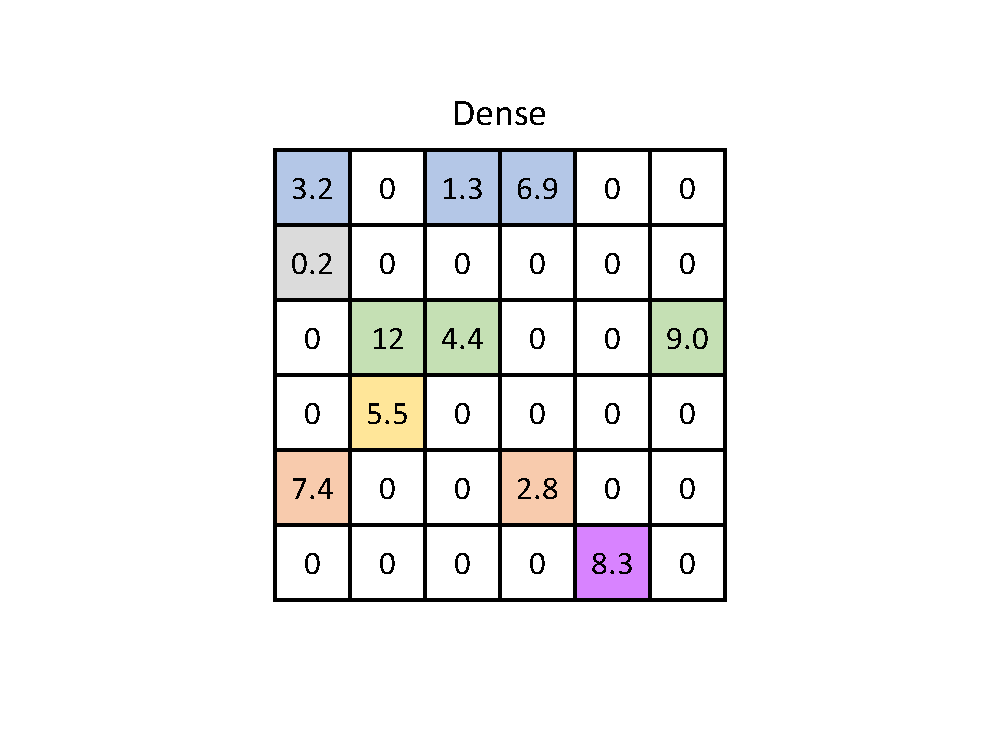
\includegraphics[page=1,width=\textwidth]{FormatDiagram.pdf}
    \caption{Dense represention of data. Nonzero entries are colored by their row value.}\label{FormatDiagram:Dense}
  \end{subfigure}
  \begin{subfigure}{0.45\textwidth}
    \includegraphics[page=2,width=0.95\textwidth]{FormatDiagram.pdf}
    \caption{Coordinate storage represention of data. Nonzero entries are colored by their row value.}\label{FormatDiagram:COO}
  \end{subfigure}

  \begin{subfigure}[c]{0.45\textwidth}
    \includegraphics[page=3,width=0.95\textwidth]{FormatDiagram.pdf}
    \caption{Compressed sparse row represention of data. Nonzero entries are colored by their row value.}\label{FormatDiagram:CSR}
  \end{subfigure}
\caption{Dense, COO, and CSR storage representations of the same data.}\label{FormatDiagram}
\end{figure*}

Listing~\ref{DenseAndSparseMV} shows C-like implementations of the SpMV kernel using dense and sparse data formats.
The first implementation shows the computation written for a dense matrix.
The second implementation shows the computation written for coordinate storage (COO). 
In this format, the View contains three vectors: one for the row indices, one for the column indices, and one for the nonzero values.
These vectors contain as many elements as there are nonzero values.
The third implementation shows the computation written for a View in compressed sparse row storage (CSR).
This storage format is based on COO, but rather than storing every element of the row vector, it is compressed to a vector of offsets that indicate the start of each row within the column and value vectors.
Figure~\ref{FormatDiagram} shos a graphical representation of the three formats.



Consider the extent to which the representations of the computations depend on the selected data format.
In the sparse implementation, the data format of \verb.A. changes not only the access to \verb.A., but also the bounds of the inner loop --- now a function of the entries of \verb.rowptr.--- and even the access to the other data in the computation (\verb.x.).
All parts of the computation description have been tied up with the format of just one of the arrays.
This means that changes to the format of \verb.A. will require modifying nearly all parts of the computation, significantly reducing the flexibility of the code.


\subsection{RAJA's Flavor of Decomposition}
The previous subsection showed how different sparse formats need to be handled when changing sparse formats by hand.  
In this subsection, I discuss RAJA's approach to decomposition and the constraints it places on my approach of providing a way to specify the sparse computation without having to rewrite the loops.

As discussed in previous chapters, a RAJA computation is broken up into a description of the operation, the iteration space, the schedule, and the data format.
The main idea of my approach is to introduce an additional component for the sparsity of the data.
Then, the problem of extending RAJA to support sparse computations is reduced to identifying how this new sparsity should interact with each of the existing components.

The operation of the computation is provided by the user as lambdas that execute the iterations of a loop. 
Because the operation involves accessing sparse data, it presents strong constraints on the design of the sparse extension. 
Most importantly, the operation of the loop nest should be written the same regardless of the format. 
The natural candidate here is the existing interface for data access in dense RAJA codes: the call operator. 
While using the call operator to support accesses to sparse data produces an attractive interface for describing a computation, it surfaces the challenge of devising an access function that traverses the sparse data efficiently throughout a computation. This problem and my solution are discussed in Section~\ref{sec:SparseAccess}.

For the iteration space, we take a similar approach of format-agnostic specification.
The programmer describes the iteration space as if its a dense code then use the sparsity of the data to exclude iteration space points that do not access nonzero data.
This can be partially automated as part of the construction of the computation object, or done ahead of time by the programmer.
The automated process involves using the access information extracted from the operation to determine which iteration space points need to be retained.

The approach of augmenting a dense-like specification continues into the description of the schedule. 
The central challenge here is related to the construction of the sparse iteration space. 
As the sparse space is created out of the dense one, its representation needs to be compact and easily traversable by RAJA's kernel execution. 

Finally is the data format, where the sparsity plays a greater role.
While I restrict the prototype to COO and CHS formats, the dimensional ordering still plays an important role.
This is because the particulars of the data storage order influence the efficency of contsructing the sparse iteration space and traversing through the data.
Regardless of the underlying representation, the layout of the sparse view supports the standard multi-dimensional indexing functions that are used to access dense data.

\subsection{Computational Complexity}

Even for computations that only executes iterations that access a nonzero value, application performance depends on the speed the sparse data can be accessed.
Without any optimizations, each access to sparse data requires searching. 
Each dimension in the index hierarchy must be searched for the corresponding value, until either the entry is found or it can be determined that the entry is a zero.
In the worst case, for a View with $D$ dimensions and $NNZ$ nonzero entries, the complexity of a single access is $O(D * \log(NNZ))$. 
This is compared to $O(D)$ for a dense View.

Requiring a search on every access to a sparse structure is prohibitively expensive, but it is possible to reduce the complexity to constant time.
Specifically, if the computation uses a schedule and format that access and store the data in exactly the same order, then the search can be avoided entirely.
Instead, the index into the View's data is updated incrementally, processing the data in order.

In implementations written by hand or with code-generating approaches, incremental updates are hard-coded into the loop's implementation, either by the programmer or the compiler.
Each format requires a unique implementation that traverses its entries in the appropriate order, so code written for one format will not work for another.
My approach incorporates parts of this incremental update technique without requiring the code to be rewritten for each desired format. 
This involves maintaining a field in the SparseView that tracks its most recent access.
Then, when accessed, the view checks if the indices are for the entry stored next in the data. 
If so, the view can bypass the searching and immediately return the desired value. 
If not, the view performs the search as to return the correct value. 
This approach, a sort of software prefetching, does incur the overhead of a comparison between the current access and the expected access, but this $O(D)$ check is much faster than the $O(D*\log(NNZ))$ search.
The hypothesis is that, with sufficient optimization, this approach can provide comparable performance to a hand-implemented version of the code.

\section{Constructing a Sparse Iteration Space}\label{sec:sparseIterspace}
Omitting unnecessary iterations is key to the performance of a sparse computation. 


The first performance barrier for SparseRAJA is the representation and construction of the sparse iteration space.
While individual dimensions in a RAJA iteration space can be ranges (using \verb.RangeSegment.) or arbitrary lists (using \verb.ListSegment.), dimensions can only be combined using the cartesian product. 
This presents a problem, as scarcely any sparse iteration spaces can be represented as a cartesian product.
Another option is needed, and here, I explore two.


\subsection{Option 1: Specialized Iterators}
The leader/follower iterator approach requires no changes to the kernel policy, but is limited in the scheduling orders in can support. 
At a high level, the iterators for each loop dimension are synchronized, traversing a zipped list rather than a cartesian product. 
Because this method incorporates the synchronization through the segments themselves, it does introduce some runtime overhead.

When constructing the sparse iteration space, the outermost segment is created as a \verb.LeaderSegment. object and the inner segments are created as \verb.FollowerSegment. objects.
The inner \verb.FollowerSegment. objects store a reference to the lead segment with which they will synchronize.
Using this reference, the follower segments instantiate inner loops of length one, containing only the value in the synchronized position. 
This has the effect of compressing the multi-dimensional loop nest into a 1 dimensional loop nest traversing all the dimensions together.

Note that in this form, the approach can only support perfectly nesting schedules.
This becomes clear with an example.
Consider the following code, which accumulates the row sums of a sparse matrix into the dense vector \verb.y..:
\begin{figure}
\begin{lstlisting}
using POLICY=KernelPolicy<
  statement::For<0,
    statement::Lambda<0>,
    statement::For<1,loop_exec,
      statement::Lambda<1>
    >
  >
>;

auto init_lam = [=](auto i) {
  y(i) = 0.0;
}
auto accum_lam = [=](auto i, auto j) {
  y(i) += A(i,j);
}

auto i_dim = LeaderSegment(  {0,0,1,2,4,4,4,7});
auto j_dim = FollowerSegment({1,8,0,2,3,4,7,9});

kernel<POLICY>(make_tuple(i_dim,j_dim), init_lam, accum_lam);
\end{lstlisting}
\end{figure}
The correct behavior of this loop would be to zero out \verb.y(0)., then add to it \verb.A(0,1). and \verb.A(0,8)..
Next, it would zero out \verb.y(1). and add to it \verb.A(1,0)..
This process should continue, summing one value into \verb.y(2)., three values into \verb.y(4)., and finally one value into \verb.y(7)..

However, using this version of the leader/follower formulation, a different behavior emerges.
Because all iterator incrementing happens in the leader segment's loop level, the contents of \verb.y. are zeroed each time.
\verb.y(0). is zeroed, then \verb.A(0,1). is added.
Then \verb.y(0). is zeroed and \verb.A(0,8). is added.
This repeats with each point in the iteration space, constantly overwriting the output. 
This problem can be resolved, using a refinement discussed in the subsection after next.

\subsection{Option 2: Loop Flattening}

The second option, loop flattening, approaches the problem from the direction of the kernel policy rather than the iteration space objects themselves.
Here, a new policy statement type is introduced: \verb.FlatFor.. 
It functions similarly to the \verb.For. statement policy, but rather than iteration a single segment, it iterates multiple simultaneously. 

Because this approach changes the kernel policy, a template parameter, it is less amenable to runtime modifications. 
Furthermore, it more strictly encodes the data layout into the schedule, making it more costly to change the computation to use a different format.
However, it would incur less overhead during kernel execution than the Leader/Follower Iterators approach, as it avoids the code associated with traversing the length one inner loop nests.

An additional drawback of this approach is that it only supports perfect nesting for the dimensions that it flattens. 
This means that a loop nest that uses additional statements to initialize data or write temporaries back to memory either before or after the second nesting level cannot be represented using the \verb.FlatFor. approach.
Because of these drawbacks, I use a modified leader/follower iterator approach in the prototype, but an approach that combines the two may be the most effective.

\subsection{Compressed Leader/Follower Iterators}

The chosen approach refines the basic leader/follower iterator approach and lays the foundation for supporting compressed formats like CSR and CSC.

Rather than doing all incrementing within the leader iterator and having the follower iterators traverse a length one segment, the leader segment compresses its dimension in the style of the CSR row pointer, and the follower iterators traverse variable length segments based on the number of nonzeros that share the same leader iterator value.
This modified approach essentially constructs the CSR compressed dimension as part of the execution.
This approach is perfect for loops that have initialization and finalization statements, such as the summing loop nest discussed above. 


\section{Traversing Sparse Data Efficiently}\label{sec:SparseAccess}

Even with the iteration space reduced to only the necessary points, acceptable performance depends on traversing the sparse data structures efficiently without requiring a search on each access.
Here, the tradeoff is between flexibility in supporting types of computations and the performance benefits of more aggressive specialization.

\subsection{Option 1: ``Expected Next Access'' Cache}

The most flexible approach is something akin to software prefetching, based on the assumption that data will be accessed in order. 
With this approach, before an access reverts to a search of the sparse data, it checks if the current access is for the next nonzero in the View.
If so, it skips the search and immediately returns the value.
If not, it searches the View for the desired value.

While this approach incurs the cost of checking the access against the expected, it avoids the much more expensive cost of searching the entire data structure each time teh View is read or written.
Additionally, it only needs a snigle access function, avoiding the type manipulation of the other options, and supports correct execution for all kernels, regardless of data access patterns.
Listing~\ref{expectedAccessImpl} shows a possible implementation of such an access function.
\begin{figure}
\begin{lstlisting}[caption={Possible implementation fo the Expected Next Access approach to efficient data traversal.},label=expectedAccessImpl]
ElementType access(auto i0, auto i1) {
  static int expectedIdx = 0;
  if (i0 == dims[0][expectedIdx] && i1 == dims[1][expectedIdx]) {
    return values[expectedIdx++];
  }
  
  entryIndex = search(i0,i1);
  if (entryIndex == -1) {
    return 0;
  } else {
    expectedIdx = entryIndex+1;
    return values[entryIndex];
  }
}
\end{lstlisting}
\end{figure}

This approach can also be used to skip searching on accesses to coordinates with zero values.
For example, if the current access is lexicographically greater than the previous access and lexicographically less than the expected one, it can be inferred that the access should return zero. This is useful in computations that make stencil accesses.

\subsection{Option 2: Specialized Traversal Layouts}
For a certain class of kernels, where there is only one access to a sparse View, and the schedule traverses that data in order, a different approach could remove the check present in the first approach.

In this approach, each format has two implementations. 
One implementation performs a random access search, while the other traverse the data in order. 
If a programmer indicates the data will be traversed in order, or the runtime system can prove that it will, the View can be switched to the fast access format before kernel execution.

This approach has the benefit of faster access times at the cost of a smaller domain of possible kernels it could uspport. 
For example, it could not support a kernel that makes two accesses to the same View or one that makes multiple traveresals of the data, such as a matrix multiplication.

Abbreviated implementations of the formats are shown in Listing~\ref{specializedLayoutsImpl}.
\begin{figure}
\begin{lstlisting}[caption={Abbreviated format implementation for the Specialized Traversal Layout approach.},label=specializedLayoutsImpl]
class FastCOO {
  int currIdx = 0;
  \dots
  void preKernelLaunch() {
    currIdx = 0;
  }
  ElementType access(Idxs...indices) {
    return values[currIdx++];
  }
}
\end{lstlisting}
\end{figure}

\subsection{Option 3: Specialized Index Types}
The third option, like the second, uses an approach of dispatching to different access functions based on access pattern information.
Here, rather than using the View's layout type to select the access function, I use the type of the loop index values passed to the lambdas.
For example, the COO format may have two access functions, specialized for different inputs.
Listing~\ref{specializedIndexImpl} shows possible access functions fro the COO format.

This approach has the benefit of maintaining a single View layout type, avoiding the virtualization necessary to support the second approach.
This removes yet another source of overhead in the sparse access functions.
However, because it changes the type of the indexing variables, it imposes some of the same limitations as the symbolic evaluation functionality. 
Critically, all the data structures used in a kernel would need to support the different index types. 
For codes that only used dense and sparse Views, this is less of a problem.
For codes that access vectors or traditional arrays, this presents more serious issues.
Additionally, if two sparse Views are used in the same kernel, they both need to traverse their data in the efficient order.
This is because the same index type has to be used for both sparse Views.


\begin{figure}
\begin{lstlisting}[caption={Reference implementation for the Specialized Index Types approach.}, label=specializedIndexImpl]

ElemetType access(int i0, int i1) {
  return searchAccess(i0,i1);
}
int fastIdx = 0;
ElementType access(FastIdx i0, FastIdx i1) {
  return values[fastIdx++];
}
\end{lstlisting}
\end{figure}

\subsection{Striking a Balance}
While the latter two options offer the potential for better performance than the first, it comes at a steep price of applicability.
For this reason, I use the expected next access approach in the prototype.
Certain computations present a challenge for all three approaches, such as the multiplication of a sparse matrix with its transpose.
Support for efficient traversal in such a computation is a direction for future research, and likely relies on maintaining multiple copies of the data structure, stored in different orders.
Such an approach could also mantain multiple expected access checks, one for each of the two storage directions.

\section{Prototype Implementation}

I implemented the approaches discussed in the previous two sections into a prototype for sparse computation support within RAJA.~
Here, I discuss the interface and algorithms for constructing sparse data structures, iteration spaces, and computations.
% Constraints
% \begin{itemize}
% 	\item Conditional statements within loop bodies must not contain View accesses in their conditional expression.
% 	\item View indexing expressions must be lone iterators rather than affine expressions of the iterators, as in previous chapters.
% 	\item All writes to sparse Views must be updates, not insertions of new nonzeros.
% \end{itemize}

\subsection{Sparse Data Containers}

With the prototype's limitation to coordinate storage, two functions support the creation of sparse views: \verb.make_sparse_view. and \verb.make_permuted_sparse_view..
The former is a wrapper of the latter, generating a SparseView with the identity permutation.
For an $N$ dimensional SparseView, there are $N+2$ parameters to \verb.make_permuted_sparse_view..
The first $N$ parameters are vectors containing the index values for each dimension. 
This means that for a 2 dimensional SparseView, the first two arguments are the row and column indices of the entries.
The $N+1th$ parameter is a vector containing the entries themselves. 
Finally, the last parameter is the permutation vector for the SparseView. 
The idea of the permutation vector is that it changes how the entries of the view are sorted, but not how they are referenced / indexed.

Consider a sparse view containing the following entries, presented here unordered:
\begin{lstlisting}
DIM0: 0 1 2 1 0 2
DIM1: 1 1 0 2 2 0
DIM2: 1 0 2 1 0 0
VAL : A B C D E F 
\end{lstlisting}
If these entries are used to construct the standard SparseView, they will be reordered and stored as follows:
\begin{lstlisting}
DIM0: 0 0 1 1 2 2
DIM1: 1 2 1 2 0 0
DIM2: 1 0 0 1 0 2
VAL : A E B D F C
\end{lstlisting}
If the SparseView is constructed with the permutation vector $(2,0,1)$, they will be stored as:
\begin{lstlisting}
DIM0: 0 1 2 0 1 2
DIM1: 2 1 0 1 2 0
DIM2: 0 0 0 1 1 2
VAL : E B F A D C
\end{lstlisting}
Note that the list of dimensions is not permuted, only the order the entries are sorted. 
What this scheme means is that no matter the permutation, the access \verb.view(0,1,1). will always return \verb.A., even if its location in the list of entries changes.

The nonzero pattern of the SparseView data type is a read-only feature in the prototype.
This is not an inherent limitation, but additional considerations must be taken into account when designing mutable sparse data structures.
For example, because the iteration space of a sparse computation is based on the nonzero structure of the SparseView used in it, inserting new nonzeros into a SparseView during a computation could change the computation's iteration space as it is executing.
Additionally, the cost of inserting elements one at a time can be quite high. 
Thus, it is usually preferable to create a buffer of elements to insert and update the data structure all at once.
This buffer can take the form of a hash table which is emptied into the SparseView periodically.
With this in mind, it is possible to update the values of existing nonzero values within SparseViews, as this does not require inserting new elements into the data structure.

The SparseView class is templated by three values: the element type, the number of dimensions, and the type of the Format.
\verb.make_sparse_format. has an optional template parameter for choosing different formats, defaulting to coordinate storage.
The SparseView class wraps the templated sparse format type and manages a symbolic evaluation itself.
Most of its methods directly forward to calls of the format implementation class.
A programmer can easily create a new sparse format by creating an implementation class that implements a small collection of functions.
Most important is the call operator, but also necessary are functions for accessing individual dimension index values, the number of nonzero entries, and diagnostic functions for examining the expected access cache hit rates.

\subsection{Sparse Iteration Spaces}
The implemented algorithm for automatically constructing the sparse iteration space from the dense iteration space and a sparse data access addresses the common case.
It assumes the iteration space dimensionality and the data space dimensionality are equal, and is based on an access to the sparse data that uses each loop iterator once.

The idea of the algorithm is to construct the sparse iteration space out of the dimensions of the SparseView. 
First, the dimensions of the iteration space are matched to the dimensions of the SparseView based on the access information gathered from the symbolic evaluation.
For example, the accesses \verb.A(i,j). and \verb.A(j,i). match the first dimension of the SparseView to the first and second dimensions of the iteration space, respectively.
Second, the lead dimension, traversed by the outermost \verb.For. statement, is constructed using the relevant SparseView dimension.
This requires that the SparseView is sorted by this dimension on the first level.
Once this is complete, the follow dimensions are constructed for the remaining dimensions of the SparseView.
Listing~\ref{sparsifyAlg} shows a pseudo-code implementation of the algorithm.
\todo{update algorithM}.

\begin{figure}
\begin{lstlisting}[caption={Abbreviated algorithm for sparsifying a dense iteration space.}, label=sparsifyAlg]
auto sparsify(IterationSpace denseSpace, SparseAccess access) {
  auto q = invert(access.orderPermutation);
  auto view = access.accessedView;

  auto sparseRect = [];
  auto leadDimension = SparseSegmentLead(view, q[0]);
  sparseRect.push_back(leadDimension);
  for(int i = 1; i < view.numDims; i++) {
    auto dim = SparseSegmentFollow(view, q[i], &leadDimension);
    sparseRect.push_back(dim);
  }
  return IterationSpace(sparseRect, denseSpace.constraints);
}
\end{lstlisting}
\end{figure}

\subsection{Sparse Kernel Objects}

The automatic construction of a sparse iteration space is surfaced to the user through the \verb.make_sparse_kernel. function.
An extension of the existing \verb.make_kernel. function, the sparse variant includes two extra parameters (one optional, one required) used to construct the sparse iteration space.
First is the required runtime parameter for the sparse View that the iteration space should be constructed around.
This parameter comes after the dense iteration space and before the lambdas for the loop bodies.
Second is an optional template index parameter, specifying which of the lambdas should be evaluated symbolically to gather the access information necessary for creating the new iteration space.
An abbreviated implementation is shown in Listing~\ref{makeSparseKernelAlg}.

When called, \verb.make_sparse_kernel. starts by symbolically evaluating the specified lambda.
This collects all access information, for both sparse and dense Views.
The next step isolates the accesses to the sparse View guiding the construction by a standard search.
This access, the kernel policy, and the dense iteration space are then used to construct the sparse iteration space.
The final step is to return a KernelWrapper that will execute the computation over the newly constructed sparse iteration space.

\begin{figure}
\begin{lstlisting}[caption={Abbreviated implementation of the function for creating a computation that automatically constructs the sparse iteration space.}, label=makeSparseKernelAlg]
template <typename KernelPolicy, idx_t SymExecLamIdx=0>
auto make_sparse_kernel(auto denseSegs, auto sparseView, auto loopBodyTuple) {
  auto symExecLambda = get<SymExecLamIdx>(loopBodyTuple);
  auto allAccesses = symbolically_evaluate(symExecLambda);
  auto sparseAccess = findAccessTo(sparseView, allAccesses);

  auto sparseSegs = make_sparse_iteration_space<KernelPolicy>(denseSegs, 
  sparseAccess);

  return make_kernel<KernelPolicy>(sparseSegs, loopBodyTuple);
}
\end{lstlisting}
\end{figure}

Alternatively, the programmer can construct the sparse iteration space themselves, then use the standard \verb.make_kernel. to generate the computation over the sparse iteration space.

\section{Evaluation}\label{sec:sparseEval}
To evaluate the prototype, I compare the performance of different versions of three benchmarks: sparse matrix vector multiplication (SpMV), Gauss-Seidel iteration (GauSei), and incomplete Cholesky factorization (InCholFact).
The first version, \dense, implements the computation on dense data. 
The second version, \specialized, is specialized for a particular sparse format by hand. 
The third version, \sparseraja, implements the computation using the prototype support described above.
In terms of representation, the expectation is that the \dense{} and \sparseraja{} versions of the code will look similar, both varying significantly from the format-specific implementation of the \specialized{} version.
In terms of performance, the \dense{} version is expected to be the outlier, as it executes many more iterations than the \sparseraja{} and \specialized{} versions.

The evaluation process here is iterative, progressing through a loop of running the evaluation, profiling using hpctoolkit~\cite{adhianto2010hpctoolkit}, identifying potential optimizations, and implementing them. 
This is in service of evaluating the overall question of the feasibility of acheiving comparable performance to the hand-specialized variants.





\subsection{Benchmark 1: SpMV}
While a relatively simple computation on its own, sparse matrix vector multiplication (SpMV) is a foundational building block for sparse computations.
The computation has two pieces of input data: a sparse matrix \verb.A. and a dense vector \verb.x.. 
Each element of the single output vector \verb.y. is the dot product of the corresponding row of \verb.A. with the whole vector \verb.x..
Listings~\ref{DenseMV},~\ref{SpecializedMV}, and~\ref{SparseRAJAMV} show the reference implementations for the three versions of the computation.


\begin{figure}
\begin{lstlisting}[caption={RAJA implementation of dense matrix vector multiplication.},label=DenseMV]
DenseView<1> x(Nj);
DenseView<1> y(Ni);
DenseView<2> A(Ni,Nj);

using POLICY = KernelPolicy<
  statement::For<0,loop_exec,
    statement::For<1,loop_exec,
      statement::Lambda<0>
    >
  >
>;

auto seg1 = RangeSegment(0,Ni);
auto seg2 = RangeSegment(0,Nj);
auto segs = make_tuple(seg1, seg2);

auto lam = [&](auto i, auto j) {
  y(i) += A(i,j) * x(j);
};

auto knl = make_kernel<POLICY>(segs, lam);
knl();
\end{lstlisting}
\end{figure}
\begin{figure}
\begin{lstlisting}[caption={RAJA implementation of sparse matrix vector multiplication, specialized for COO storage.},label=SpecializedMV]
DenseView<1> x(Nj);
DenseView<1> y(Ni);
DenseView<1> A_cols(NumNonZeros);
DenseView<1> A_rows(NumNonZeros);
DenseView<1> A_vals(NumNonZeros);

auto seg = RangeSegment(0,NumNonZeros);

auto lam = [&](auto idx) {
  auto i = A_rows(idx);
  auto j = A_cols(idx);
  y(i) += A_vals(idx) * x(j);
};

auto knl = make_forall<loop_exec>(seg, lam);
knl();
\end{lstlisting}
\end{figure}
\begin{figure}
\begin{lstlisting}[caption={Implementation of SpMV using the SparseRAJA prototype},label=SparseRAJAMV]
DenseView<1> x(Nj);
DenseView<1> y(Ni);
SparseView<2> A(Ni,Nj);

using POLICY = KernelPolicy<
  statement::For<0,loop_exec,
    statement::For<1,loop_exec,
      statement::Lambda<0>
    >
  >
>;

auto seg1 = RangeSegment(0,Ni);
auto seg2 = RangeSegment(0,Nj);
auto dense_segs = make_tuple(seg1, seg2);

auto lam = [&](auto i, auto j) {
  y(i) += A(i,j) * x(j);
}

auto knl = make_sparse_kernel<POLICY>(dense_segs, A, lam);
  
knl();
\end{lstlisting}
\end{figure}




\subsection{Benchmark 2: Gauss-Seidel Iteration}

The second kernel, Gauss-Seidel iterative solve, is a well-known kernel for approximating the solution to a linear system.
The problem of solving a linear system is thus: given a coefficient matrix $A$ and a right-hand side vector $b$, find a vector $x$ such that $Ax=b$.
The Gauss-Seidel method does this by starting with an initial guess and successively refining it to closer and closer approximations.
This process is repeated until a desired level of accuracy is reached.

While the kernel itself is applied iteratively to refine the approximation, we focus here on the operations of the iterations internal to the kernel.
An imperfectly nested, two-dimensional loop nest, GauSei updates each element of the solution vector $x$ in sequence.
First, the dot product of a row of $A$ and the current approximation is accumulated in a temporary variable.
Note that if the approximation is exactly correct, this value will be equal to the corresponding entry of $b$. 
The difference between the temporary and the right-hand side is then used to update the approximation, and the process repeats.

Gauss-Seidel is a tricky kernel because of its data dependences.
The results of earlier iterations change values used in subsequent ones, meaning that the order of the iterations cannot be changed arbitrarily. 
For this reason, GauSei cannot be represented as tensor algebraic expressions, placing it outside TACO's space of expressible computations~\cite{}.

Listings~\ref{DenseGauSei},~\ref{SpecializedGauSei}, and~\ref{SparseRAJAGauSei} show the three reference implementations of the GauSei kernel.
Because of the significant variations between the three implementations, I also show a C-like reference implementation in Listing~\ref{CppGauSei}.

One such variation appears in the \specialized{} version. 
Because specializing the implementation for the COO format flattens the iteration space from two dimensions to one, guard statements must be inserted to check for changes in rows. 
Furthermore, it also requires pulling part of the final iteration out of the loop.

\begin{figure}
\begin{lstlisting}[caption={C-like version of Gauss-Seidel iteration},label=CppGauSei]
View<2> A(N,N);
View<1> b(N);
View<1> x(N) = initial_guess;
double temp;

while(!has_converged()) {
  for(int i = 0; i < N; i++) {
    temp = 0.0;
    for(int j = 0; j < N; j++) {
      if (j != i) {
        temp += A(i,j) * x(j);
      }
    }
    x(i) = (b(i) - temp) / A(i,i);
  }
}
\end{lstlisting}
\end{figure}

\begin{figure}
\begin{lstlisting}[caption={\dense{} version of Gauss-Seidel iteration},label=DenseGauSei]
View<2> A(N,N);
View<1> b(N);
View<1> x(N) = initial_guess;
double temp;

using POLICY = KernelPolicy<
  statement::For<0,loop_exec,
    statement::Lambda<0>,
    statement::For<1,loop_exec,
      statement::Lambda<1>,
    >,
    statement::Lambda<2>
  >
>;

auto lam1 = [&](auto i) {
  temp = 0.0;
};
auto lam2 = [&](auto i, auto j) {
  if (j != i) {
    temp += A(i,j) * x(j);
  }
};
auto lam3 = [&](auto i) {
  x(i) = (b(i) - temp) / A(i,i);
}

auto seg1 = RangeSegment(0,N);
auto seg2 = RangeSegment(0,N);
auto segs = make_tuple(seg1, seg2);

auto knl = make_kernel<POLICY>(segs, lam1, lam2, lam3);

while (!has_converged()) {
  knl();
}
\end{lstlisting}
\end{figure}

\begin{figure}
\begin{lstlisting}[caption={\specialized{} version of Gauss-Seidel iteration},label=SpecializedGauSei]
View<2> A_rows(NNZ);
View<2> A_cols(NNZ);
View<2> A_vals(NNZ);
View<1> b(N);
View<1> x(N) = initial_guess;

while (!has_converged()) {
  int prev_i = 0;
  double temp = 0.0;
  for(int idx = 0; idx < NNZ; idx++) {
    int i = A_rows(idx);
    int j = A_cols(idx);
    double v = A_vals(idx);

    if (i != prev_i) {
      double prev_diagonal = find(prev_i, prev_i, A_rows, A_cols, A_vals);
      x(prev_i) = (b(prev_i) - temp) / prev_diagonal;
      temp = 0.0;
      prev_i = i;
    }
    if (j != i) {
      temp += v * x(j);
    } 
  }
  double prev_diagonal = find(prev_i, prev_i, A_rows, A_cols, A_vals);
  x(prev_i) = (b(prev_i) - temp) / prev_diagonal;
}
\end{lstlisting}
\end{figure}


\begin{figure}
\begin{lstlisting}[caption={\sparseraja{} version of Gauss-Seidel iteration},label=SparseRAJAGauSei]
SparseView<2> A(N,N);
View<1> b(N);
View<1> x(N) = initial_guess;
double temp;

using POLICY = KernelPolicy<
  statement::For<0,loop_exec,
    statement::Lambda<0>,
    statement::For<1,loop_exec,
      statement::Lambda<1>
    >,
    statement::Lambda<2>
  >
>;

auto lam1 = [&](auto i) {
  temp = 0.0;
};
auto lam2 = [&](auto i, auto j) {
  if (j != i) {
    temp += A(i,j) * x(j);
  }
};
auto lam3 = [&](auto i) {
  x(i) = (b(i) - temp) / A(i,i);
};

auto seg1 = RangeSegment(0,N);
auto seg2 = RangeSegment(0,N);
auto segs = make_tuple(seg1, seg2);

auto knl = make_sparse_kernel<POLICY, 1>(segs, A, lam1, lam2, lam3);

while (!has_converged()) {
  knl();
}
\end{lstlisting}
\end{figure}

\subsection{Benchmark 3: Incomplete Cholesky Factorization}
\begin{figure}
\begin{lstlisting}[caption={C++ reference implementation of incomplete Cholesky factorization.},label=CppInCholFact]

View<2> A(N,N);   

for(i0 = 0; i0 < N; i0++) {
  A(i0,i0) = sqrt(A(i0,i0));
  for(i1 = i0+1; i1 < N; i1++) {
    if (A(i1,i0) != 0) {
      A(i1,i0) /= A(i0,i0);
    }
  }
  for(i1 = i0+1, i1 < N; i1++) {
    for(i2 = i1; i2 < N; i2++) {
      if (A(i2,i1) != 0) {
        A(i2,i1) -= A(i2,i0) * A(i1,i0);
      }
    }
  }
}

for(i0 = 0; i0 < N; i0++) {
  for(i1 = i0+1; i1 < N; i1++) {
    A(i0,i1) = 0;
  }
}
\end{lstlisting}
\end{figure}

\todo{introduce what it does}

\todo{introduce data requirements}

\todo{discuss any notable characteristics.}

\todo{reference implementations}


\subsection{Performance Results}

\subsubsection{SpMV}
\begin{figure}
\includegraphics[width=0.5\textwidth]{SpMV_lines_perf.pdf}
\caption{Matrix vector multiplication execution times for different variants and sparse matrix densities. Each subplot charts a different dimension length. Both x and y are log scale. Lower is better.}\label{SpMVPerformance}
\end{figure}
Figure~\ref{SpMVPerformance} shows the performance evaluation results for the \SpMV{} kernel. 
The three lines represent the different variants.

For each subplot charting the results of evaluation for one dimension length, the \dense{} variant shows constant execution time across densities.
This is because it performs all iterations, even if the value in the matrix is 0.
Both the \sparseraja{} and \specialized{} variants show consistent linear scaling with density and size. 


% ./run.sh -s 64 -s 128 -s 192 -s 212 -s 256 -d 0.5 -d 0.1 -d 0.01 -d 0.001 --spmv -o results3.csv --dense --specialized --sparseRAJA
% ./run.sh -s 64 -s 128 -s 192 -s 212 -s 256 -d 0.3 -d 0.03 -d 0.2 --spmv -o results3.csv --dense --specialized --sparseRAJA --append 
% ./run.sh -s 384 -d 0.5 -d 0.1 -d 0.01 -d 0.001 -d 0.3 -d 0.03 -d 0.2 --spmv -o results3.csv --dense --specialized --sparseRAJA --append
% ./run.sh -s 512 -d 0.1 -d 0.01 -d 0.001 -d 0.3 -d 0.03 -d 0.2 --spmv -o results3.csv --specialized --sparseRAJA --append
% ./run.sh -s 512 -d 0.5  --spmv -o results3.csv --dense --append
% ./run.sh -s 64 -s 128 -s 192 -s 212 -s 256 -d 1.0 -d 0.8 --spmv -o results3.csv --specialized --append
With the first version the \sparseraja{} variant shows a geometric mean speedup of 0.103, just under a 10x slowdown.
Analysis with hpctoolkit uncovered an expensive vector allocation within the access function.
% ./run.sh -s 64 -s 128 -s 192 -s 212 -s 256 -s 384 -s 512 -d 0.5 -d 0.3 -d 0.1 -d 0.05 -d 0.025 -d 0.01 --spmv -o results4.csv --specialized --sparseRAJA
% ./run.sh -s 64 -s 128 -s 192 -s 212 -s 256 -s 384 -s 512 -d 0.5 --spmv -o results4.csv --dense --append 
Using a fixed size \verb.std::array. triples relative performance with a 0.282 geometric mean speedup, just under a 4x slowdown.
More optimization passes will be necessary to continue improving performance.
%hpcrun ./build/bin/sparseEval.exe 0 0 1 1 0 0 800 0.2
%hpcrun ./build/bin/sparseEval.exe 0 0 1 1 0 0 800 0.8
%hpcstruct -Isrc/+ build/bin/sparseEval.exe
%hpcprof -Isrc/+ -SsparseEval.exe.hpcstruct hpctoolkit-sparseEval.exe-measurements

% ./run.sh -s 64 -s 128 -s 192 -s 212 -s 256 -s 384 -s 512 -d 0.5 -d 0.3 -d 0.1 -d 0.05 -d 0.025 -d 0.01 --spmv -o results5.csv --specialized --sparseRAJA
% ./run.sh -s 64 -s 128 -s 192 -s 212 -s 256 -s 384 -s 512 -d 0.5 --spmv -o results5.csv --dense --append 

%./run.sh -s 1000 -d 0.8 --spmv --sparseRAJA --append --profile -o profiling3


% ./run.sh -s 64 -s 128 -s 192 -s 212 -s 256 -s 384 -s 512 -d 0.5 -d 0.3 -d 0.1 -d 0.05 -d 0.025 -d 0.01 --spmv -o results6.csv --specialized --sparseRAJA
% ./run.sh -s 64 -s 128 -s 192 -s 212 -s 256 -s 384 -s 512 -d 0.5 --spmv -o results6.csv --dense --append 
One unexpected result is that even with a density of 1, indicating a completely dense array, the specialized COO variant still outperforms the dense View. 
This may be caused by specialized version doing a simpler 1 dimensional index calculation.



\subsubsection{GauSei}
\begin{figure}
  \includegraphics[width=\textwidth]{GauSei_lines_perf_COO.pdf}
  \caption{Gauss-Seidel iteration execution times for different variants and sparse matrix densities. Each subplot charts a different dimension length. Both x and y are log scale. Lower is better. The sparseRAJA variant uses standard coordinate storage.}\label{GauSeiPerfCOO}
\end{figure}
\begin{figure}
\includegraphics[width=\textwidth]{GauSei_ratios_perf_COO.pdf}
\caption{Ratio of \sparseraja{} variant execution time to \specialized{} variant execution time. Each subplot charts a different dimension length. Lower is better. Values greater than 1 indicate that the \sparseraja{} variant is slower. The \sparseraja{} variant uses standard coordinate storage.}\label{GauSeiRatioCOO}
\end{figure}

\begin{figure}
\includegraphics[width=\textwidth]{GauSei_lines_perf_DIAG.pdf}
\caption{Gauss-Seidel iteration execution times for different variants and sparse matrix densities. Each subplot charts a different dimension length. Both x and y are log scale. Lower is better. The \sparseraja{} variant uses the prototype DIAG format.}\label{GauSeiPerfDIAG}
\end{figure}
\begin{figure}
\includegraphics[width=\textwidth]{GauSei_ratios_perf_DIAG.pdf}
\caption{Ratio of \sparseraja{} variant execution time to \specialized{} variant execution time. Each subplot charts a different dimension length. Lower is better. Values greater than 1 indicate that the \sparseraja{} variant is slower. The \sparseraja{} variant uses standard coordinate storage.}\label{GauSeiRatioDIAG}
\end{figure}
Figure~\ref{GauSeiPerfCOO} shows the initial performance of the SparseRAJA implementation using the COO storage format.
Figure~\ref{GauSeiRatioCOO} shows the ratio of the SparseRAJA variant execution time to the specialized variant execution time.
The geometric mean speedup of the SparseRAJA version relative to the specialized version is $0.228$, between a 4 and 5x slowdown. 
From the early profiling rounds of the \GauSei{} kernel, nearly 90\% of the execution time is spent in the SparseView's search-based random access function.
This is caused by the comparatively low expected access cache hit rate, driven by the irregular access patterns in the kernel.
First, each of the diagonal entries is skipped during the execution of the inner loop nest.
After each diagonal iteration, where no access is made because the conditional is false, the expected access is still the diagonal entry. 
Thus, the following iteration will access the entry after the diagonal and have to search.
Second, each diagonal is accessed after the row is processed in the finalizing statement.
This causes two misses, one when the finalizing statement executes and the access to the diagonal entry is made, then another on the first inner iteration of the next row, attempting to access the first entry of the row.
Barring the occasional circumstance where the diagonal is the last or only value in the row, there are three misses for each row in the input matrix.

Here we encounter a situation where a different data format would be beneficial.
For example, a format that additionally stores a vector of the diagonal entries separately from the other entries.
On an access, if the access is for a diagonal, it indexes directly into the vector, otherwise following the usual pattern of prefetching and searching.
Figure~\ref{GauSeiPerfDIAG} shows the perforamnce of a variant using this DIAG storage format instead of the general COO format compared to the specialized hand-implemented variant.
Here, the geometric means speedup is $0.182$, between a 5 and 6x slowdown, and slower than the coordinate storage variant. 
This may be caused by the additional overhead of checking each if each access is to the diagonal.


\section{Conclusion}

This chapter explored incorporating support for sparse computations and data formats into the RAJA performance portability library.
By treating the sparsity of the data as an independent component of the computation's specification, the approach enables concise and format-independent programming. 
However, the overhead of maintaining and updating the necessary data structures for kernel execution, especially updating the sparse iterative values, caused performance to suffer.
While this approach may be feasible as a foundation for introducing schedule and data transformations for sparse computations, more work is needed to bring the performance of the system within the range of hand-implemented versions.







% \subsection{Computation Interface}

% The driving concern for the interface is that the details of which sparse formats the Views are stored in should be abstracted out of the computation description as much as possible. 
% This means that the description of a sparse computation should look very similar to that of a dense computation. 

% I introduce a new computation wrapper type, \verb.SparseKernelWrapper. to visually indicate that the computation should consider the sparsity of the data. 
% Like the original \verb.KernelWrapper. type, I also introduce a \verb.make_sparse_kernel. function for creating sparse computation objects. 



% \begin{figure}
% \begin{lstlisting}

% \end{lstlisting}
% \end{figure}



% \subsection{Sparsifying the Iteration Space}

% Once the computation object has been created, the sparsity of its data must be used to reduce the iteration space to only the points where nonzero datapoints exist.
% My approach proceeds in two phases: a symbolic representation phase and a execution phase. 


% \begin{figure}
% \begin{lstlisting}[caption={Algorithm to sparsify iteration space based on access to SparseView}]
% haveCompressed = false;
% compressedDim = -1;
% for nest in nesting:
% 	if nest not in access:
% 		sparseSegs[nest] = segs[nest];
% 	else if haveCompressed:
% 		idx = access.indexOf(nest);
% 	sparseSegs[nest] = segs[nest] & view.dense_by(idx, compressedDim);
% 	else:
% 		idx = access.indexOf(nest);
% 		sparseSegs[nest] = segs[nest] & view.compressed(idx);
% 		haveCompressed = true;
% 		compressedDim = idx;

% return sparseSegs;
% \end{lstlisting}
% \end{figure}


% \subsection{Efficient Iteration Through Data}


% \subsection{Permuted Coordinate Sparse Views}


% The interaction between RAJA kernel policy execution and the permuted data structure creates a challenge. 
% I turn now to a short investigation of RAJA kernel policies to elucidate this challenge.

% \subsection{Kernel Policies for Sparse Computations}

% I begin this investigation with the following two dimensional kernel:
% \begin{lstlisting}
% using POLICY = KernelPolicy<
%   statement::For<0,seq_exec,
%     statement::For<1,seq_exec,
%       statement::Lambda<0>
%     >
%   >
% >;

% auto segments = make_tuple(RangeSegment(0,2), RangeSegment(3,5));

% kernel<POLICY>(segments, [=](auto i0, auto i1) {
%   std::cout << i0 << "," << i1 << "  ";
% });
% \end{lstlisting}
% From this kernel, we would expect the output to be \verb.0,3  0,4  1,3  1,4..

% Next, consider the same kernel with the following slightly modified kernel policy:
% \begin{lstlisting}
% using POLICY = KernelPolicy<
%   statement::For<1,seq_exec,
%     statement::For<0,seq_exec,
%       statement::Lambda<0>
%     >
%   >
% >;
% \end{lstlisting}
% With this policy, the outer for loop will increment the second segment and the inner loop will increment the first.
% Thus, the expected output would be \verb.0,3  1,3  0,4  1,4..

% Finally, consider a different modification to the kernel policy:
% \begin{lstlisting}
% using POLICY = KernelPolicy<
%   statement::For<0,loop_exec,
%     statement::For<1,loop_exec,
%       statement::Lambda<0>
%     >
%   >
% >;
% \end{lstlisting}
% Here, the loop-level execution policies have changed from \verb.seq_exec. to \verb.loop_exec..
% And while this has changed, we still would expect the output to be \verb.0,3  0,4  1,3  1,4..
% So what has changed? 
% Something quite subtle about the semantics. 
% The \verb.seq_exec. policy demands \enquote{strictly sequential execution,} whereas \verb.loop_exec. \enquote{allow[s] the compiler to generate any optimizations that its heuristics deem beneficial}~\cite{rajadocs}.

% Now, why is this relevant? 
% It is relevant because these concepts must be mapped to sparse computation in a way that is intuitive but still enables efficient execution on the backend.
% So the question here is: what constraints on the sparse schedule are imposed by the use of policies with either \verb.seq_exec. or \verb.loop_exec.?

% One thing is somewhat clear: regardless of the loop-level execution policy, kernel execution should be implemented as two nested for loops. 
% Further, the for loops should traverse the dimensions indicated in the policy. 
% This means the difference between \verb.loop_exec. and \verb.seq_exec. is constrained to an individual loop level. 

% Once more, why is this relevant? 
% The relevance comes from the the task of sparsifying an iteration space when the traversal order of the iteration space does not match the storage order of the sparse data.
% If the iteration space traversal order is a strict constraint, then there are two options.
% Either we reorder the sparse data to match the traversal order, or we perform a \enquote{trivial sparsification,} returning the original dense iteration space.

% \subsection{A Constraint of Idiomatic RAJA}

% The challenge of the previous subsection uncovers a constraint imposed by the RAJA library's design.
% RAJA's execution strategy is based on the enumeration of a cross product. 
% Every combination of values in the segments is visited.
% For a sparse iteration space, this approach fails.
% Rather than enumerating a cross product, a sparse computation must iterate over each dimension simultaneously. 
% The values of $j$ when $i=0$ are different from the values of $j$ when $i=1$. 

% The core of the problem here is that the inner dimensions of a loop must not be static. 
% They must be able to change as the outer iterators change.

% \subsection{Another Problematic Example}

% Consider the following kernel for a square, sparse matrix \verb.A. in the unpermuted COO format:
% \begin{lstlisting}

% using POLICY = KernelPolicy<
%   statement::For<0, loop_exec,
%     statement::For<1, loop_exec,
%       statement::Lambda<0>
%     >
%   >
% >;
% auto segments = make_tuple(seg, seg);
% auto lam = [&](auto i, auto j) {
%   z(i) += A(i,j) * y(j);
% }

% kernel<POLICY>(segments, lam);
% \end{lstlisting}
% In this computation, we have a nesting order $(0,1)$, a layout order $(0,1)$, and an access order $(0,1)$. 
% We can sparsify the iteration space without changing the layout.

% Now, what if we were to change the access order? 
% \begin{lstlisting}
% auto lam2 = [&](auto i, auto j) {
%   z(i) += A(j,i) * y(j);
% }
% \end{lstlisting}
% Now, the access order has changed from $(0,1)$ to $(1,0)$. 
% The $(i,j)$th iteration is no longer accessing the $(i,j)$th element of \verb.A. 
% When we sparsify an iteration space, we must maintain all iterations where a nonzero element is accessed. But we must remove the unnecessary iterations without reordering the remaining.
% So in this case, we have the following iteration space ${[i,j] | A[j,i] != 0}$
% Before considering how it is to be calculated, we can observe that for efficient iteration, the data in \verb.A. must be sorted in the order $(1,0)$. 
% This is because the inner loop is indexing the first dimension of \verb.A. and the outer loop is indexing the second dimension. 

% Changes to the layout order do not change the semantics. Changes to the access order and nesting order do change the semantics.

% \subsection{Sparsifying the Iteration Space}

% We begin with the case of an iteration space and square view with equal dimensionality.
% Let the iteration space be $I = \{[i_0,i_1,...,i_n] | C\}$ for some constraints $C$.
% We seek to sparsify based on an access $A(i_{p(0)},i_{p(1)},...i_{p(n)})$ for a permutation $p$.
% This is equivalent to calculating the set $I_s = \{[i_0,i_1,...,i_n] | C \land A(i_{p(0)},i_{p(1)},...i_{p(n)}) \neq 0\}$.

% Let $E_A$ indicate the indices of the nonzeros entries of $A$. 
% Formally, $E_A = \{[i_0,i_1,...,i_n] | A(i_0,i_1,...,i_n) \neq 0\}$.
% Claim: for the identity permutation $p$, $E_A = I_s$.

% Proof: => 
% consider $e = [e_0,e_1,...,e_n] \in E_A$. 
% Because it is in $E_A$, we have $A(e) \neq 0$.
% Thus, if $e$ satisfies the constraints $C$, the $e$ is an element of $I_s$.
% Square view and iteration space, so it must.

% Proof: <=
% Consider $i$ in $I_s$. 
% We thus have $A[p(i)] \neq 0$.
% Because $p$ is the identity permutation, we have $p(i) = i$, so $A[i] \neq 0$, so $i \in E_A$.

% Next, let's turn to an arbitrary permutation $p$. 
% Again let $q$ be the inverse permutation of $p$. 
% Claim: $q(E_A) = I_s$.

% Proof: => 
% consider $e = [e_0,e_1,...,e_n] \in q(E_A)$.
% If we apply the permutation $p$, we have $p(e) \in p(q(E_A))$.
% Thus, $[e_{p(0)},e_{p(1)},...,e_{p(n)}] \in p(q(E_A)) = E_A$, as $p$ and $q$ resolve to the identity permutation.
% Then, by the definition of $E_A$, we have $A(e_{p(0)},e_{p(1)},...,e_{p(n)}) \neq 0$. 
% Thus, if $p(e)$ satisfies constraints $C$, $p(e) \in I_s$. 

% Proof: <=
% consider $i = [i_0,i_1,...,i_n] \in I_s$. 
% By the definition of $I_s$, we have $A(i_{p(0)},i_{p(1)},...,i_{p(n)}) \neq 0$.
% This means that $p(i) \in E_A$.
% Finally, applying the permutation $q$ gives $q(p(i)) \in q(E_A)$, or $i \in q(E_A)$.

% Let's do an example to make this more concrete.
% Three dimensional iteration space $I = [0,N]^3$.
% Access to sparse data $A(i_2,i_0,i_1)$. 
% So $p=(2,0,1)$.
% The inverse of this permutation is $q=(1,2,0)$.
% We're looking for the set $I_s = \{[i_0,i_1,i_2] | A(i_{p(0)},i_{p(1)},i_{p(2)}) \neq 0\}$. 
% Simplified with the definition of $p$, $I_s = \{ [i_0,i_1,i_2] | A(i_2,i_0,i_1) \neq 0\}$.

% Say that $A$ has the following data:
% \begin{lstlisting}
% dim0 = {0,0,0,1,1,2,2};
% dim1 = {1,2,2,1,2,0,0};
% dim2 = {0,0,2,0,1,1,2};
%    v = {1,2,3,4,5,6,7};
% \end{lstlisting}
% Consider the data point at $(0,1,0)$ holding value $1$. 
% On iteration $(1,0,0)$, the access made will be to $A(0,1,0)$.
% On iteration $(0,1,2)$ the access will be made to $A(2,0,1)$.
% So to go from iteration to access, we apply $p$. 
% To go from access to iteration, we apply $q$.
% Since we want to calculate the iteration space points that access data in $A$, we want to apply $q$ to the data space of $A$.

% While the nesting order of a kernel changes the schedule of the execution, it does not change which points are actually in the iteration space.
% Thus, the procedure of applying the inverse permutation of the access order to the data space will produce the sparsified iteration space, which can then be scheduled using the nesting order.

% With the case of square, size-matched iteration and data spaces, let's expand to the case of a nonsquare iteration and data spaces.
% For a concrete example, let's consider the iteration space $I = \{[i_0,i_1,i_2] | 0 \leq i_0 \leq N_0 \land i_0 \leq i_1 \leq N_1 \land i_0 \leq i_2 \leq i_1 \}$.
% Let's sparsify this space based on the access $A(i_2,i_1,i_0)$. 
% The access permutation $p=(2,1,0)$, and its inverse is the same.
% The set we want to calculate is $I_s = \{[i_0,i_1,i_2] | 0 \leq i_0 \leq N_0 \land i_0 \leq i_1 \leq N_1 \land i_0 \leq i_2 \leq i_1 \land A(i_2,i_1,i_0) \neq 0 \}$.

% We calculate this in parts. 
% First, we identify the iteration space points that access a nonzero. 
% Then, we apply the original constraints on the iteration space. 

% At this point, calculating the sparsified iteration space proceeds with the following algorithm:
% \begin{lstlisting}
% auto sparsify_equal_dims(IterationSpace denseSpace, SparseAccess access) {
%   auto q = invert(access.orderPermutation);
%   auto view = access.accessedView;
  
%   auto sparseRect = [];
%   auto leadDimension = SparseSegmentLead(view, q[0]);
%   sparseRect.push_back(leadDimension);
%   for(int i = 1; i < view.numDims; i++) {
%     auto dim = SparseSegmentFollow(view, q[i], &leadDimension);
%     sparseRect.push_back(dim);
%   }
%   return IterationSpace(sparseRect, denseSpace.constraints);
% }
% \end{lstlisting}
% Of course, this algorithm sidesteps the question of how the original constraints are applied to the sparsified iteration space.
% But that is a problem to be addressed in the discussion of the implementation.
% The important piece here is the general process. 
% Invert the function that takes us from the iteration space to the data space, then use that function to construct an iteration space that only contains points that access the nonzeros.

% Thus far, we have only considered the case where $dims(A) = dims(I)$.
% This leaves two more cases to consider. 
% We begin with the case where $dims(I) > dims(A)$. 
% Such a situation arises in computations like matrix multiplication.
% Here, the abstraction of the access as a permutation begins to break down. 
% For example, consider the case of $I=[0,N]^3$ and access $A(i_0,i_2)$.
% The set we want to calculate is $I_s = \{[i_0,i_1,i_2] | A(i_0,i_2) \neq 0 \land 0 \leq i_0 \leq N \land 0 \leq i_1 \leq N \land 0 \leq i_2 \leq N\}$.

% A helpful observation: changes to indices that do not appear in the access do not affect whether the iteration accesses a nonzero.
% Thus, we can temporarily set aside those dimensions.
% So we want to calculate $I\prime_s = \{[j_0,j_1] | A(j_0,j_1) \neq 0\}$, which we do using the algorithm shown above.
% Finally, we bring back the invariant dimensions, giving us $I_s = \{[i_0,i_1,i_2] | [i_0,i_2] \in I\prime_s \land \land 0 \leq i_0 \leq N \land 0 \leq i_1 \leq N \land 0 \leq i_2 \leq N\}$

% So the algorithm here becomes:
% \begin{lstlisting}
% auto sparsify_i_gt_a(IterationSpace denseSpace, SparseAccess access) {
%   variantDims = [idx for idx in denseSpace.indices if idx in access.indices];
%   sparsified = sparsify_equal_dims(variantDims, access);
  
%   sparseRect = emptyList(denseSpace.numDims);
%   for(int i  = 0; i < denseSpace.numDims; i++) {
%     if (denseSpace.indices[i] in variantDims) {
%       sparseRect[i] = sparsified.map(i);
%     } else {
%       sparseRect[i] = denseSpace[i];
%     }

%     return IterationSpace(sparseRect, denseSpace.constraints);
%   }
% }
% \end{lstlisting}
% Where \verb.sparsified. holds some map of the iterator name to its position in the variant space.





% \begin{lstlisting}

% using POL=KernelPolicy<
%   statement::For<0,loop_exec,
%     statement::For<1,loop_exec,
%       statement::For<2,loop_exec,
%         statement::For<3,loop_exec,
%           statement::Lambda<0>
%         >
%       >
%     >
%   >
% >;

% auto mttkrp_lam = [&](auto i0, auto i1, auto i2, auto i3) {
%   A(i0,i1) += B(i0,i2,i3) * D(i3,i1) * C(i2,i1);
% };

% auto sparsified = sparsify(dense_segs, B, {0,2,3});
% auto knl = make_sparse_kernel<POL>(sparsified, mttkrp_lam);

% knl();
% \end{lstlisting}



% \section{Implementation}

% \section{Evaluation}

% \section{Discussion}
% \section{Conclusion}


\chapter{Conclusion}\label{chap:Conclusion}

Most of software engineering produces instruments of production.
Like a freshly manufactured hammer, these products are used to produce.
In especially self-referential cases, software engineering results in products themselves used for software engineering.
Such products, including the languages and libraries used by programmers every day, are valuable because they increase labor productivity: the same quality faster or improved quality at the same rate.

Performance portability libraries are an example of this.
In their domain, high performance computing, quality is often defined in terms the size of a solvable problem and the speed and accuracy of its solution.
The problem PPLs solve arises when one code must run performantly on multiple systems. 
The abstractions these libraries surface allow the programmer to tune programs for new machines without rewriting large portions of code.

This dissertation has expanded this support from per-loop schedule transformations and global data transformations to include inter-loop schedule and data transformations, using the RAJA library as a target.
Furthermore, it contributes a case study in supporting format-independent sparse computations and identifies modifications the library would need to make to make such support feasible.

Chapter~\ref{chap:RAJALC} introduced support for schedule optimizations across loops through the RAJALC framework.
These transformations improve application performance by improving data reuse between parts of a computation.
I developed user-guided, partially automated support for two key transformations: loop fusion and overlapped tiling.
In addition to reducing the code changes required to implement the transformations, it also includes mechanisms to ensure the safety of the transformations.
Using symbolic evaluation, RAJALC ensures transformation does not affect the correctness of a program at runtime, and defaults to the untransformed code in the case where it finds a potential safety problem.
Schedule transformations written with RAJALC reduced the necessary code changes by around 75\% while maintaining between 95 and 98\% of the performance improvements compared to hand-implemented transformations.

A similar approach could be used for other cross-kernel schedule optimizations like diamond tiling and wavefront parallelization. 
This would be aided by abstractions to introduce unrolling or kernel repetition for scheduling across iterations of an outer time loop.

Chapter~\ref{chap:FormatDecisions} introduced support for changing data layouts between loops.
These transformations improve performance by organizing data in ways that facilitate streaming accesses.
In the \FormatDecisions{} API, automated modeling supplements user-provided transformations.
Runtime microbenchmarking and access patterns derived from runtime symbolic evaluation guide the model.
The interface enables the performance improvement of hand-implemented data layout transformations with a fraction of the code changes.

One future avenue of research could explore extending the possible layouts beyond the currently support strided layouts to Morton-order layouts or tiled layouts.
Templated loop body functions would be helpful here to reduce data access overhead.
Another avenue for research could, using just the existing strided layout support, integrate the schedule transformations of RAJALC with temporary storage optimizations.
This would need to leverage 0-stride View dimensions.
Finally, further work could incorporate the approach into a production system that saves modeling results for reuse between runs, amortizing modeling cost not only over the many iterations in a single computation but across multiple runs of the same program.

Finally, Chapter~\ref{chap:SparseRAJA} examined the possibility of support for format-independent sparse computation using RAJA's existing abstractions.
The prototype interface enabled the intuitive specification of sparse computations, but runtime overhead from the new components was ultimately too significant, largely caused by conditionals introduced into the innermost loop.
While the decoupling of iteration space, schedule, and data access in performance portability libraries is well-suited for dense codes, it fails to capture the higher degree of connection between these elements in sparse codes.

Future research will need to consider more significant modifications to the programming model to support the higher degree of coupling.
For tensor expressions, the approach of the tensor algebra compiler~\cite{kjolstad2017tensor} shows promise.
However, generating sufficiently performant code with template specialization presents a challenge.
TACO generates and optimizes an AST, then generates and dynamically links to the resulting computation.
Regardless, the project's abstractions for different possible sparse dimensions~\cite{chou2018format} would be better suited to the template metaprogramming paradigm of PPLs.

Overall, performance portability libraries are a useful tool to have when developing portable codes for high performance systems.
The abstractions they provide are easily extended to support even more complex transformations, two classes of which were shown here.
While they are a powerful tool for dense computations, their data and loop abstractions are too coupled to support format-independent descriptions of sparse computations.







\bibliographystyle{abbrv}
\bibliography{dissertation.bib}




\end{document}